\documentclass[a4paper,11pt]{article}

\usepackage{lnotes}

\DeclareGraphicsExtensions{.pdf,.eps,.png,.jpg}
\graphicspath{{./graphics/}}

\usetikzlibrary{decorations.markings}

\title{\boldmath Commutative Algebra and Algebraic Geometry}
\author{\href{https://github.com/rjm263}{rjm263}}
\email{}
\lecturer{\href{https://katalog.uu.se/profile/?id=N9-61}{Seidon Alsaody}}
\term{VT}
\a{2021}
\program{}
\institution{Uppsala Universitet}




\begin{document}
	
	\maketitle
	\flushbottom    
	\newpage

	\section{Basics of Commutative Algebra}

		In this lecture course rings are always assumed to be unital and commutative (in fact, they will mainly be polynomial rings). We commonly use juxtaposition to denote ring multiplication.

		\begin{defi}(Ideal)
			An ideal of a (commutative, unital) ring $R$ is an additive subgroup $J\subset R$ such that for all $r\in R,j\in J: rj\in J$.
		\end{defi}

		\noindent\underline{NB}: Every ideal is an $R$-module.
		
		\begin{defi}(Integral domain)
			A ring $R$ is called an integral domain if $R\neq\{0\}$ and $a,b\in R$ with $ab=0$ implies $a=0$ or $b=0$.
		\end{defi}

		\begin{defi}(Algebraically closed)
			A field $K$ is algebraically closed if it has no proper algebraic extension, i.e. each non-constant polynomial with coefficients in $K$ has a root in $K$.
		\end{defi}

		\begin{defi}(Prime ideal)
			An ideal $P\subsetneq R$ is called prime if for $a,b\in R: ab\in P\Longrightarrow a\in P\text{ or } b\in P$.
		\end{defi}

		\begin{defi}(Maximal ideal)
			An ideal $m\subsetneq R$ is called maximal if no ideal $I\subset R$ satisfies $m\subsetneq I\subsetneq R$. 
		\end{defi}

		\begin{prop}
			Let $R$ be a ring and $P\subset R$ an ideal.
			\begin{enumerate}
				\item $R$ is an integral domain $\Longleftrightarrow$ $\{0\}\subset R$ is a prime ideal
				\item $P$ is prime $\Longleftrightarrow$ $R/P$ is an integral domain
			\end{enumerate}
		\end{prop}

		\begin{prop}
			Let $R$ be a ring and $m\subset R$ an ideal.
			\begin{enumerate}
				\item $R$ is a field $\Longleftrightarrow$ $\{0\}\subset R$ is a maximal ideal
				\item $m$ is maximal $\Longleftrightarrow$ $R/m$ is a field
			\end{enumerate}
		\end{prop}

		\noindent\underline{NB}: Every maximal ideal is prime.

		\begin{defi}(Generating set)
			Given a family $S=(a_i)_{i\in I}$ of elements in $R$, the set $(S)=\sum_{i\in I}Ra_i$ is an ideal, the ideal generated by $S$.
		\end{defi}

		\underline{NB}: It is the smallest ideal in $R$ containing $S$.

		\begin{defi}
			An ideal $J$ is finitely generated (f.g.) if it is generated by a finite set $\{a_1,\dots,a_n\}\subset R$. We write $J=(a_1,\dots,a_n)$.
		\end{defi}

		\begin{defi}
			An ideal $J=(a)$ generated by a single element $a\in R$ is called a principal ideal.
		\end{defi}


		\subsection{Noetherian Rings}

			\begin{prop}
				On the ring $R$ t.f.a.e.:
				\begin{enumerate}
					\item every ideal in $R$ is f.g.
					\item every properly ascending chain of ideals in $R$ terminates, i.e. if $J_1\subsetneq J_2\subsetneq J_3\subsetneq\dots$ is such a chain, then there is $n_0\in \N$ such that for all $n>n_0$ $J_n=J_{n_0}$
					\item every non-empty collection of ideals in $R$ contains a maximal element, i.e. if $\{J_i\}_{i\in I}$ is such a collection, then there is $i_0\in I$ such that $J_{i_0}$ is not a proper subset of any $J_i$
				\end{enumerate}
			\end{prop}

			\begin{proof}
				See Example Sheet 1, example 1.
			\end{proof}

			\begin{defi}
				The ring $R$ is called Noetherian if it satisfies any, hence all of the coonditions above.
			\end{defi}

			\begin{eg}
				\begin{enumerate}
					\item every PID is a Noetherian ring
					\item the polynomial ring $K[T_1,T_2,T_3\dots]$ in infinitely many variables is not Noetherian (find e.g. $(T_1)\subsetneq(T_1,T_2)\subsetneq(T_1,T_2,T_3)\subsetneq\dots$ as an ascending chain)
				\end{enumerate}
			\end{eg}

			\begin{thm}
				{\normalfont(Hilbert Basis theorem)}\\The polynomial ring $K[T_1,\dots,T_n]$ in finitely many variables is Noetherian.
			\end{thm}
			Since $K[T_1,\dots,T_n]=K[T_1,\dots,T_{n-1}][T_n]$ this follows by induction from the following lemma.

			\begin{lemma}
				If $R$ Noetherian ring then $R[T]$ is Noetherian.
			\end{lemma}
			\begin{proof}
				Take ideal $J\subset R[T]$. Assume $J$ not f.g.. Then can construct elements $f_1,f_2,f_3,\dots$ such that $f_{k+1}\in J\backslash(f_1,\dots,f_k)$ of minimal degree. Have $f_j=a_jT^{n_j}+$lower degree terms. Consider in $R$ the chain of ideals $(a_1)\subset(a_1,a_2)\subset\dots$. As $R$ Noetherian, chain terminates. Thus, for some $k$, $a_{k+1}=c_1a_1+\dots+c_ka_k$, $c_j\in R$. Construct $f_{k+1}^{\prime}=f_{k+1}-\sum_{j=1}^{k}c_jT^{n_{k+1}-n_j}f_j$. But then $\deg f^{\prime}_{k+1}<\deg f_{k+1}$ and by contruction $f^{\prime}_{k+1}\in J\backslash(f_1,\dots,f_k)$. $\contradiction$
			\end{proof}

			\begin{defi}
				If $J\subset R$ is an ideal, the radical of $J$ is defined as \[\sqrt{J}=\{r\in R|\exists m\in \N:r^m\in J\}.\]
			\end{defi}

			\noindent\underline{NB}: If $r^m\in J$ then also $r^{m+1}\in J$.

			The radical is an ideal containing $J$. If $\sqrt{J}=J$ then $J$ is called a radical ideal.

			\begin{eg}
				Let $R=K[T]$, $K$ field. Then $\sqrt{(T^n)}=(T)$.
			\end{eg}

			\noindent\underline{NB}: Observe that for $f\in K[T]$ and $x\in K$ we have $f^n(x)=0\Longleftrightarrow f(x)=0$.



	\section{Affine Varieties}
		
		\subsection{Zeros of Polynomials -- Algebraic Sets}

			Henceforth, $K$ will always denote an algebraically closed field.

			\begin{defi}
				(Affine space) For $n\in \N$, we define affine $n$-space over $K$ to be the set $\AA^n=\AA^n_K=\{(x_1,\dots,x_n)|\forall i=1,\dots,n:x_i\in K\}$.
			\end{defi}

			\begin{remark}
				Write $\AA^n_K$ rather than $K^n$ since the latter suggests it being a vector space. But we want to consider it just as a set without any algebraic structure.
			\end{remark}

			Each $f(T_1,\dots,T_n)\in\K$ defines a map $f:\AA^n\rightarrow K, (x_1,\dots,x_n)\mapsto f(x_1,\dots,x_n)$.

			\begin{defi}
				For $F\subset\K$ the vanishing set or zero locus of F is defined as $V(F)=\{x\in\AA^n|\forall f\in F:f(x)=0\}$.
			\end{defi}

			\begin{defi}
				An algebraic set is a subset of $\AA^n$ of the form $V(F)$ for some $F\subset\K$.
			\end{defi}

			\begin{eg}
				\begin{enumerate}
					\item $\emptyset$ and $\AA^n$ are algebraic sets: $\emptyset=V(\{1\})$, $\AA^n=V(\{0\})$
					\item $\{pt\}$ is algebraic set: $pt=(x_1,\dots,x_n)$, then $\{pt\}=V((T_1-x_1,\dots,T_n-x_n))$
					\item any finite set of points is algebraic set
					\item linear subspaces are algebraic sets
				\end{enumerate}
			\end{eg}

			\begin{prop}\label{prop--2}
				Let $F,G\subset\K$.
				\begin{enumerate}
					\item if $F\subset G$, then $V(F)\supset V(G)$
					\item $V(F)\cup V(G)=V(FG)$, where $FG=\{fg|f\in F,g\in G\}$
					\item $V(F)\cap V(G)=V(F\cup G)$
				\end{enumerate}
			\end{prop}
			\begin{proof}\renewcommand{\qedsymbol}{}
				Exercise.
			\end{proof}\renewcommand{\qedsymbol}{$\square$}

			\begin{remark}
				(ii) implies the same for any finite union. (iii) can be extended to arbitrary (in particular, infinite) intersections.
			\end{remark}

			\begin{prop}\label{prop--1}
				Let $F\subset\K$ and set $J=(F)$. Then $V(F)=V(J)$.
			\end{prop}
			\begin{proof}\renewcommand{\qedsymbol}{}
				Exercise.
			\end{proof}\renewcommand{\qedsymbol}{$\square$}

			\begin{cor}
				Any algebraic set $X\subset\AA^n$ is the zero locus of a finite set of polynomials.
			\end{cor}
			\begin{proof}
				If $X\subset\AA^n$ algebaic set, then by definition, there exists $F\subset\K$ such that $V(F)=X$. Using \autoref{prop--1}, $X=V(J)$ for $J=(F)$ ideal. But Hilbert basis theorem implies $J$ is f.g., i.e. $J=(f_1,\dots,f_n)$ $\Longleftrightarrow$ $X=V(\{f_1,\dots,f_n\})$.
			\end{proof}

			\begin{cor}\label{cor--topology}
				Let $J,J^{\prime}\subset\K$ be ideals.
				\begin{enumerate}
					\item $V(\sqrt{J})=V(J)$
					\item $V(J)\cup V(J^{\prime})=V(JJ^{\prime})$
					\item $V(J)\cap V(J^{\prime})=V(J+J^{\prime})$
				\end{enumerate}
			\end{cor}
			\begin{proof}
				\begin{enumerate}
					\item $J\subset\sqrt{J}$ $\Longrightarrow$ $V(\sqrt{J})\subset V(J)$. But for $f\in\sqrt{J}$, there is $m\in\N:f^m\in J$. Now $f^m(x)=0\Longleftrightarrow f(x)=0$, hence $V(\sqrt{J})=V(J)$.
					\item Follows immediately from \autoref{prop--2} using \autoref{prop--1}.
					\item Show that $J+J^{\prime}=(J\cup J^{\prime})$, then use propositions as in (ii).
				\end{enumerate}
			\end{proof}

			\begin{eg}
				$\AA^2\supset V((ST))\supset V((T))\supset V((T,S(S-1)))\supset V((T,S))\supset\emptyset$:\\
				\tikz{\draw[thick](0,-1)--(0,1);\draw[thick](-1,0)--(1,0);\node [below] at (1,0) {$T$};\node [right] at (0,1) {$S$}}\hfill\tikz[baseline=-1cm]{\draw[thick](-1,0)--(1,0);\node [below] at (1,0) {$T$}}\hfill\tikz[baseline=-1cm]{\draw[fill](-.5,0) circle [radius=.05];\draw[fill](.5,0) circle [radius=.05];\node [below] at (-.5,0) {0};\node [below] at (.5,0) {1}}\hfill\tikz[baseline=-1cm]{\draw[fill](0,0) circle [radius=.05];\node [below] at (0,0) {0}}\\
				Shrinking an algebraic set by removing components and lowering \qt{dimension}. So algebraic sets consist of finitely many, finite-\qt{dimensional} components. Compare to usual topology: $([0,\frac{1}{n}]\subset\R)_{n\in\N}$.
			\end{eg}2

			\begin{eg}
				(Affine) curves in the plane. Idea: an affine curve $C$ is a set $V(f)\subset \AA^2_K$ where $f\in K[S,T]$. $C$ is called irreducible if $C=V(f)$ with $f$ irreducible.
			\end{eg}

			\begin{defi}
				A curve is a polynomial $f\in K[S,T]$ up to multiplication by units $a\in K\backslash\{0\}$. The curve $f$ is irreducible if it is irreducibleas a polynomial. The degree of $f$ is its degree as a polynomial.
			\end{defi}

			\begin{prop}
				If $f$ is a curve of degree 2 in the plane, then $V(f)$ is either isomorphic to 
				\begin{enumerate}
					\item $K\qquad$ \tikz[baseline=-.1cm]{\draw[thick](-1,0)--(2,0)}
					\item $K\backslash\{0\}\qquad$ \tikz[baseline=-.1cm]{\draw[thick](-1,0)--(.45,0);\draw[thick](.55,0)--(2,0);\draw[thick] (.5,0) circle [radius=.05cm]}
					\item two disjoint copies of $K\qquad$ \tikz[baseline=-.1cm]{\draw[thick](-1,.1)--(2,.1);\draw[thick](-1,-.1)--(2,-.1)}
					\item $\{(x,y)\in K^2|xy=0\}\qquad$ \tikz[baseline=-.1cm]{\draw[thick](-1,0)--(2,0);\draw[thick](.5,.3)--(.5,-.3)}
				\end{enumerate}
			\end{prop}
			\begin{proof}\renewcommand{\qedsymbol}{}
				(Idea) $f$ reducible: $f=gh$, $\deg g=1$: linear $\Longrightarrow$ case 1,3 or 4.\\
				$f$ irreducible: $f=aS+bT+(\deg 2)$ (with $f(0)=0$) $\Longrightarrow$ up to linear change of variables: either $f=aS+bT+ST$ (i.e. case 2) or $f=aS+bT+S^2$ (i.e. case 1).
				\\Caveat: parametrisations are not necessarily bijective.
			\end{proof}\renewcommand{\qedsymbol}{$\square$}

			\begin{remark}
				\begin{itemize}
					\item \qt{dual} to Noetherian rings are Artinian rings: every descending chain of ideals terminates
					\item for $V(J)\cup V(J^\prime)=V(JJ^{\prime})$, observe: $JJ^{\prime}=\{\sum_if_ig_i|f_i\in J,g_i\in J^{\prime}\}$. Can show $V(JJ^{\prime})=V(J\cap J^{\prime})$ because $\sqrt{J_1\cap J_2}=\sqrt{J_1J_2}$.
					\\E.g. $J=(ST), J^{\prime}=(S)$ then $J\cap J^{\prime}=(ST)$ and $JJ^{\prime}=(S^2T)\Longrightarrow\sqrt{JJ^{\prime}}=(ST)$: \\$[[\text{``$\subset$'': if $f^m=g(S,T)\cdot S^2T\Longrightarrow S|f^m$ and $T|f^m\Longrightarrow S|f$ and $T|f\Longrightarrow f\in(ST)$}\\\text{``$\supset$'': $f\in(ST), f^2\in(S^2T^2)\subset(S^2T)\Longrightarrow f\in\sqrt{JJ^{\prime}}$}.]]$ 
				\end{itemize}
			\end{remark}


		\subsection{Hilbert's Nullstellensatz}
		
			Idea: To each ideal $J\in\K$ we have associated an algebraic set $V(J)=V(\sqrt{J})\subset\AA^n_K$. The aim is now to construct an inverse to this association.

			\begin{prop}
				For any $X\subset\AA^n_K$ the set
				\begin{align*}
					I(X)=\{f\in\K|\forall x\in X:f(x)=0\}
				\end{align*}
				is a radical ideal in $\K$. We call $I(X)$ the (vanishing) ideal of $X$.
			\end{prop}
			\begin{proof}
				Easy to see from the fact that $f^n(x)=0\Longleftrightarrow f(x)=0$.
			\end{proof}

			\begin{remark}
				\begin{enumerate}
					\item if $X\subset X^\prime$ then $I(X)\supset I(X^\prime)$
					\item $I(\emptyset)=\K$ and $I(\AA^n)=(0)$
					\item for $a=(a_1,\dots,a_n)\in\AA^n$, $I(\{a\})=(T_1-a_1,\dots,T_n-a_n)$\\$[[\text{``$\supset$'': clear from definition, ``$\subset$'': since $(T_1-a_1,\dots,T^n-a_n)$ maximal}]]$
					\item for any algebraic set $X$, $V(I(X))=X$
					\begin{proof}
						``$\supset$'': If also $f(p)=0$ for $p\notin X\Longrightarrow V(I(X))\supset X$.\\
						``$\subset$'': Let $q\in V(I(X))$, i.e. $f(q)=0$ for all $f\in I(X)$. If $q\notin X\Longrightarrow I(X\cup\{q\})\supset I(X)$ \contradiction \ see (i).	
					\end{proof}
				\end{enumerate}
			\end{remark}

			\begin{thm}\label{thm--nullstellensatz}
				(Strong Nullstellensatz)\\ Any ideal $J\subset\K$ satisfies $I(V(J))=\sqrt{J}$.
			\end{thm}

			\begin{cor}
				$I$ and $V$ define mutually inverse, inclusion-reversing bijections between the set of algebraic sets in $\AA^n$ and the set of radical ideals in $\K$.
			\end{cor}

			For the proof of the strong Nullstellensatz we need a fact from commutative algebra (which will be proved later on): Let $K$ be any field and $m\subset\K$ a maximal ideal. Then the map $K\rightarrow\K/m$ is a finite field extension.

			\begin{thm}
				(Weak Nullstellensatz)\\ For every maximal ideal $m\subset\K$ there is a unique $a\in\AA^n_K$ with $m=I(\{a\})$.
			\end{thm}
			\begin{proof}
				Consider map $\pi:\K\rightarrow \K/m$. $\K/m$ is finite field extension of $K$. But $K=\bar{K}$, i.e. $\K/m\simeq K$. Hence, for $a\in\AA^n$, we can define $\pi(T_i)=a_i$, $i=1,\dots,n$ and linearly extend via $\pi$ ring morphism. Thus, $\pi(f)$ evaluates $f$ at $a$ and we have $I(\{a\})=\ker\pi=m.$ 
			\end{proof}

			\begin{cor}\label{cor--nullstellensatz}
				If $f_1,\dots,f_n\in\K$ have no common zero, then $(f_1,\dots,f_n)=\K$ and thus there exist $g_1,\dots,g_n\in\K$ with $\sum_ig_if_i=1$.
			\end{cor}
			\begin{proof}
				If $(f_1,\dots,f_n)\subsetneq\K$ then there exists maximal ideal $m\supset(f_1,\dots,f_n)$. But $m=I(\{a\})$ for some $a\in\AA^n \Longrightarrow V(f_1,\dots,f_n)\supset\{a\}$ \contradiction.
			\end{proof}

			\begin{proof}
				(Strong Nullstellensatz) 
				\begin{enumerate}
					\item[``$\supset$'':] Let $f\in\sqrt{J}\Longrightarrow f^m\in J$ (some $m\in\N$)$\Longrightarrow f^m(x)=0$ for all $x\in V(J)$$\Longrightarrow f(x)=0$ for all $x\in V(J)$$\Longrightarrow f\in I(V(J))$.
					\item[``$\subset$'':] We want to show that if $h(x)=0$ for all $x\in V(J)$ then there exists $N\in\N$ such that $h^N\in J$.
					\begin{enumerate}
						\item[(i)] W.l.o.g. assume $h\neq0.$ Set $J=(g_1,\dots,g_m)$. Then $g_1,\dots,g_m,1-Sh\in K[T_1,\dots,T_n,S]$ have no common zeros. If this was the case for some $x$ then, especially, $x\in V(J)$. But then $h(x)=0$ and $1-Sh(x)=1\neq0$.
						\item[(ii)] By \autoref{cor--nullstellensatz}, $1=\sum_if_ig_i+f_{m+1}(1-Sh)$ with $f_i\in K[T_1,\dots,T_n,S]$.
						\item[(iii)] Specialise $S\mapsto 1/h$:\begin{equation*}
							1=\sum_i\underbrace{f_i(T_1,\dots,T_n,1/h)}_{\frac{\text{polynomial in }T_1,\dots,T_n\,(=:\tilde{f}_i)}{h^N}}g_i\in\K.
						\end{equation*}
						Then $h^N=\sum_i\tilde{f}_i(T_1,\dots,T_n)g_i\in\K$. But then $J=(g_1,\dots,g_m)$ immediately implies $h^N\in J$.
					\end{enumerate}  
				\end{enumerate}
			\end{proof}

			\begin{cor}
				\begin{enumerate}
					\item $I(X\cup X^\prime)=I(X)\cap I(X^\prime)$
					\item $I(X\cap X^{\prime})=\sqrt{I(X)+I(X^{\prime})}$
					\item under the bijection, maximal ideals correspond to points 
					\item two polynomials that define same function on $\AA^n$ coincide  as polynomials\\$[[f(x)=g(x)\text{ for all }x\in\AA^n\Longrightarrow f-g\in I(\AA^n)=(0)]]$
					\item two polynomials define the same function on an algebraic set $X\subset\AA^n$ if and only if they coincide modulo $I(X)$
				\end{enumerate}
			\end{cor}	


		\subsection{Coordinate Rings}

			\begin{defi}
				Let $X\subset\AA^n$ be an algebraic set. A polynomial function (or regular function) on $X$ is a map $\phi:X\rightarrow K$ such that there exists $f\in\K$ with $\phi(x)=f(x)$ for all $x\in X$.
			\end{defi}

			\begin{remark}
				Recall that two polynomials define the same regular function on $X$ if and only if they coincide modulo $I(X)$. 
			\end{remark}

			\begin{defi}
				The coordinate ring of $X$ is the (commutative, unital) $K$-algebra $\O(X)=\K/I(X)$.
			\end{defi}

			\noindent\underline{NB}: A ring $R$ is called $K$-algebra if it is a $K$-vector space such that the ring multiplication is $K$-bilinear.

			\begin{eg}
				\begin{itemize}
					\item $\O(\AA^n)=\K$ since $I(\AA^n)=(0)$
					\item $\O(\{x\})\simeq K$ since $I(\{x\})$ maximal
					\item $\O(l)\simeq K[T]$, $l$ line, is polynomial ring in 1 variable
				\end{itemize}
			\end{eg}	

			Question: Which $K$-algebras $A$ arise as $A=\O(X)$ for some algebraic set $X$?

			\begin{defi}
				A $K$-algebra $A$ is called affine if it is finitely generated as a $K$-algebra; equivalently if $A\simeq\K/J$ for some ideal $J$.
			\end{defi}

			\begin{defi}
				A ring $R$ is called reduced if it has no non-zero nilpotent elements; equivalently if $\sqrt{(0)}=(0)$.
			\end{defi}

			\begin{prop}
				A $K$-algebra is isomorphic to $\O(X)$ for an algebraic set $X$ if and only if $A$ is affine and reduced.
			\end{prop}
% insert proof from ES2 ex1 or ES1 ex6


		\subsection{Algebraic Subsets}

			Let $X\subset\AA^n$ be an algebraic set.

			\begin{defi}
				(Algebraic subset) For $F\subset\O(X)$ the vanishing set or zero locus of $F$ is $V_X(F)=\{x\in X|\forall f\in F:f(x)=0\}$. Subsets of this form are called algebraic subsets.
			\end{defi}

			\begin{prop}
				For any $Z\subset X$ the set $I_X(Z)=\{f\in\O(X)|\forall z\in Z:f(z)=0\}$ is a radical ideal in $\O(X)$.
			\end{prop}
			\begin{proof}\renewcommand{\qedsymbol}{}
				Easy exercise, completely analogous to I(X)-case.
			\end{proof}\renewcommand{\qedsymbol}{$\square$}

			\begin{thm}
				(Relative Nullstellensatz)\\Let $X$ be an algebraic set. The equalities $V_X(I_X(Z))=Z$ and $I_X(V_X(J))=\sqrt{J}$ hold for any algebraic subset $Z\subset X$ and any ideal $J\subset\O(X)$. The maps $I_X$ and $V_X$ are inclusion-reversing bijections between algebraic subsets of $X$ and radical ideals of $\O(X)$. Moreover, $\O(Z)\simeq\O(X)/I_X(Z)$.
			\end{thm}
			\begin{proof}
				See Example Sheet 1, example 2.
			\end{proof}

			\begin{remark}
				If $K$ not algebraically closed, the Nullstellensatz does not hold: $K=\R$, $\R[T]\supsetneq(T^2+1)=J=\sqrt{J}$ ($J$ prime $\Longrightarrow J=\sqrt{J}$). Then $V(J)=\emptyset$, $I(\emptyset)=\R[T]\neq(T^2+1)$.
			\end{remark}

			\begin{remark}
				Thus far have studied algebraic sets $X\subset\AA^n$ embedded in affine space (i.e. extrinsic). The Nullstellensatz (NS) implies that $\O(X)$ contains much information about the embedding of $X$ into $\AA^n$. This suggests study of algebraic sets intrinsically by studying pairs $(X,\O(X))$ with $X$ some `space' and $\O(X)$ its coordinate ring.
			\end{remark}

			\begin{exc}
				Compute $\sqrt{J}$ where $J\subset K[T_1,T_2]$, $J=(T_1^3-T_2^6,T_1T_2-T_2^3)$.\\
				Solution: use NS $\rightarrow$ $\sqrt{J}=I(V(J))$. $V(J)=\{(x_1,x_2)|x_1^3-x_2^6=0,x_1x_2-x_2^3\}$. $(0,0)\in V(J), (x_1,0)\notin V(J)$ if $x_1\neq0$. $x_1^3=x_2^6=(x_2^3)^2=x_1^2x_2^2$ $\rightarrow$ $x_1=x_2^2$. Hence, $V(J)=\{(x_1,x_2)|x_1=x_2^2\}=\{(x_1,x_2)|x_1-x_2^2=0\}$ $\Longrightarrow$ $I(V(J))=(T_1-T_2^2)$.
			\end{exc}

			\begin{eg}
				$K[T_1,T_2]$, $X=\{(x_1,x_2)|x_2^2=x_1^3\}$ $\rightarrow$ i.e. Neil's parabola\ \ \ \tikz[baseline=-.1cm]{\draw[gray] (0,-1)--(0,1);\draw[gray](-1,0)--(1,0);\node [above] at (0,1) {$x_2$};\node[right] at (1,0) {$x_1$};\draw[thick]plot[smooth] file {plots/neil1.table};\draw[thick]plot[smooth] file {plots/neil2.table}}\\Calculate $\O(X)=K[T_1,T_2]/(T_2^2-T_1^3)$:
				\begin{equation*}
					\begin{tikzcd}[row sep=tiny,
						/tikz/column 2/.append style={nodes={anchor=base east}},
						/tikz/column 3/.append style={nodes={anchor=base west}}]
						(T_2^2-T_1^3)\ar[r,hook]\ar[d,equal] & K[T_1,T_2]\ar[r,"\phi"] & K[S]\\\ker\phi& T_1\ar[r,mapsto] & S^2\\ & T_2\ar[r,mapsto] & S^3
					\end{tikzcd}
				\end{equation*}
				$\im\phi=K+\bigoplus_{j=2}^\infty K S^j\simeq\O(X)$ (via first isomorphism theorem).
			\end{eg}	

			\noindent\underline{NB}: for $X$ algebaic set,
			
			\begin{equation*}
				\begin{tikzcd}[row sep=small]
					X\arrow[d,phantom, "\rotatebox{90}{$\subset$}", description]\ar[r,"\simeq"] & I(X)\arrow[d,phantom, "\rotatebox{90}{$\supset$}", description]\\Z & I(Z)
				\end{tikzcd}\qquad
				\begin{tikzcd}[row sep=small]
					\O(X)=\O(\AA^n)/I(X)\ar[d,two heads]\\\O(Z)=\O(\AA^n)/I(Z)
				\end{tikzcd}.
			\end{equation*}
			Observe: $\{\text{points in }X\}\overset{\simeq}{\longrightarrow}\{\text{maximal ideals in }\O(X)\}$.


		\subsection{Zariski Topology}

			\begin{prop}
				Let $X\subset\AA^n$ be an algebraic set and set $\mathcal{T}$ to be the collection of all algebraic subsets of $X$. Then $\mathcal{T}$ is a topology on $X$.
			\end{prop}
			\begin{proof}
				Follows immediately from \autoref{cor--topology}.
			\end{proof}

			This topology is called the Zariski topology on $X$.

			\begin{remark}
				The Zariski topology on $X\subset\AA^n$ is the same as the subspace topology induced from the Zariski topology on $\AA^n$.
			\end{remark}

			\begin{remark}
				For topological notions on algebraic sets we will always assume the topology to be Zariski. (If e.g. $K=\CC$, there is also the metric topology which is finer; e.g. the set $\{x\in\CC|\norm{x}<1\}$ is open in metric but not Zariski topology.)
			\end{remark}

			\begin{defi}(Connectedness)
				Let $(X,\mathcal{T})$ topological space. If $X=X_1\cup X_2$ with $X_1,X_2\subsetneq X$ closed and disjoint, then $X$ is called disconnected. Otherwise $X$ is connected.
			\end{defi}

			\begin{defi}
				If $X=X_1\cup X_2$ with $X_1,X_2\subsetneq X$ closed, then $X$ is called reducible. Otherwise $X$ is called irreducible.
			\end{defi}

			Every irreducible topological space is connected but not vice verse, e.g. $X=\{(x,y)\in\AA^2|xy=0\}$. Let $X_1=\{(x,y)|y=0\}$ and $X_2=\{(x,y)|x=0\}$. Then $X=X_1\cup X_2$, i.e. $X$ reducible but connected.

			\begin{pro}
				For the Zariski topology on $\AA^1$ we have
				\begin{enumerate}
					\item the topology is coarse: a proper subset $Z\subsetneq\AA^1$ is closed if and only if it is finite
					\item $\AA^1$ is irreducible
					\item $\AA^1$ is not Hausdorff
				\end{enumerate} 
			\end{pro}

			\begin{remark}
				In any irreducible topological space $X$, every non-empty open subset $U$ is dense in $X$, i.e. $\bar{U}=X$.\\$[[\emptyset\neq U\subset\bar{U}\subsetneq X\Longrightarrow X=\bar{U}\cup(X\backslash U)\,\contradiction \text{ irreducible}]]$
			\end{remark}

			\begin{prop}\label{prop--coordringdisconnected}
				If $X$ is a disconnected algebraic set with $X=X_1\cup X_2$ as a union of disjoint closed proper subsets, then $\O(X)\simeq\O(X_1)\times\O(X_2)$.
			\end{prop}

			In order to prove this we need the Chinese Remainder Theorem: If two ideals $J_1,J_2\subset R$ satisfy $J_1+J_2=R$ and $J_1\cap J_2=(0)$, then $R\simeq R/J_1\times R/J_2$.

			\begin{proof}(\autoref{prop--coordringdisconnected})
				In the above, take $R=\O(X)$ and $J_i=I(X_i)$, $i=1,2$. Then $I(X_1)\cap I(X_2)=I(X_1\cup X_2)=I(X)=(0)$, $\sqrt{I(X_1)+I(X_2)}=I(X_1\cap X_2)=I(\emptyset)=\O(X)$ $\Longrightarrow$ $I(X_1)+I(X_2)=\O(X)$. Now use the Chinese Remainder Theorem.
			\end{proof}

			\begin{prop}
				A non-empty algebraic set $X\subset\AA^n$ is irreducible if and only if $\O(X)$ is an integral domain.
			\end{prop}
			\begin{proof}
				\begin{enumerate}
					\item[``$\Rightarrow$'':] Assume $\O(X)$ not an integral domain. Then $f_1,f_2\in\O(X)\backslash\{0\}: f_1f_2=0$. Now set $X_1=V(f_1),X_1=V(f_2)$. Then $X=V(0)=V(f_1f_2)=V(f_1)\cup V(f_2)=X_1\cup X_2$ $\Longrightarrow$ $X$ reducible.
					\item[``$\Leftarrow$'':] Let $X$ reducible, $X=X_1\cup X_2$, $X_1,X_2$ closed proper subsets of $X$. Then $I(X_i)\neq (0)$, $i=1,2$. Take $f_i\in I(X_i)$. Then $f_1f_2$ vanishes on $X$, i.e. in $\O(X):f_1f_2=0$. Hence, $\O(X)$ is not an integral domain. 
				\end{enumerate}
			\end{proof}

			\begin{remark}
				Recall that $R/J$ is an integral domain if and only if $J$ is a prime ideal and note that prime ideals are radical. Thus, under bijection between algebraic sets and radical ideals, non-empty irreducible algebraic sets correspond to prime ideals in $\K$. Using the relative Nullstellensatz, non-empty irreduible algebraic subsets of an algebraic set $X$ correspond to prime ideals in $\O(X)$.
			\end{remark}

			\begin{defi}
				A topological space is called Noetherian if every descending chain of closed subsets terminates.
			\end{defi}

			\begin{remark}
				\begin{enumerate}
					\item Any subspace of a Noetherian space is Noetherian.
					\item Algebraic sets (with Zariski topology) are Noetherian ($V(J_1)\supsetneq V(J_2)\supsetneq\dots$ $\longleftrightarrow$ $J_1\subsetneq J_2\subsetneq\dots$).
				\end{enumerate}
			\end{remark}

			\begin{prop}
				Let $X$ be a Noetherian topological space. Then there exist non-empty irreducible subsets $X_1,\dots,X_r$ such that $X=X_1\cup\dots\cup X_r$. This decomposition is unique up to permutation if $X_i\nsubseteq X_j$ for all $i,j$.
			\end{prop}
			\begin{proof}
				(Sketch) Assume there is no such finite decomposition. Then $X=X^\prime\cup X^{\prime\prime}$ and either $X^\prime$ or $X^{\prime\prime}$ will also not have such a finite decomposition, say $X^\prime$. Then write $X^\prime=Y\cup Y^\prime$ etc. and this process continues indefinitely \contradiction every descending chain terminates.\\
				Uniqueness: Assume two such decompositions exist, then every irreducible subset of one decomposition must be in exactly one irreducible subset of the other one and vice versa.
			\end{proof}

			\begin{defi}
				Given $f\in\O(X)$, the principal or distinguished open subset $U_f$ is defined as $U_f=\{x\in X|f(x)\neq0\}=X\backslash V(f)$.
			\end{defi}

			\begin{prop}\label{prop--principal-open}
				If $U\subset X$ is open, then $U$ is a finite union of principal open sets.
			\end{prop}
			\begin{proof}
				Let $U=X\backslash V(J)=X\backslash V(f_1,\dots,f_r)=X\backslash V(f_1)\cap\dots\cap V(f_r)=X\backslash V(f_1)\cup\dots\cup X\backslash V(f_r)$.
			\end{proof}

			Thus, principal open subsets form a base for the Zariski topology on $X$.
			\\

			\noindent\underline{NB}: $V(f_i)$ are finite sets of points, hence, $U$ is all of $X$ except a finite set of points. I.e. open neighourhoods in $X$ are huge!
			

		\subsection{Regular Functions on Open Sets}

			Problem: When $Z\subset X$ is closed we defined $\O(Z)=\O(X)/I_X(Z)$. Such definition would not work for open sets; if $X$ is irreducible and $\emptyset\neq U\subset X$ is open, then no $0\neq f\in\O(X)$ vanishes on $U$. But $\O(U)=\O(X)$ creates problems (e.g. when we want to define invertible functions on $U$).
			\\

			Idea: Allow denominators whenever they do not vanish. Aim for a local definition.

			\begin{defi}
				Let $X$ algebraic set, $U\subset X$ open. A regular function on $U$ is a map $\phi:U\rightarrow K$ such that for each $a\in U$ there exists an open subset $U_a\subset U$, $a\in U_a$ and $f,g\in\O(X)$ such that for all $x\in U_a: f(x)\neq0$ and $\phi(x)=\frac{g(x)}{f(x)}$.
			\end{defi}

			The set of all regular functions on $U$ is denoted $\O(U)$. It is a $K$-algebra under pointwise operations. On principal open subsets, the denominator can be fixed globally.

			\begin{prop}\label{prop--regular-functions}
				For any $f\in\O(X)$, $\O(U_f)=\{\frac{g}{f^n}|g\in\O(X),n\in\N\}$.
			\end{prop}
			\begin{proof}
				(Sketch, see [G1] Proposition 3.8) \begin{enumerate}
					\item[``$\supset$'':] clear.
					\item[``$\subset$'':] Take $\phi\in\O(U_f)$, assume for all $a\in U$, $\phi=\frac{f_a}{g_a}$ in a neighbourhood of $a$. By \autoref{prop--principal-open} may assume that neighbourhood is $U_{h_a}=\{x\in U|h_a(x)\neq0\}$. On $U_{h_a}$, $\phi=\frac{f_ah_a}{g_ah_a}=\frac{F_a}{G_a}$ with $G_a$ finite on $U_{h_a}$ and zero else. Check: for $a,b\in U$: $G_aF_a=F_aG_b$ on all of $U$. Now $U_f=\bigcup_aU_a$, so $V(f)=\bigcap_aV(G_a)=V(G_a)$ and $f\in I(V(f))=I(V(G_a))=\sqrt{(G_a)}$, so $f^n=\sum_ak_aG_a$, $k_a\in\O(X)$. Set $g:=\sum_ak_aF_a$. Show $gG_b=F_bf^n$ for all $b\in U$, so $\frac{g}{f^n}=\frac{F_b}{G_b}$ for all $b\in U$.
				\end{enumerate}
			\end{proof}

			\begin{remark}
				In $\R[x]$, $\R=\{x\in\R|x^2+1\neq0\}=\R_{x^2+1}$ but $\frac{1}{x^2+1}$ cannot be written as a polynomial. Hence, \autoref{prop--regular-functions} is not, in general, true if we relax algebraic closure of $K$.
			\end{remark}

			\begin{eg}
				Consider $U=\AA^2\backslash\{0\}=U_{T_1}\cup U_{T_2}$, $\O(\AA^2)=K[T_1,T_2]$. What is $\O(U)$?\\
				Claim 1: On $U_{T_1}\cap U_{T_2}$, $g_1T_2^{m_2}=g_2T_1^{m_1}$ $(\ast\ast)$.\\
				Claim 2: Therefore, $(\ast\ast)$ holds on $\AA^2$.\\
				Claim 3: Therefore, $\O(U)=K[T_1,T_2]$.
			\end{eg}

			\begin{exc}
				If instead $\AA^1\backslash\{0\}$, then $\O(\AA^1\backslash\{0\})\neq K[T]$.
			\end{exc}

			\begin{eg}
				Let $X=V(T_1T_2)$, $U=U_1\cup U_2=X\backslash\{0\}$ and $C_1=V(T_2)=x$-axis, $C_2=V(T_1)=y$-axis, $U_i=X\backslash C_i$. Have $\phi=\frac{f}{T_2^{m_2}}$ on $U_2$, $\phi=\frac{f}{T_1^{m_1}}$ on $U_1$ with
				\begin{equation*}
					\phi(x,y)=
					\begin{cases}
						\frac{1}{y}, & y\neq0\\
						\frac{1}{x}, & x\neq0	
					\end{cases}.
				\end{equation*}
				Claim: cannot write $\phi(x,y)$ as $\frac{f}{g}$ globally on $U$.
			\end{eg}

			Recall that $X\subset\AA^n$ algebaic subset $\longleftrightarrow$ $I(X)\subset \K$ radical ideal $\longleftrightarrow$ $\O(X)=\K/I(X)$.
			\\

			Let $X$ algebraic set, $Z\subset X$ closed $\Longleftrightarrow$ $Z=V(J)$. The Zariski topology is bad: $X,Y$ topological spaces, then can define on $X\times Y$ product topology: $W\subset X\times Y$ open $:\Longleftrightarrow$ $W=\bigcup_{i\in I}U_i\times V_i$ with $U_i\subset X$, $V_i\subset Y$ open. Note that if $X\subset\AA^n,Y\subset\AA^m$ algebraic sets, there are two topologies on $X\times Y\subset\AA^{n+m}$: Zariski topology as algebraic sets in $\AA^{n+m}$ and product topology. These are different! For us, Zariski topology is the \qt{right} one.

			\begin{eg}
				Consider $X=Y=\AA^1$. In $X\times Y=\AA^2$, $D=\{(a,a)|a\in\AA^1\}$ is Zariski-closed in $\AA^2$, $D=V(f)$ (exercise: find $f$). But $D$ is not closed in the product topology (since only points and $\AA^1$ are closed in $\AA^1$).
			\end{eg}

			\begin{prop}
				Let $X\subset\AA^n$ disconnected, $A_i=\O_X(X_i)=\O(X)/I_X(X_i)$ with $X=X_1\cup X_2$, $X_1,X_2\subset X$, $X_1\cap X_2=\emptyset$. Then it is $\O(X)=A_1\cup A_2$.
			\end{prop}

			\begin{defi}(Connected ring)
				A ring $R$ is connected if it has no idempotents (i.e. $r\in R:r^2=r$) except 0 and 1.
			\end{defi}

			\begin{remark}
				This means that $A\not\simeq A_1\times A_2$, because in $A_1\times A_2$, $(1,0)$ and $(0,1)$ are idempotents.
			\end{remark}

			\begin{exc}
				Show that $\O(X)$ is connected (as a ring) $\Longleftrightarrow$ $X$ is connected (as a topological space).
			\end{exc}

			\begin{eg}
				Consider $X\subset\AA^n$, $X=V(J)$, $J$ ideal in $\K$. Fact: $J=Q_1\cap\dots\cap Q_r$, $Q_i$ primary ideal ($ab\in Q_i\Longrightarrow a\in Q_i$ or $b^m\in Q_i$ for some $m\in\N$) then $\sqrt{Q_i}$ prime. $V(J)=V(Q_1)\cup\dots\cup V(Q_r)=V(\sqrt{Q_1})\cup\dots\cup V(\sqrt{Q_r})$.
			\end{eg}

			\begin{eg}
				Consider $J\subset K[T_1,T_2]$, $J=(T_1^2T_2)=(T_1^2)\cap(T_2)$. Then $V(J)=V(\sqrt{(T_1^2)})\cup V(\sqrt{(T_2)})=V(T_1)\cup V(T_2)$.
			\end{eg}


		\subsection{Ringed Spaces}

			\noindent Goal: Obtain intrinsic description of the algebra and geometry of algebraic sets.
			\\

			\noindent So far: Our data is $(X,\O_X)$ with $\O_X$ a \qt{gadget} that assigns a ring to each open set $U\subset X$ in a \qt{coherent} way. For an algebraic set $X\subset\AA^n$ we consider the assignment $U\mapsto\O_X(U)=\O(U)$ of a $K$-algebra to each open $U\subset X$, 
			\begin{equation*}
				\O(U)=\{\phi:U\mapsto K|\phi\text{ is locally a quotient }\frac{g}{f}\,,f,g\in\O(X)\}.
			\end{equation*}
			Basic properties:
			\begin{enumerate}
				\item Any inclusion $U\subset V$ of open sets in $X$ gives a restriction homomorphism $\rho_{V,U}:\O(V)\rightarrow\O(U),\phi\mapsto\phi|_U$.
				\item $\O(\emptyset)$ is the trivial ring.
				\item For any $U$, $\rho_{U,U}=\id_{\O(U)}$.
				\item If $U\subset V\subset W$, then $\rho_{V,U}\circ\rho_{W,V}=\rho_{W,U}$.
			\end{enumerate}
			Functions that are defined locally on an open cover and agree on intersections have a unique lift: 
			
			\def\firstcircle{ (0.0, 0.0) circle (1.5)}
			\def\secondcircle{(2.0, 0.0) circle (1.5)}
			\colorlet{circle edge}{black}
			\colorlet{circle area}{gray!50}
			\tikzset{filled/.style={fill=circle area, draw=circle edge, thick},
				outline/.style={draw=circle edge, thick}}
			\begin{center}
				\begin{tikzpicture}
					\begin{scope}
						\clip  \firstcircle; \fill[filled]
						\secondcircle;
					\end{scope}
					\draw[outline] \firstcircle  node at (-.7,0)  {$U_1$};
					\draw[outline] \secondcircle node at (2.7,0) {$U_2$};
					\node at (1,0) {$V$};
					\node at (-1,-2) {$\phi_1:U_1\rightarrow K$ regular};
					\node at (3,-2) {$\phi_2:U_2\rightarrow K$ regular};
					\node at (1,2) {$\phi_1|_V=\phi_2|_V$};
				\end{tikzpicture}
			\end{center}
			
			\noindent Then there exists a unique $\phi:U_1\cup U_2=U\rightarrow K$ regular such that $\phi|_{U_i}=\phi_i$. We call this the glueing property.

			\begin{remark}
				The basic properties are the ones to expect from any collection of functions. The glueing property is a useful local-global property. 
			\end{remark}

			\begin{defi}(Presheaf)
				Let $X$ topological space. A presheaf $\F$ of rings on $X$ consists of the following data:
				\begin{enumerate}
					\item rings $\F(U)$ for each open set $U\subset X$
					\item ring homomorphisms $\res_{V,U}:\F(V)\rightarrow\F(U)$ for all $U\subset V$ of open sets in $X$ 
				\end{enumerate}
				subject to the following conditions:
				\begin{enumerate}
					\item $\F(\emptyset)$ is the trivial ring
					\item for any $U$, $\res_{U,U}=\id_{\F(U)}$
					\item for $U\subset V\subset W$, $\res_{V,U}\circ\res_{W,V}=\res_{W,U}$
				\end{enumerate}
				Elements of $\F(U)$ are called sections of $\F$ over $U$. The homomorphisms $\res_{V,U}$ are called restriction maps from $V$ to $U$ and denoted $\res_{V,U}\phi=\phi|_U$ for $\phi\in\F(V)$.
			\end{defi}

			\begin{defi}
				(Sheaf) A presheaf $\F$ is called a sheaf, if for any $U\subset X$ open, $\{U_i\}_{i\in I}$ open cover of $U$ and $\phi_i\in\F(U_i)$ sections with $\phi_i|_{U_i\cap U_j}=\phi_j|_{U_i\cap U_j}$ for all $i,j\in I$, there is a unique $\phi\in\F(U)$ with $\phi|_{U_i}=\phi_i$.
			\end{defi}

			\begin{eg}
				\begin{enumerate}
					\item coordinate ring $\O_X$ of regular functions on algebraic set $X$ is a sheaf with restrictions $\res_{V,U}$ the usual restrictions of functions
					\item sheaf of continuous real-valued functions on topological space $X\subset \R^n$ with usual restrictions
					\item The presheaf of constant (real-valued) functions on a topological subspace $X\subset\R^n$ is not a sheaf: $U_1,U_2\in\{U_i\}$, $U_1\cap U_2=\emptyset$ and e.g. $\phi_1=0$ on $U_1$ and $\phi_2=1$ on $U_2$. Then there is no $\phi$ on $\tilde{U}=U_1\cup U_2$ constant ($\rightarrow$ being constant is a global property, as opposed to local: have to consider locally constant functions instead).
				\end{enumerate}
			\end{eg}

			\begin{defi}(Ringed space)
				A ringed space $(X,\O_X)$ is a topologial space $X$ together with a sheaf $\O_X$ of rings on $X$, called the structure sheaf.
			\end{defi}

			If the structure sheaf of $(X,\O_X)$ is clear from context, the ringed space is simply referred to as $X$.

			\begin{eg}
				\begin{enumerate}
					\item An algebraic set $X$ is a ringed space; we always take the structure sheaf to be the sheaf of regular functions.
					\item If $(X,\O_X)$ is a ringed space and $U\subset X$ open, then $U$ is a ringed space with structure sheaf $\O_X|_U$.
				\end{enumerate}
			\end{eg}

			In (ii) the restriction $\F|_U$ of a presheaf $\F$ to an open $U\subset X$ is defined by $\F|_U(V)=\F(V)$ for all open $V\subset U$, with the same restriction maps as $\F$. It is a sheaf if $\F$ is.
			\\

			\noindent Convention: From now on, any sheaf $\F$ on a topological space $X$ is assumed to be a sheaf of $K$-valued functions, i.e. for all open $U\subset X$, $\F(U)$ is a subring of the ring of all functions $U\rightarrow K$ with pointwise addition and multiplication.
			\\

			\noindent Now let $(X,\O_X)$ and $(Y,\O_Y)$ be two ringed spaces.

			\begin{defi}(Pullback)
				If $f:X\rightarrow Y$ is a continuous map of topological spaces and $\phi:U\rightarrow K$ a function on an open set $U\subset Y$, then the pullback $f^\ast\phi$ of $\phi$ along $f$ is the function $\phi\circ f:f^{-1}(U)\rightarrow K$.
			\end{defi}

			\begin{remark}
				This defines a ring homomorphism $f^\ast:\{\phi:U\rightarrow K\}\rightarrow\{\psi:f^{-1}(U)\rightarrow K\}$.
			\end{remark}

			\begin{defi}(Morphism of ringed spaces)
				A morphism of ringed spaces is a continuous map $f:X\rightarrow Y$ such that for each open $U\subset Y$ the pullback of any $\phi\in\O_Y(U)$ belongs to $\O_X(f^{-1}(U))$.
			\end{defi}

			\noindent\underline{NB}: Not every continuous map between ringed spaces is a morphism (cf. Example Sheet 1, example 5).

			\begin{defi}
				A morphism $f$ of ringed spaces is an isomorphism if it is bijective and $f^{-1}$ is a morphism of ringed spaces.
			\end{defi}

			\begin{defi}
				(Affine variety) An affine variety is a ringed space isomorphic to the ringed space $(X,\O_X)$ of an algebraic set.
			\end{defi}

			{\color{gray}\subsection*{Comments on (Pre)sheafs and Affine Varieties}

				\begin{remark}(Presheafs and sheafs)
					\begin{enumerate}
						\item In general, a (pre)sheaf of $\dots$ on $X$ is a (pre)sheaf with values in the category of $\dots$. E.g. sheaf of rings, $K$-algebras, groups, sets, modules etc.
						\item Presheaf vs. Sheaf: Presheaf of constant functions not a sheaf. Right notion: locally constant functions ($\forall p\in X, \exists U\ni p$ open: $f|_U$ constant)  
					\end{enumerate}
				\end{remark}

				\begin{eg}
					$X=\R$, usual topology: presheaf of all bounded, continuous functions, $\F(U)=\{f:U\rightarrow\R|f\text{ bounded, continuous}\}$. Then $\R=\bigcup_{n\in\Z}U_n$ with $U_n=(n,n+2)$, $\F(U_n)\ni f:U_n\rightarrow\R,x\mapsto x$. But $f(x)=x$ not bounded on $\R$ $\Longleftrightarrow$ not a sheaf. However, if we instead consider $X=S^1$, $\F$ is a sheaf (since $S^1$ is compact).
				\end{eg}

				\begin{remark}(Affine varieties)
					\begin{enumerate}
						\item Given $Z$ algebraic set, $\O_Z$ structure sheaf.\\
						Claim: $\O_Z(U)$ for all open $U\subset Z$ is determined by $\O_Z(Z)$.\\
						$[[$ $U$ open $\Longrightarrow$ $U=U_{f_1}\cup\dots\cup U_{f_r}$. But $\O_X(U_{f_i})=\O_Z(Z)|_{U_{f_i}}$. Using sheaf condition, recover $\O_Z(U)$. $]]$
						\item Given an (affine, reduced) algebra $A$, we can contruct affine variety $X$ with $\O_X(X)=A$ (see Example Sheet 1, example 6 and Example Sheet 2, example 1).
						\item Isomorphisms of affine varieties are stronger than bijective continuous maps: consider $f:\AA^1\rightarrow N, t\mapsto(t^2,t^3)$ (here $N$ denotes Neil's parabola). Then we have a continuous inverse
						\begin{equation*}
							f^{-1}:N\rightarrow\AA^1, \begin{cases}
								(x,y)\mapsto\frac{y}{x}, & \text{if }x\neq0\\
								(0,y)\mapsto0& \text{else}
							\end{cases}.
						\end{equation*}
						The pullback is $f^\ast:K[x,y]/(y^2-x^3)=\O(N)\rightarrow\O(\AA^1)=K[t],\bar{p}\mapsto\bar{p}\circ f,\bar{x}\mapsto t^2,\bar{y}\mapsto t^3$. Note that the polynomial $t$ is not in the image of $f^\ast$, hence, $f^\ast$ is not invertible.
					\end{enumerate}
				\end{remark}

				\begin{exc}
					\begin{enumerate}
						\item Take $C\subset\AA^2$ defined by $y^2=x^2+x^3$, look at $\AA^1\rightarrow C,t\mapsto(t^2-1,t(t^2-1))$. Is this a map of ringed spaces? Is it an isomorphism?
						\item Consider $C_1:x^2+y^2=1$, $C_2:xy=1$, $C_3:\AA^1$ as curves in $\AA^2$. Show that $C_1\simeq C_2\not\simeq C_3$ ($K=\bar{K}$, $\Char K\neq2$).
					\end{enumerate}
				\end{exc}
			}


		\subsection{Localisation}

			\noindent Let $R$ be a (commutative, unital) ring.
			\\

			Idea: We want to allow division by a given set $S$ of elements in $R$, i.e. \qt{add inverse of all $s\in S$}.

			\begin{eg}
				Let $R=\Z$, $S=\Z\backslash\{0\}$. Inverting all elements of $S$ one obtaines the ring (field) $\Q$ of rational numbers. Formally, a rational number is an equivalence class of pairs $(a,s)$ with $a\in R$ and $s\in S$ under the relation $(a,s)\sim(a^\prime,s^\prime):\Longleftrightarrow as^\prime-a^\prime s=0$. The class of $(a,s)$ is denoted $\frac{a}{s}$. Addition and multiplication are defined by
				\begin{equation*}
					\frac{a}{s}+\frac{a^\prime}{s^\prime}=\frac{as^\prime+a^\prime s}{ss^\prime},\qquad\frac{a}{s}\cdot\frac{a^\prime}{s^\prime}=\frac{aa^\prime}{ss^\prime}.
				\end{equation*}
			\end{eg}

			\begin{defi}
				A subset $S\subset R$ is called multiplicatively closed if $1\in S$ and $s,s^\prime\in S:ss^\prime\in S$.
			\end{defi}

			We denote by $\frac{a}{s}$ the equivalence class of $(a,s)$ under the relation $\sim$ on $R\times S$ defined by $(a,s)\sim(a^\prime,s^\prime):\Longleftrightarrow\exists u\in S:u(as^\prime-a^\prime s)=0$. If $R$ is an integral domain and $0\notin S$ (usually the case) we can drop $u$ in the definition.

			\begin{prop}
				The set $S^{-1}R$ of equivalence classes of $\sim$ with addition and multiplication given as above forms a ring, called localisation of $R$ at the multiplicative set $S$.
			\end{prop}

			\begin{remark}
				\begin{enumerate}
					\item There is a natural map $\phi:R\rightarrow S^{-1}R, a\mapsto\frac{a}{1}$. It is injective if and only if $S$ does not contain any zero divisors $[[\ker\phi=\{a\in R|\frac{a}{1}=\frac{0}{1}\}\text{, but }\frac{a}{1}=\frac{0}{1}\Longleftrightarrow\exists u\in S:u(a\cdot 1-0\cdot 1)=0\Longleftrightarrow\exists u\in S:ua=0]]$.
					\item The zero element of $S^{-1}R$ is $\frac{0}{1}$ and unity is $\frac{1}{1}$.
					\item If $S=\{1\}$, then $\phi$ is an isomorphism.
					\item If $0\in S$, then $S^{-1}R$ is the trivial ring $[[\forall a,a^\prime\in R,s,s^\prime\in S,\exists u\in S:u(as^\prime-a^\prime s)=0,\text{ take }u=0]]$. 
				\end{enumerate}
			\end{remark}

			\begin{eg}
				If $R$ is an integral domain and $S=R\backslash\{0\}$, then $S^{-1}R$ is the field of fractions of $R$.
			\end{eg}

			\begin{eg}
				\begin{enumerate}
					\item If $a\in R$ and $S=\{a^n|n\in\N\}$, then $S^{-1}R$ is called the localisation of $R$ at $a$ and denoted $R_a$.
					\item If $P\subset R$ is a prime ideal, then $S=R\backslash P$ is multiplicatively closed and $S^{-1}R$ is called the localisation of $R$ at $P$, denoted $R_P$. (Warning: here, everything except $P$ is inverted!)
				\end{enumerate}
			\end{eg}

			Let $\sigma:R\rightarrow S^{-1}R$ denote the canonical map. For each ideal $J\subset S^{-1}R$, $\sigma^{-1}(J)$ is an ideal in $R$.

			\begin{prop}
				The association $J\mapsto\sigma^{-1}(J)$ defines a bijection between the set of prime ideals in $S^{-1}R$ and the set of prime ideals in $R$ that do not intersect $S$.
			\end{prop}
			\begin{proof}
				Show (i) if $J\subset S^{-1}R$ prime, then $\sigma^{-1}(J)$ prime, (ii) $\sigma^{-1}(J)\cap S=\emptyset$ and (iii) inverse exists:
				\begin{enumerate}
					\item Exercise.
					\item Assume $\sigma^{-1}(J)\cap S\neq\emptyset$. Let $s\in S$ such that $s\in\sigma^{-1}(J)$. Then $s\mapsto\frac{s}{1}\in J$. But for $\frac{1}{s}\in S^{-1}R$ we have $\frac{1}{1}=\frac{1}{s}\cdot\frac{s}{1}\in J$ and hence $J=R$ \contradiction $J$ prime.
					\item Define inverse $\eta:\{J\subset R\text{ prime ideal}, J\cap S=\emptyset\}\rightarrow\{\text{prime ideals of $S^{-1}R$}\},J\mapsto\sigma(J)$. Now use $J$ prime and definition of localisation to show $\eta $ well-defined and two-sided inverse.  
				\end{enumerate}
			\end{proof}

			\begin{cor}
				Let $P\subset R$ be prime ideal and $S=R\backslash P$. The association $J\mapsto\sigma^{-1}(J)$ defines a bijection between the set of prime ideals in $R_P$ and the set of prime ideals in $R$ contained in $P$.
			\end{cor}

			\begin{defi}(Local ring)
				A ring $R$ is local if it has exactly one maximal ideal.
			\end{defi}

			\begin{prop}
				Let $P\subset R$ be a prime ideal. The localisation $R_P$ is a local ring with maximal ideal $\{\frac{a}{s}|a\in P,s\notin P\}$.
			\end{prop}
			\begin{proof}
				Let $J$ maximal ideal in $R_P$. Then $\sigma^{-1}(J)$ is prime ideal $\subset P$ $\Longleftrightarrow$ $J$ contained in $\sigma(P)$.
			\end{proof}


		\subsection{Stalks and Germs}

			\begin{defi}
				(Stalk) Let $\F$ be a presheaf on a topological space $X$ and $a\in X$. The stalk of $\F$ at $a$ is 
				\begin{equation*}
					\F_a=\{(U,\phi)|U\subset X\text{ open, }a\in U,\phi\in\F(U)\}/\sim
				\end{equation*} 
				with $(U,\phi)\sim(U^\prime,\phi^\prime):\Longleftrightarrow\phi|_V=\phi^\prime|_V$ for some open $V\subset U\cap U^\prime$. Elements of $\F_a$ are called germs of $\F$ at $a$.
			\end{defi}

			\begin{remark}
				Morally, germs are functions defined in an arbitrarily small neighbourhood of $a$; their properties depend no other point.
			\end{remark}

			\begin{eg}
				Consider $X=\AA^1$ with $a=0$. $\O_X(U)$ are functions of the form $\frac{g}{f}$ such that $f$ is non-vanishing at $0$.
			\end{eg}

			Returning to the case of affine varieties $X=(X,\O_X)$ and $a\in X$, we will use this to shed light on the stalk $(\O_X)_a$, also denoted $\O_{X,a}$.

			\begin{prop}
				The ring of regular functions on $U_f$ is the localisation of $\O_X(X)$ at the element $f$, i.e. $\O_X(U_f)=\O_X(X)_f$
			\end{prop}
			\begin{proof}
				Define the map $\phi:\O_X(X)_f\rightarrow\O_X(U_f),\frac{g}{f^n}\mapsto\frac{g}{f^n}$. This is well-defined: $\frac{g}{f^n}=\frac{g^\prime}{f^m}$ in the localisation $\Longleftrightarrow$ $f^k(gf^m-g^\prime f^n)=0$ $\Longrightarrow$ define same function on $U_f$. Surjective: clear. Injective: $\frac{g}{f^n}=0$ as function, then $g=0$ on $U_f$ and hence $gf^\prime=0\Longrightarrow f(g\cdot1-0\cdot f^n)=0$. Ring morphism: exercise.
			\end{proof}

			Now let $X=(X,\O_X)$ be an affine variety and $a\in X$. Recall that $I(a)$ is a maximal (hence prime) ideal in $\O_X(X)$.

			\begin{prop}
				The stalk $\O_{X,a}$ is isomorphic to the localisation $\O_X(X)_{I(a)}$ of the coordinate algebra $\O_X(X)$ at the prime ideal $I(a)$.
			\end{prop}
			\begin{proof}
				Define a map $\O_X(X)_{I(a)}\rightarrow\O_{X,a},\frac{g}{f}\mapsto\overline{(U_f,\frac{g}{f})}$. This is well-defined: $\frac{g}{f}=\frac{g^\prime}{f^\prime}\Longleftrightarrow h(gf^\prime-g^\prime f)=0$ for some $h\notin I(a)$. At $U_h\cap U_f\cap U_{f^\prime}\ni a$, we have $\frac{g}{f}=\frac{g^\prime}{f^\prime}$ as functions. Surjective: by definition. Injective: let $\frac{g}{f}=0$ on $U_h$, $h\notin I(a)$. Then $h(g\cdot1-f\cdot0)=0$ and hence $\frac{g}{f}=\frac{0}{1}$ in localisation. Ring morphism: exercise.
			\end{proof}

			\begin{cor}
				$\O_{X,a}\simeq\{\frac{g}{f}|f,g\in\O_X(X), f(a)\neq 0\}$.
			\end{cor}

			\noindent\underline{NB}: We have $\O(X)\overset{\text{def}}{=}\O_{X,1}=\O_X(U_1)=\O_X(X)$, i.e. the coordinate ring of $X$ is indeed the ring of sections $\O_X(X)$ of $\O_X$.

			\begin{cor}
				$\O_{X,a}$ is a local ring with maximal ideal $\{\phi\in\O_{X,a}|\phi(a)=0\}=\{\frac{g}{f}|f,g\in\O_X(X),f(a)\neq0=g(a)\}$.
			\end{cor}


		\subsection{Morphisms of Affine Varieties}

			Let $(X,\O_X)=X$, $(Y,\O_Y)=Y$ ringed spaces.
			\\

			
			\begin{remark}\label{rem--morphism}
				(Properties of morphisms)
				\begin{enumerate}
					\item Restrictions: If $f:X\rightarrow Y$ morphism of ringed spaces and $U\subset X$ and $V\subset Y$ open, with $f(U)\subset V$, then $f|_U:U\rightarrow V$ is a morphism of ringed spaces.
					\item Glueing: If $f:X\rightarrow Y$ map of topological spaces such that $f|_{U_i}:U_i\rightarrow Y$ morphism of ringed spaces for some open cover $\{U_i\}_{i\in I}$ of $X$, then $f$ is a morphsim of ringed spaces.
					\begin{proof}
						$f$ continuous: $V\subset Y$ open $\Longrightarrow$ $f^{-1}(V)=\bigcup_{i\in I}U_i\cap f^{-1}(V)=\bigcup_{i\in I}f|_{U_i}^{-1}(V)$ with $f|_{U_i}^{-1}(V)$ open. Pullback: $\phi\in\O_Y(V)$, $(f^\ast\phi)|_{U_i\cap f^{-1}(V)}=(f|_{U_i\cap f^{-1}(V)})^\ast\phi\in\O_X(U_i\cap f^{-1}(V))$. Using sheaf property $\Longrightarrow$ $f^\ast\phi\in\O_X(f^{-1}(V))$.
					\end{proof}
					\item Categorical property: Composition of morphisms is a morphism, identity is a morphism. Thus, ringed spaces and their morphisms form a category. We focu on full subcategory of affine varieties.
				\end{enumerate}
			\end{remark}

			Let $X=(X,\O_X)$, $(Y,\O_Y)$ affine varieties with $Y\subset\AA^n_K$ (by inclusion via isomorphism of variety to algebraic set), $U\subset X$ open.

			\begin{prop}\label{prop--morphism}
				A map $f:U\rightarrow Y$ is a morphism if and only if there are $f_i\in\O_X(U)$ ($i=1,\dots,n$) with $f_i:U\rightarrow K$, $f=(f_1,\dots,f_n):x\mapsto(f_1(x),\dots,f_n(x))$.
			\end{prop}
			\begin{proof}
				\begin{enumerate}
					\item[``$\Rightarrow$'':] $\begin{tikzcd}
						U\ar[r,"f"]\ar[rr,"f_i=F^\ast y_i\in\O_X(U)"',bend right] & Y\ar[r,"y_i"] & K
					\end{tikzcd}$, where $y_i\in\O_Y(Y)$ is the $i$th coordinate function.
					\item[``$\Leftarrow$'':] Assume $f_i\in\O_X(U)$. Let $Z\subset Y$ closed, $Z=V(g_1,\dots,g_m)$. Then $f^{-1}(Z)=\{x\in U|g_j(f_1(x),\dots,f_n(x))=0\text{ for all }j\}$ closed and hence $f$ continuous. For $V\subset Y$ open, $g\in\O_Y(Y)$ $\Longrightarrow$ $f^\ast g=g\circ f:x\mapsto g(f_1(x),\dots,f_n(x))$ regular.
				\end{enumerate}
			\end{proof}

			\begin{cor}
				A morphism to $\AA^1$ is the same as a regular function.
			\end{cor}

			\begin{thm}
				\phantom{k}\\ The assignment $f\mapsto f^\ast$ defines a one-to-one correspondence between ringed space morphisms $X\rightarrow Y$ and $K$-algebra homomorphisms $\O_Y(Y)\rightarrow\O_X(X)$.
			\end{thm}
			\begin{proof}
				Clearly, any morphism $f:X\rightarrow Y$ determines a $K$-algebra homomorphism $f^\ast:\O_Y(Y)\rightarrow\O_X(X)$. Conversely, let $g:\O_Y(Y)\rightarrow\O_X(X)$ be a $K$-algebra homomorphism. Assume $Y\subset\AA^n$ and denote by $y_1,\dots,y_n$ coordinate functions of $\AA^n$. Then $\phi_i:=g(y_i)\in\O_X(X)$ for all $i=1,\dots,n$. If we set $f=(\phi_1,\dots,\phi_n):X\rightarrow\AA^n$ then we obtain for any $h\in K[y_1,\dots,y_n]$
				\begin{equation*}
					(f^\ast h)(x)=h(f(x))=h(\phi_1(x),\dots,\phi_n(x))\overset{(\ast)}{=}g(h)(x)
				\end{equation*}
				for all $x\in X$, where $(\ast)$ holds since both sides of the equation are $K$-algebra homomorphisms in $h$ and equal to $\phi_i(x)$ on the generators $y_i$, $i=1,\dots,n$ of $K[y_1,\dots,y_n]$. This shows that $h(f(x))=0$ for all $h\in I(Y)$, since these polynomials are zero in $\O_Y(Y)$, so that $g$ vanishes in them. Hence, $\im f\subset V(I(Y))=Y$, i.e. we have constructed a map $f:X\rightarrow Y$. As its coordinate functions are regular, it is indeed a morphism by \autoref{prop--morphism} and moreover, the relation above shows $f^\ast=g$.
			\end{proof}

			\begin{cor}\label{cor--category-equivalence}
				The category of affine varieties is equivalent to the full subcategory of $K$-algebras formed by the reduced, affine algebras,
				\begin{equation*}
					\begin{tikzcd}[row sep=tiny,
						/tikz/column 1/.append style={nodes={anchor=base east}},
						/tikz/column 2/.append style={nodes={anchor=base west}}]
						F:\{\text{affine varieties}\}\ar[r,] & \{\text{affine reduced algebras}\}\\
						(X,\O_X)\ar[r,mapsto] & \O_X(X)\\
						(X\overset{f}{\longrightarrow}Y)\ar[r,mapsto] & (\O_Y\overset{f^\ast}{\longrightarrow}\O_X).
					\end{tikzcd}
				\end{equation*} 
			\end{cor}

			We know how to construct $K$-algebras from ringed spaces, now we want to go the other way.

			\begin{defi}
				Given a $K$-algebra $A$, let $\msp(A)$ be the set of all maximal ideals of $A$. A subset $Z\subset\msp(A)$ is closed if for some ideal $J\subset A$, $Z=\{m\in\msp(A)|J\subset m\}$.
			\end{defi}

			\begin{remark}
				\begin{enumerate}
					\item This defines a topology on $\msp(A)$.
					\item Given an algebra homomorphism $\sigma:A\rightarrow B$, the assignment $m\mapsto\sigma^{-1}(m)$ defines a map $\msp(\sigma):\msp(B)\rightarrow\msp(A)$.
					\item One can show that $\msp$ defines a quasi-inverse to the functor $F$ in \autoref{cor--category-equivalence} (see Example Sheet 2, example 1).
				\end{enumerate}
			\end{remark}

			\begin{prop}
				Let $X=(X,\O_X)$ and $f\in\O_X(X)$. The principal open set $U_f=\{x\in X|f(x)\neq0\}$ is an affine variety with coordinate algebra $\O_X(X)_f$.
			\end{prop}
			\begin{proof}
				Certainly, $X$ is affine variety and thus also $X\times\AA^1$. Consider the set $Y=\{(x,t)\in X\times\AA^1|tf(x)=1\}$. This is again an affine variety, since it is $V(tf(x)-1)\subset X\times\AA^1\subset\AA^n$. Now have a bijection
				\begin{equation*}
						\begin{tikzcd}[row sep=tiny,
							/tikz/column 1/.append style={nodes={anchor=base east}},
							/tikz/column 2/.append style={nodes={anchor=base west}}]
							U_f\ar[r] & Y\\
							x\ar[r,mapsto] & (x,\frac{1}{f(x)})\\
							x & \ar[l,mapsto](x,t)
						\end{tikzcd}
				\end{equation*}
			\end{proof}

			\begin{eg}
				The set $\AA^2_K\backslash\{0\}$ is not an affine variety. However, it is a union of two affine varieties. This motivates extending our scope to \qt{locally affine varieties}.
			\end{eg}

			{\color{gray}\subsection*{Comments on Localisation, Stalks and Germs and Morphisms:}
			
				\subsubsection*{Localisation:}

					\begin{eg}
						Consider $K=\R$, $K[x,y]\supset(xy)$, $Z=V(xy)$. In a neighbourhood of $(1,0)$, $y=0$. Localise with respect to $x$. $A=K[x,y]/(xy)=\O(Z)$, $U_x\supset(1,0)$. Then $A_x=\O(U_x)$. Now in $A_x$, $\frac{y}{1}=\frac{0}{1}$ but $y\cdot1-1\cdot0\neq0$ in $A$. But with $S=\{x^n\}_{n\in\N}$, $x(y\cdot1-1\cdot0)=0$ in $A$.
					\end{eg}

					\begin{remark}
						If $R$ is an integral domain, $S=R\backslash\{0\}$ then $S^{-1}R=\Frac(R)$. For $T\subset S$ multiplicatively closed,
						\begin{equation*}
							\begin{tikzcd}[row sep=tiny]
								R\ar[r,hook] & T^{-1}R\ar[r,hook] & S^{-1}R\\
								a\ar[r,mapsto] & \frac{a}{s}\ar[r,mapsto] & \frac{a}{s}
							\end{tikzcd}
						\end{equation*}.
					\end{remark}

					\begin{remark}
						For general $R$, have universal property of localisation: if $R^\prime$ is another ring and $\phi:R\rightarrow R^\prime$ morphism with $\phi(S)\subseteq(R^\prime)^x$,
						\begin{equation*}
							\begin{tikzcd}
								S^{-1}R\ar[r,dashed,"\exists !\psi"] & R^\prime\\
								R\ar[u,hook,"can"]\ar[ur,"\phi"'] &  
							\end{tikzcd}
						\end{equation*}
						commutes, with $can(a)=\frac{a}{1}$ the canonical morphism. Can construct $\psi$ such that $\psi(\frac{a}{s})=\phi(a)\phi(s)^{-1}$.
					\end{remark}

					\begin{remark}
						$R$ local ring, then $R=m\cup R^\ast$ ($m$ maximal ideal).
					\end{remark}

					\begin{remark}
						Localisation of $R$-modules: given an $R$-module $M$, $S\subset R$ multiplicatively closed, $S^{-1}M=S\times M/\sim$,
						\begin{equation*}
							(s,m)\sim(s^\prime,m^\prime):\Longleftrightarrow\exists u\in S: u(sm^\prime-s^\prime m)=0.
						\end{equation*}
						Claim: $S^{-1}M$ is $S^{-1}R$-module.
					\end{remark}

				\subsubsection*{Stalk and Germs:}

					Stalk: $\F_a=\{(U,\phi)|U\subset X\text{ open, }a\in U,\phi\in\F(U)\}/\sim$.

					\begin{exc}
						\begin{enumerate}
							\item Verify ring structure: $\overline{(U,\phi)}\plusdot\overline{(U^\prime,\phi^\prime)}=\overline{(U\cap U^\prime,\phi\plusdot\phi^\prime)}$.
							\item Show $\F_a=(\F|_U)_a$ for $U$ open, $a\in U$.
							\item If $\F$ sheaf and $\phi,\psi\in\F(U)$ with $\phi_a=\psi_a$ for all $a\in U$, i.e. $\overline{(V,\phi)}=\overline{(W,\psi)}$ in all $\F_a$ with $a\in U$, then $\phi=\psi$.
							\item $X\subset\AA^n$ algebraic set, then $\O_{X,a}\simeq\O_{\AA^n,a}/(I(X)\O_{\AA^n,a})$ (where $\O_{\AA^n}(U)=\{\phi:U\rightarrow K|\text{locally, }\phi=\frac{f}{g}\}$, $\O_{\AA^n,a}=\{(U,\phi)|\AA^n\supset U\ni a\text{ open, }\phi\in\O_{\AA^n}(U)\}/\sim=\{\frac{f}{g}|f,g\in \K\text{ with }g(a)\neq0\}$).
						\end{enumerate}
					\end{exc}

				\subsubsection*{Morphisms:}

					Things to think about: true or false?
					\begin{enumerate}
						\item $f:\AA^1\rightarrow\AA^1$ isomorphism of varieties, then there are $A,B\in K:f(x)=Ax+B$
						\item $f:X\rightarrow Y$ morphism of affine varieties:
						\begin{itemize}
							\item $f$ injective $\Longleftrightarrow$ $f^\ast$ surjective
							\item $f$ surjective $\Longleftrightarrow$ $f^\ast $ injective
						\end{itemize}
					\end{enumerate}

					\begin{remark}
						Principal open sets are affine.
					\end{remark}

					\begin{eg}
						Consider $\AA^1\backslash\{0\}\overset{\simeq}{\longrightarrow}\{(x,y)\in\AA^2|xy=1\}, x\mapsto(x,\frac{1}{x})$. This is an isomorphism between affine varieties\ \  \tikz[baseline=-.1cm]{\draw[thick](-1,0)--(-.05,0);\draw[thick](.05,0)--(1,0);\draw[thick](0,0)circle[radius=.05cm]} $\quad\simeq\quad$ \tikz[baseline=-.1cm]{\draw[dashed](-1,0)--(1,0);\draw[dashed](0,1)--(0,-1);\draw[thick] plot[smooth] file {plots/xy1.table};\draw[thick] plot[smooth] file {plots/xy2.table}}.
					\end{eg}

			}



		\subsection{Integral Ring Extensions}

			\noindent Idea: mimic algebaic field extensions.
			\\

			\noindent Recall: Let $K$ field. A field extension $K\subset K^\prime$ is algebraic if each $a\in K^\prime$ is algebraic over $K$, i.e. $p(a)=0$ for some $p\in K[T]$. May assume $p$ monic (i.e. leading coefficient equals 1). $K[a]$ is a finite field extension.

			\begin{defi}
				An inclusion $R\subset R^\prime$ of rings is called a ring extension and $R^\prime$ an extension ring of $R$.
			\end{defi}

			\begin{defi}(Integral ring extension)
				Let $R\subset R^\prime$ ring extension. An element $a\in R^\prime$ is integral over $R$ if $p(a)=0$ for some monic $p\in R[T]$. If every $a\in R^\prime$ is integral, we say $R^\prime$ is an integral ring extension over $R$.
			\end{defi}

			\begin{eg}
				An element $a\in\Q$ is integral over $\Z$ if and only if $a\in\Z$: let $R=\Z$, $R^\prime=\Q$ and $a=\frac{s}{t}$ with $\gcd(s,t)=1$. Then $\left(\frac{s}{t}\right)^n+c_{n-1}\left(\frac{s}{t}\right)^{n-1}+\dots+c_0=0$ $\Longrightarrow$ $s^n=t\cdot z$, $z\in\Z$ $\Longrightarrow$ $t|s^n$ $\Longrightarrow$ $t$ is a unit (i.e. $\pm 1$ in $\Z$).
			\end{eg}

			\noindent\underline{NB}: Note that the exampe above applies more generally if $R$ is a UFD and $R^\prime$ its quotient field.

			\begin{remark}
				The property that $p$ be monic is important here since for rings we cannot divide by the leading coefficient of $p$ in general.
			\end{remark}

			\begin{prop}\label{prop--finitely-generated}
				The ring $R^\prime$ is finite over $R$ if and only if $R^\prime=R[a_1,\dots,a_n]$ with each $a_i$ integral over $R$. In particular, $R^\prime$ is an integral ring extension.
			\end{prop}

			\begin{remark}
				An extension ring is called finite if it is finitely generated as an $R$-module.
			\end{remark}

			\begin{proof}
				(\autoref{prop--finitely-generated}) \begin{enumerate}
					\item [``$\Rightarrow$'':] $R^\prime$ finitely generated $R$-module by $a_1,\dots,a_n$ $\Longrightarrow$ $R^\prime=R[a_1,\dots,a_n]$. Show that any $a\in R^\prime$ is integral. Define $F:R^\prime\rightarrow R^\prime,x\mapsto ax$. Then Cayley-Hamilton: $F^m+c_{m-1}F^{m-1}+\dots+c_0=0$. Apply to $1\in R^\prime$: $a^m+c_{m-1}a^{m-1}+\dots+c_0=0$, hence $a$ integral.
					\item [``$\Leftarrow$'':] Assume $R^\prime=R[a_1,\dots,a_n]$ $\Longrightarrow$ $R^\prime=\{R\text{-linear combinations of }\prod_ia_i^{m_i}\}$. But each $a_i$ integral $\Longrightarrow$ can truncate $\prod_i$, hence finitely generated.
				\end{enumerate}
			\end{proof}

			\begin{eg}
				Let $R=\CC[T]$.
				\begin{enumerate}
					\item $R^\prime=R[S]/(S^2-T^2)$ is integral: in $R^\prime$, $S^2-T^2=0$ monic.
						\begin{equation*}
							\begin{tikzcd}
								R^\prime=\O(X) & \tikz[baseline=-.1cm]{\draw[thick](-1,.5)--(1,-.5);\draw[thick](-1,-.5)--(1,.5);\draw[thick,gray,fill](-.5,.25)circle[radius=.05cm];\draw[thick,gray,fill](-.5,-.25)circle[radius=.05cm];\draw[thick,gray,fill](0,0)circle[radius=.05cm];\draw[thick,gray,fill](.5,.25)circle[radius=.05cm];\draw[thick,gray,fill](.5,-.25)circle[radius=.05cm]}\ar[d,"\pi"]\\
								R=\O(\AA^1)\ar[u,hook] & \tikz[baseline=-.1cm]{\draw[thick](-1,0)--(1,0);\draw[thick,gray,fill](-.5,0)circle[radius=.05cm];\draw[thick,gray,fill](0,0)circle[radius=.05cm];\draw[thick,gray,fill](.5,0)circle[radius=.05cm]}
							\end{tikzcd}
						\end{equation*}
						with $X=\{(x,y)\in\AA^2|x^2-y^2=0\}$.
					\item $R^\prime=R[S]/(ST-\lambda)$, $\lambda\in\CC$ is not integral: $TS-\lambda=0$ not monic.
						\begin{equation*}
							\begin{tikzcd}
								R^\prime & \lambda=0: & \tikz[baseline=-.1cm]{\draw[thick](-1,0)--(1,0);\draw[thick](0,.5)--(0,-.5)} & \lambda=1: & \tikz[baseline=-.1cm]{\draw[thick,dashed](0,1)--(0,-1);\draw[thick]plot[smooth] file {plots/xy1.table};\draw[thick]plot[smooth] file {plots/xy2.table}}\\
								R\ar[u,hook] & & \tikz[baseline=-.1cm]{\draw[thick](-1,0)--(1,0)} & & \tikz[baseline=-.1cm]{\draw[thick](-1,0)--(1,0)}
							\end{tikzcd}
						\end{equation*}
				\end{enumerate}
			\end{eg}

			\noindent Basic properties:
			\begin{enumerate}
				\item If $R\subset R^\prime$, $R^\prime\subset R^{\prime\prime}$ finite ring extensions, then so is $R\subset R^{\prime\prime}$.
				\item If $R\subset R^\prime$, $R^\prime\subset R^{\prime\prime}$ integral ring extensions, then so is $R^\prime\subset R^{\prime\prime}$.
			\end{enumerate}

			\begin{defi}
				Let $R\subset R^\prime$ ring extension. Then $\bar{R}$ of all $a\in R^\prime$ that are integral over $R$ is a ring, called integral closure of $R$ in $R^\prime$. We say that $R$ is integrally closed in $R^\prime$ if $R=\bar{R}$.
			\end{defi}

			\begin{defi}(Normal ring)
				If $R$ is an integral domain then $R$ is called integrally closed ornormal if it is integrally closed in its field of fractions.
			\end{defi}

			\noindent\underline{NB}: The notion of \qt{integral domain} is completely unrelated to \qt{integral extension} of a ring. These two notions should not be confused or related.

			\begin{eg}
				\begin{enumerate}
					\item The integral closure $\bar{R}$ is integrally closed in $R^\prime$.
					\item UFDs are normal.
				\end{enumerate}
			\end{eg}

			\begin{prop}
				If $R\subset R^\prime$ is an integral ring extension, then so is
				\begin{enumerate}
					\item $R/(R\cap J)\subset R^\prime/J$ for any ideal $J\subset R^\prime$
					\item $S^{-1}R\subset S^{-1}R^\prime$ for any multiplicatively closed $S\subset R$
					\item extension of polynomial rings $R[T]\subset R^\prime[T]$
				\end{enumerate}
			\end{prop}
			\begin{proof}\renewcommand{\qedsymbol}{}
				Exercise.
			\end{proof}\renewcommand{\qedsymbol}{$\square$}

			\begin{prop}
				Let $R\subset R^\prime$ be an integral ring extension, $R$ normal with fraction field $K$. Let $a\in R^\prime$ with minimal polynomial  $p\in K[T]$ (monic polynomial of least degree such that $p(a)=0$). Then $p$ has coefficients in $R$. If $a\in PR^\prime$ for $P\subset R$ prime, then non-leading coefficients of $p$ are in $P$.
			\end{prop}

			\noindent Let $R\subset R^\prime$ ring extension.
			\\

			\noindent Question: How are prime ideals of $R$ related to those of $R^\prime$?\\
			Geometrically: $X,X^\prime$ affine varieties with morphism $X^\prime\rightarrow X$, how are irreducible subvarieties of $X$ related to those of $X^\prime$?

			\begin{prop}
				\begin{enumerate}
					\item If $J\subset R$ is an ideal, then $JR^\prime\subset R^\prime$ is an ideal.
					\item If $J\subset R^\prime$ is an ideal, then $J\cap R\subset R$ is an ideal.
				\end{enumerate}
			\end{prop}

			\begin{remark}
				If $J\subset R^\prime$ is prime, then so is $J\cap R\subset R$.
			\end{remark}

			\begin{prop}(Lying-over)
				If $P\subset R$ is a prime ideal, then there exists a prime ideal $P^\prime\subset R^\prime$ with $P=P^\prime\cap R$.
			\end{prop}
			\begin{proof}
				We show (i) $PR^\prime\cap R\subset P$ and (ii) in any extension, existence of $P^\prime$ is equivalent to (i).
				\begin{enumerate}
					\item Take $a\in PR^\prime\cap R$. If $a=p_1a_1+\dots p_na_n$, $p_i\in P$, $a_i\in R^\prime$ and denote $M=R[a_1,\dots,a_n]$. Consider $F:M\rightarrow M,x\mapsto ax$. Then $F(M)\subset PM$ (due to property of $a$). Cayley-Hamilton: $F^m+c_{m-1}F^{m-1}+\dots+c_0=0$, $c_i\in P$ $\Longrightarrow$ $a^m+\underbrace{c_{m-1}a^{m-1}+\dots+c_0}_{\in P}=0$ $\Longrightarrow$ $a^m\in P$ $\Longrightarrow$ $a\in P$.
					\item 
						\begin{enumerate}
							\item[``$\Rightarrow$'':] If there exists $P^\prime$ such that $P^\prime\cap R=P$, then $PR^\prime\cap R=(P^\prime\cap R)R^\prime\cap R\subset P^\prime R^\prime\cap R=P^\prime\cap R=P$.
							\item[``$\Leftarrow$'':] If $PR^\prime\cap R\subset P$, consider $S=R\backslash P$. $S$ satisfies $PR^\prime\cap S=\emptyset$. Can show (exercise) that there exists $P^\prime\subset R^\prime$ such that $PR^\prime\subset P^\prime$, $P^\prime\cap S=\emptyset$ $\Longrightarrow$ $P^\prime\cap R=P$.  
						\end{enumerate}
				\end{enumerate}
			\end{proof}

			We say that $P^\prime$ lies over $P$ (Lying-over property).

			\begin{prop}(Non-containment)
				Let $R\subset R^\prime$ integral ring extension. If $P\subset R$ prime ideal and $P^\prime\neq Q^\prime\subset R^\prime$ are prime ideals lying over $P$, then neither $P^\prime\subset Q^\prime$ nor $Q^\prime\subset P^\prime$.
			\end{prop}
			\begin{proof}
				If $P^\prime\subset Q^\prime$ but $P^\prime\neq Q^\prime$, take $a\in Q^\prime\backslash P^\prime$. Then $R/P\subset R^\prime/P^\prime$ integral. In $R^\prime/P^\prime$, $\bar{a}^n+c\bar{c}_{n-1}\bar{a}^{n-1}+\dots+\bar{c}_0=0$, $c_i\in R$. Assume minimal degree. But then $a\in Q^\prime$ $\Longrightarrow$ $\bar{c}_0\in Q^\prime/P^\prime$ but $c_0\in R$, so $\bar{c}_0\in(Q^\prime\cap R)/(P^\prime\cap R)=P/P$, so $\bar{c}_0=0$ $\Longrightarrow$ can lower degree \contradiction.
			\end{proof}

			\begin{cor}
				Let $R\subset R^\prime$ integral ring extension.
				\begin{enumerate}
					\item prime ideal $P^\prime\subset R^\prime$ is maximal $\Longleftrightarrow$ $P^\prime\cap R$ maximal in $R$
					\item if $R$ and $R^\prime$ are integral domains, then either both or none are fields
				\end{enumerate}
			\end{cor}

			\begin{prop}\label{prop--existq}(Going-up)
				Let $R\subset R^\prime$ integral ring extension. If $P,Q\subset R$ are prime ideals with $P\subset Q$ and $P^\prime\subset R^\prime$ a prime ideal lying over $P$, then there is a prime ideal $Q^\prime\subset R^\prime$ containing $P^\prime $ and lying over $Q$.
			\end{prop}
			\begin{proof}\renewcommand{\qedsymbol}{}
				(Sketch) Want to know if we can complete the diagram 
				\begin{equation*}
					\begin{tikzcd}
						P^\prime\ar[d,dashed] \ar[r,phantom, "\rotatebox{180}{$\supset$}", description,gray] & {\color{gray}Q^\prime}\ar[d,dashed,gray]\\
						P\ar[r,phantom, "\rotatebox{180}{$\supset$}", description] & Q
					\end{tikzcd}
				\end{equation*}.
				Consider $R/P\subset R^\prime/P^\prime$. Consider $Q/P$ prime ideal. Use lying over: there is $J\subset R^\prime/P^\prime$ such that $J\cap R/P=Q$ $\Longrightarrow$ \dots $\Longrightarrow$ $Q^\prime\subset R^\prime$ lying over $Q$ containing $P$.
			\end{proof}\renewcommand{\qedsymbol}{$\square$}

			\begin{prop}(Going-down)
				Let $R\subset R^\prime$ integral ring extension. If $P,Q\subset R$ are prime ideals with $P\subset Q$ and $Q^\prime \subset R^\prime$ a prime ideal lying over $Q$, then there is a prime ideal $P^\prime\subset R^\prime $ contained in $Q^\prime $ and lying over $P$.
			\end{prop}
			\begin{proof}\renewcommand{\qedsymbol}{}
				Similar to \autoref{prop--existq}, where now we are concerned with 
				\begin{equation*}
					\begin{tikzcd}
						{\color{gray}P^\prime}\ar[d,dashed,gray]\ar[r,phantom,"\subset",description,gray] & Q^\prime\ar[d,dashed]\\
						P\ar[r,phantom,"\subset"] & Q
					\end{tikzcd}
				\end{equation*}.
			\end{proof}\renewcommand{\qedsymbol}{$\square$}

			
		\subsection{Noether Normalisation}

			\noindent Idea: Realise any finitely generated $K$-algebra as a finite extension of a polynomial ring in $d$ variables.
			\\
			
			\noindent Geometrically: Affine varietes \qt{project} on affine $d$-space with finite fibres. Intuitively, $d$ is the \qt{dimension} of $X$.
			\begin{equation*}
				\begin{tikzcd}[row sep=small]
					X^\prime\ar[dd] & \tikz[baseline=-.1cm]{\draw[thick](-1,0)--(1,0);\draw[thick](0,.5)--(0,-.5)} & & & \tikz[baseline=-.1cm]{\draw[thick](-1,.5)--(1,-.5);\draw[thick](-1,-.5)--(1,.5)}\\
					& & \ar[r,"\mathrm{change}","\mathrm{variables}"'] &\phantom{} & \\
					X & \tikz[baseline=-.1cm]{\draw[thick](-1,0)--(1,0)} & & & \tikz[baseline=-.1cm]{\draw[thick](-1,0)--(1,0)}
				\end{tikzcd}
			\end{equation*}

			\begin{thm}\label{thm--noether}
				(Noether Normalisation)\\ Let $K$ be an infinite field. Let $R$ be a finitely generated $K$-algebra with generators $x_1,\dots,x_n$. Then there exists $d\in\N$ and an injective $K$-algebra morphism $\K[d]\rightarrow R$ that makes $R$ into a finite ring extension of $\K[d]$ with $x_i$ a linear combination of $T_1,\dots,T_d$.
			\end{thm}

			\begin{remark}
				The theorem (except for linear combination statement) is true even when $K$ is finite. This will not be proved here. 
			\end{remark}

			\begin{cor}
				If $R=K[S_1,\dots,S_n]/m$ with $m$ maximal ideal, then the theorem holds with $d=0$ (since $K[S_1,\dots,S_n]/m$ field). Thus, $R$ is finite field extension of $K$, establishing the fact used in the proof of the Nullstellensatz \autoref{thm--nullstellensatz}.
			\end{cor}

			\begin{proof}
				(\autoref{thm--noether}) We have to show the following:
				\begin{enumerate}
					\item If $0\neq p\in \K$ is homogeneous, then there are $a_1,\dots,a_{n-1}\in K$ with $p(a_1,\dots,a_{n-1},1)\neq0$.
					\item If $0\neq p\in\K$ then there are $\lambda,a_1,\dots,a_{n-1}$ with $\lambda p(T_1+a_1 T_n,\dots,T_{n-1}+a_{n-1}T_n,T_n)$ monic in $T_n$.
				\end{enumerate}
				We can then perform induction on $n$.
				\begin{enumerate}
					\item By induction on $n$:\\
						$n=1$: $p(T_1)=T_1^m$ $(m\ge0)$ $\Longrightarrow$ $p(1)\neq0$.\\
						$n>1$: $p=\sum_{i=0}^{d}p_iT_1^i$, $p_i\in K[T_2,\dots,T_n]$ homogeneous of degree $d-i$. There is $i$ such that $p_i\neq0$, by induction $p_i(a_2,\dots,a_{n-1},1)\neq0$. Then look at $p(a_1,a_2,\dots,a_{n-1},1)\neq0$ for at least some $a_1$.
					\item Skipped (see [G2] Proposition 10.5).
				\end{enumerate}
				Induction on $n$: the theorem holds if $n=0$ or $n>0$ and $x_1,\dots,x_n$ are algebraically independent. If $n>0$ and $p(x_1,\dots,x_n)=0$ for some non-zero $p$, use (ii): set 
				\begin{equation*}
					y_1=x_1-a_1 x_n,\dots,y_{n-1}=x_{n-1}+a_{n-1}x_n,y_n=x_n.
				\end{equation*}
				Then $R=K[y_1,\dots,y_n]$ is integral (hence finite) over $K[y_1,\dots,y_{n-1}]$ which is finite over $\K[d]$ by induction hypothesis. The theorem follows.
			\end{proof}

			{\color{gray}\subsection*{Comments on integral ring extensions, normality and Noether normalisation:}
			
				\begin{exc}
					COnsider $\sqrt{2+\sqrt{2}}+\frac{1}{2}\sqrt[3]{3}\in\R$. Is this integral over $\Z$?
				\end{exc}

				\subsubsection*{Normality:}

					Let $R=\O(X)$. $K=\Frac R\ni\frac{f}{g}$. Normal: whenever $\phi=\frac{f}{g}$ satisfies monic polynomial over $R$, then $\phi\in R$.

					\begin{eg}
						Suppose $R=\CC[T]$ normal. If $\phi=\frac{f}{g}$ not defined everywhere, then $\phi$ has a pole $x$ of order $k$, $\phi=\frac{f}{(T-x)^k}$. Then $\phi^n+p_{n-1}\phi^{n-1}+\dots+p_0=0$ cannot hold (since $\phi^n$ has a pole of order $n\cdot k$ which cannot be cancelled by lower orders).
					\end{eg}

					\begin{eg}
						COnsider $R=\R[S,T]/(T^2-S^2-S^3)=\O(X)$ not normal: $\phi=\frac{S}{T}$, check $\phi^2-S-1=0$ in $\R$ but $\phi\notin R$. $\phi$ not defined at $(0,0)$: not a pole, but \qt{$\frac{0}{0}$}-situation, two directions at $(0,0)$.
					\end{eg}

					\begin{exc}
						Show $\bar{R}$ (in $\Frac R$) is $R[\frac{S}{T}]$ for $R=\R[S,T]/(T^2-S^2-S^3)$ and $R[\frac{S}{T}]=\O(X^\prime)$ with $X^\prime\rightarrow X$.
					\end{exc}

					\begin{eg}
						Consider $\Q(\sqrt{d})=\{a+b\sqrt{d}|a,b\in\Q\}$, $d\in\Z\backslash\{0,1\}$ and $d$ square-free (no repeated prime factors).\\ Question: find $\bar{\Z}$ in $\Q(\sqrt{d})$.\\
						Check: minimal polynomial of $a+b\sqrt{d}$: $(x-a-b\sqrt{d})(x-a+b\sqrt{d})=x^2-2ax+a^2-db^2$. Therefore,
						\begin{equation*}
							\bar{\Z}=\{a+b\sqrt{d}|2a\in\Z,a^2-db^2\in\Z\}\overset{!}{=}\begin{cases}
								\Z+\Z\sqrt{d}, & \mathrm{if }d\neq 1\modd 4\\
								\Z+\Z\frac{1+\sqrt{d}}{2}, & \mathrm{if }d=1\modd 4
							\end{cases}.
						\end{equation*}
					\end{eg}

					Consider $R\subset R^\prime$ integral ring extension.
					\\

					\noindent{\bfseries Lying-over:} $P\subset R$ prime ideal $\Longrightarrow$ there exists $P^\prime\subset R^\prime$ such that $P^\prime\cap R=P$
					\begin{equation*}
						\begin{tikzcd}
							\O(X^\prime)=R^\prime \ar[d,phantom,"\rotatebox{90}{$\supset$}",description] & X^\prime\ar[d] & \tikz[baseline=-.1cm]{\draw[thick](-1,.5)--(1,-.5);\draw[thick](-1,-.5)--(1,.5);\draw[thick,gray,fill](-.5,.25)circle[radius=.05cm];\draw[thick,gray,fill](-.5,-.25)circle[radius=.05cm]} & \phantom{l}\ar[d,phantom,"\text{v.s.}",description] & \tikz[baseline=-.1cm]{\draw[thick]plot[smooth] file {plots/xy1.table};\draw[thick]plot[smooth] file {plots/xy2.table}}\\
							\O(X)=R & X & \tikz[baseline=-.1cm]{\draw[thick](-1,0)--(1,0);\draw[thick,gray,fill](-.5,0)circle[radius=.05cm]} & \phantom{l} & \tikz[baseline=-.1cm]{\draw[thick](-1,0)--(1,0);\draw[thick,gray,fill](0,0)circle[radius=.05cm]}
						\end{tikzcd}
					\end{equation*}

					\begin{remark}
						$R\subset R^\prime$ integral extension $\Longrightarrow$ $X^\prime\overset{\pi}{\longrightarrow}X$ surjective.
					\end{remark}

					\begin{remark}
						If $R\overset{\phi}{\longrightarrow}R^\prime$, $\phi$ ring homomorphism, then $\phi^{-1}(P)$ is prime for each $P^\prime\subset R^\prime$ prime. Since $\phi$ is inclusion, $\phi^{-1}$ is intersection.
					\end{remark}

					\noindent{\bfseries Non-containment:} If $P^\prime\neq Q^\prime\subset R^\prime$ prime ideals, then $P^\prime\cap R=Q^\prime\cap R$ $\Longrightarrow$ $P^\prime\not\subset Q^\prime$ and $Q^\prime\not\subset P^\prime$. This implies finite fibres:
					\begin{equation*}
						\begin{tikzcd}
							R^\prime  & X^\prime\ar[d,"\pi"] & \tikz[baseline=-.1cm]{\draw[thick](-1,.5)--(1,-.5);\draw[thick](-1,-.5)--(1,.5);\draw[thick,gray,fill](-.5,.25)circle[radius=.05cm];\draw[thick,gray,fill](-.5,-.25)circle[radius=.05cm];\node[above] at (-.5,.25) {$y^\prime$};\node[below] at (-.5,-.25) {$x^\prime$}}\\
							R & X & \tikz[baseline=-.1cm]{\draw[thick](-1,0)--(1,0);\draw[thick,gray,fill](-.5,0)circle[radius=.05cm];\node[below] at (-.5,0) {x}}
						\end{tikzcd}
					\end{equation*}
					$\pi^{-1}(x)$ closed in $X^\prime$, i.e. $\pi^{-1}(x)$ algebraic set. Decompose into irreducible components. Take one component $C$. If $C$ not a point, $y^\prime\in C$, $\pi(y^\prime)=x$, $\pi(C)=x$ \contradiction\ non-containment.
					\\

					\noindent{\bfseries Going-up:}
					\begin{equation*}
						\begin{tikzcd}
							P^\prime\ar[d,dashed]\ar[r,phantom,"\subset",description,black] & {\color{black}Q^\prime}\ar[d,dashed,black] & \mathrm{in}\, R^\prime\\
							P\ar[r,phantom,"\subset",description] & Q & \mathrm{in}\,R
						\end{tikzcd}
					\end{equation*}

					\noindent{\bfseries Going-down:}
					\begin{equation*}
						\begin{tikzcd}
							{\color{black}P^\prime}\ar[d,dashed,black]\ar[r,phantom,"\subset",description,black] & Q^\prime\ar[d,dashed] & \mathrm{in}\, R^\prime & \text{requires }R^\prime\text{ integral domain}\\
							P\ar[r,phantom,"\subset",description] & Q & \mathrm{in}\,R & \text{and } R \text{ normal}.
						\end{tikzcd}
					\end{equation*}

					Counterexample:
					\begin{equation*}
						\begin{tikzcd}
							X^\prime\ar[d,"\pi"] & \tikz[baseline=-.1cm]{\draw[thick](-1,0)--(1,0);\draw[thick,fill,gray](0,.3)circle[radius=.05cm];\node[above] at (0,.3){$x^\prime\sim Q^\prime$};\node[right] at (1,0){$l^\prime$}} & \{(x,y)\in\AA^n|y=0\text{ or }(x,y)=(0,1)\}\\
							X & \tikz[baseline=-.1cm]{\draw[thick](-1,0)--(1,0);\draw[thick,fill,gray](0,0)circle[radius=.05cm];\node[below] at (0,0){$x\sim Q$};\node[right] at (1,0){$l$}} & \AA^1
						\end{tikzcd}
					\end{equation*}

				\subsubsection*{Noether Normalisation:}

					Consider $X$, $R=\O(X)$. There exists $d$ such that $\K[d]\subset R$ finite ring extension, $X\rightarrow\AA^d$ surjective, finite fibres.
					
					\begin{remark}
						The proof is essentially constructive: $R=\K/(f_1,\dots,f_m)$. Take $f_1$: up to linear change of variables may assume $f_1$ monic in $T_n$. In $R$: $f_1=0$, i.e. $T_n^j=p(T_1,\dots,T_n)$ which is of lower degree.
					\end{remark}

					\begin{exc}
						Let $R=\CC[x,y,z]/(xy+z^2,x^2y-xy^3+z^4-1)$. Perform Noether normalisation: find $d$ and map $\CC[T_1,\dots,T_d]\rightarrow R$ injective integral extension. To start: $f_1(x,y,z)=xy+z^2$ monic in $z$. Hence, $\CC[x,y]/(x^2y-xy^3+\underbrace{z^4}_{=(xy)^2\text{ in }R}-1)$ and continue until arrive at polynomial ring (i.e. without modding stuff).
					\end{exc}
			
			}


		\subsection{Dimensions}

			\noindent Goal: Extend notion of dimension from vector spaces to affine varieties in a way that agrees with our intuition. Study dimension globally and locally (codimension) and express it algebraically.
			\\

			\noindent Basic observation: why $\dim\R^3=3$?\\
			$pt$\hspace{1cm}$\subsetneq$\hspace{1cm}\tikz[baseline=-.1cm]{\draw[thick](-1,0)--(1,0)}\hspace{1cm}$\subsetneq$\hspace{1cm}\tikz[baseline=-.1cm]{\draw[thick](-1.25,-.25)--(.75,-.25);\draw[thick](-.75,.25)--(1.25,.25);\draw[thick](-1.25,-.25)--(-.75,.25);\draw[thick](.75,-.25)--(1.25,.25)}\hspace{1cm}$\subsetneq$\hspace{1cm}\tikz[baseline=-.1cm]{\draw[thick](0,1)--(0,-1);\draw[thick](-1,0)--(1,0);\draw[thick](-.7,-.7)--(.7,.7)}	

			\begin{defi}
				The dimension $\dim X$ of a Noetherian topolical space $X$ is the supremum of all $n$ having a chain $X_0\subsetneq X_1\subsetneq\dots\subsetneq X_n$ of non-empty irreducible closed subspaces of $X$. The codimension $\codim_XY$ of an irreducible subspace $Y\neq\emptyset$ in $X$ is the supremum of all $n$ with a chain $Y\subset X_0\subsetneq X_1\subsetneq\dots\subsetneq X_n\subset X$ of irreducible closed subspaces of $X$.
			\end{defi}

			\begin{eg}\label{ex--dimension}
				\begin{enumerate}
					\item $X=\{pt\}$: $\dim X=0$ $(X_0=\{pt\})$
					\item $X=\AA^1_K$ (with Zariski topology): $pt\subsetneq\tikz[baseline=-.1cm]{\draw[thick](-.5,0)--(.5,0)}=X$ $\dim X=1$
					\item $X=V(T_3)\cup V(T_1,T_2)\subset\AA^3$: $X_0\subsetneq X_1$, but $X_0^\prime\subsetneq X_1^\prime\subsetneq X_2^\prime$ $\Longrightarrow$ $\dim X=2$; $\codim_XX_0=1$, $\codim_XX_0^\prime$
					\begin{center}
						\tikz{\draw[thick](0,2)--(0,0);\draw[thick](0,-.75)--(0,-2);\draw[thick,fill](0,1.5)circle[radius=.05cm];\node[right]at(0,1.5){$X_0$};\node[right]at(0,-1.5){$X_1$};\draw[thick](-3,-.75)--(1,-.75);\draw[thick](-1,.75)--(3,.75);\draw[thick](-3,-.75)--(-1,.75);\draw[thick](1,-.75)--(3,.75);\draw[thick,gray](-2.2,-.15)--(1.8,-.15);\draw[thick,gray,fill](-1.5,-.15)circle[radius=.05cm];\node[below,gray]at(-1.5,-.15){$X_0^\prime$};\node[below,gray]at(.75,-.15){$X_1^\prime$};\node[gray]at(2,.5){$X_2^\prime$}}
					\end{center}
				\end{enumerate}
			\end{eg}

			\begin{defi}
				A Noetherian topological space is of pure dimension $n$ if each irreducible component has dimension $n$. An affine variety is called a curve (respectively surface, hypersurface in affine variety of pure dimsnion $m$) if it is of pure dimension 1 (respectively 2, $m-1$).
			\end{defi}

			\begin{remark}
				There exist infinite-dimensional Noetherian topological spaces (but not affine varieties).
			\end{remark}

			\begin{defi}
				(Krull dimension) The Krull dimension $\dim R$ of a ring $R$ is the supremum of all $n$ with a chain $P_0\subsetneq P_1\subsetneq \dots\subsetneq P_n$ of prime ideals of $R$. The height or codimension $\codim_RP$ of a prime ideal $P\subset R$ is the supremum of all $n$ with a chain $P_0\subsetneq P_1\subsetneq\dots\subsetneq P_n\subset P$ of prime ideals in $R$ contained in $P$.
			\end{defi}

			\begin{remark}
				For $\codim_RP$ inclusion is reversed compared to the definition for subspaces of $X$ due to inclusion-reversing nature.
			\end{remark}

			\begin{eg}
				\begin{enumerate}
					\item Fields have dimension zero.
					\item Other PIDs have dimension 1: $\{0\}\subsetneq m$, $m$ maximal ideal and PID $\Longrightarrow$ $m$ prime.
				\end{enumerate}
			\end{eg}

			\begin{prop}
				Let $X$ be an affine variety and $Y\neq\emptyset$ an irreducible subvariety. Then $\dim X=\dim\O(X)$ and $\codim_XY=\codim_{\O(X)}I(Y)$.
			\end{prop}
			\begin{proof}\renewcommand{\qedsymbol}{}
				(Idea) Use the one-to-one correspondence between prime ideals contained in $I(Y)$ and irreducible subspaces containing $Y$.
			\end{proof}\renewcommand{\qedsymbol}{$\square$}

			\begin{prop}
				\begin{enumerate}
					\item $P\subset R$ prime ideal: $\codim_RP=\dim R_P$
					\item $\dim R=\sup\{\codim_RP|P\text{ maximal}\}=\sup\{\dim R_P\}$
					\item $P\subset R$ prime ideal: $\dim R\ge\dim R/P+\codim_RP$
				\end{enumerate}
				\vspace{1em}
				\noindent For $R$ of finite and pure dimension (i.e. all prime ideals have same dimension),
				\begin{enumerate}
					\item[(iv)] $\dim R=\dim R/P+\codim_RP$
					\item[(v)] $P\subset R$ maximal ideal: $\dim R=\codim_RP=\dim R_P$
				\end{enumerate}
			\end{prop}
			\begin{proof}\renewcommand{\qedsymbol}{}
				(Ideas)\begin{enumerate}
					\item use that prime ideals in $R$ contained in $P$ are in one-to-one correspondence with prime ideals contained in $R_P$
					\item ``$\ge$'': clear; ``$\le$'': chain $P_0\subsetneq\dots\subsetneq P_n\subset m$ maximal $\Longrightarrow$ $\codim_Rm\ge n$
					\item say $\codim_RP=n$, $\dim R/P=n$, i.e. $P_0\subsetneq\dots\subsetneq P_m\subset P$ and $P\subset Q_0\subsetneq\dots\subsetneq Q_n$
					\item exercise
					\item follows from (ii)
				\end{enumerate}
			\end{proof}\renewcommand{\qedsymbol}{$\square$}

			\begin{prop}
				If $R\subset R^\prime$ is an integral extension, then $\dim R=\dim R^\prime$.		
			\end{prop}
			\begin{proof}
				\begin{enumerate}
					\item[``$\le$'':] From $P_0\subsetneq\dots\subsetneq P_n\subset R$ get $P_0^\prime\subsetneq\dots\subsetneq P_n^\prime\subset R^\prime$ using lying-over property. 
					\item[``$\ge$'':] From $Q_0\subsetneq\dots\subsetneq Q_n\subset R^\prime$ get $Q_0\cap R\subsetneq\dots\subsetneq Q_n\cap R\subset R$ with $\subsetneq$ strictly from non-containment property.
				\end{enumerate}
			\end{proof}

			\begin{prop}
				For any field $K$ and any $n\in\N$, $\dim\AA^n_K=n$. Moreover, any maximal chain of prime ideals in $\K$ has length $n$.
			\end{prop}
			\begin{proof}
				Induction over $n$:\\
				$n=0$: fine.\\
				$n>0$: prove $P_0\subsetneq P_1\subsetneq\dots\subsetneq P_m$ ($\ast$), then $m\le n$ and $m=n$ if ($\ast$) maximal.
				\begin{itemize}
					\item May assume $P_0=(0)$, $P_m$ maximal and $P_1$ minimal prime ideal. Fact: $P_1=(p)$ (from linear algebra). Changing variables: $p$ monic in $T_n$. Passing from
					\begin{equation*}
						\begin{tikzcd}
							\K\ar[d, bend right] & 0\subsetneq(p)\subsetneq\dots\subsetneq P_m\\
							\K/(p)\ar[d,bend right] & (p)/(p)\subsetneq\dots\subsetneq P_m/(p)\\
							\K[n-1] & (p)/(p)\cap\K[n-1]\subsetneq\dots\subsetneq P_m/(p)\cap\K[n-1]
						\end{tikzcd}
					\end{equation*}
					\item Show maximality in third row implies maximality in first row: exercise. 
				\end{itemize} 
			\end{proof}

			\noindent\underline{NB}: The proposition shows, in particular, that $\K$ is of pure dimension $n$.

			\begin{cor}
				The dimension of an affine variety is finite.
			\end{cor}
			\begin{proof}
				Follows from Noether normalisation. If $R=\O(X)$, it is integral over $\K[d]$ for some $d$. But dimensionality is preserved under integral extension.
			\end{proof}

			\begin{thm}\label{thm-krull}
				(Krull's Hauptidealsatz)\\ Let $X$ be an irreducible affine variety and $0\neq f\in\O(X)$. Then $V(f)$ is either empty or a hypersurface in $X$.
			\end{thm}
			\begin{proof}\renewcommand{\qedsymbol}{}
				See [G2] Proposition 11.15.
			\end{proof}\renewcommand{\qedsymbol}{$\square$}

			\begin{thm}
				\phantom{}\\ A Noetherian integral domain is a UFD if and only if every prime ideal of codimension 1 is principal.
			\end{thm}

			\begin{remark}
				This is a converse statement to the Hauptidealsatz.
			\end{remark}

			{\color{gray}\subsection*{Comments on Dimension:}
			
				$X$ Noetherian topological space, then
				\begin{equation*}
					\dim X=\sup\{n\in\N|\exists\text{ chain of irreducible closed subspaces }X_0\subsetneq\dots\subsetneq X_n\text{ in }X\}.
				\end{equation*}

				\begin{eg}
					Let $X=\N$, topology: closed sets are $\emptyset,\N,c_n=\{0,\dots,n\}$. This is a Noetherian topological space: any descending chain of closed sets terminates (at $\emptyset$). There exist arbitrarily long chains, i.e. $\dim X=\infty$. Thus, Noetherian spaces can be infinite-dimensional (but of course $\N$ not an affine variety).
				\end{eg}

				If $X$ is an affine variety with Zariski topology, then $\dim X=\dim\O(X)$.

				\begin{exc}
					Find non-Noetherian $R$ that is finite-dimensional.
				\end{exc}

				\begin{exc}
					$X$ Noetherian topological space. $X=X_1\cup\dots\cup X_r$, $X_i$ irreducible. Show $\dim X=\max_i\dim X_i$.
				\end{exc}

				\begin{prop}
					If $R\subset R^\prime$ integral ring extenson, then $\dim R=\dim R^\prime$.
				\end{prop}

				\begin{cor}
					$\dim\K=n$.
				\end{cor}

				\begin{remark}
					If $X$ of pure dimension $n$, all irreducible components have the same dimension and the pure dimension applies to irreducible (sub)spaces. In general, can look at dimension of e.g. \autoref{ex--dimension} (iii).
				\end{remark}

				\begin{remark}
					$X$ irreducible $\Longrightarrow$ $\dim X=\codim_X\{pt\}$, $\{pt\}\subsetneq X_1\subsetneq\dots\subsetneq X_n\subset X$.
				\end{remark}

				\begin{prop}
					(Krull's Hauptidealsatz)\\ Let $R$ be a Noetherian ring and let $a\in R$. Then every minimal prime ideal $P$ over $(a)$ satisfies $\codim_RP\le1$.
				\end{prop}

				\begin{remark}
					(Geometric Interpretation, cf. \autoref{thm-krull}) Let $X$ affine variety with coordinate ring $R=\O(X)$ and $(f)\subset\O(X)$ an ideal generated by $f\in\O(X)$. The minimal prime ideals over $(f)$ correspond to the irreducible components of $V(f)$. Hence, every irreducible component of $V(f)$ has codimension at most 1. In fact, if $f$ is not zero-divisor then equality holds. 
				\end{remark}

				\begin{cor}
					If $X$ irreducible, then $\dim V(f_1,\dots,f_r)\ge n-r$.
				\end{cor}
				\begin{proof}
					Induction on $r$:\\
					$r=1$: Hauptidealsatz\\
					$r>1$: $R$ Noetherian ring, $P$ minimal prime ideal containing $f\in R$ (i.e. $f\in P$ and $\nexists$ prime ideal $Q$: $f\in Q\subsetneq P$). Then $\codim_XP\le 1$.

					\begin{remark}
						Such minimal prime ideals containing $f$ correspond to irreducible components of $V(f)$.
					\end{remark}

					\noindent $R$ Noetherian ring, $P$ minimal prime ideal containing $f_1,\dots,f_r$, then $\codim_XP\le r$.
				\end{proof}

				\begin{prop}
					If $R$ is a finite-dimensional $K$-algebra that is an integral domain, then $\dim R=\trd_K\Frac R$.
				\end{prop}

				\begin{defi}(Transcendence degree)
					Let $K\subset L$ field extension. Then $\trd_KL=n$ if there exists $B\subset L$ such that $|B|=n$ with $B$ algebraically independent over $K$ and $K(B)\subset L$ algebraic field extension (i.e. all $a\in L\backslash K(B)$ are algebraic). Else, $\trd_KL=\infty$.
				\end{defi}

				\noindent\underline{NB}: $B$ is called a transcendence basis. In fact, all such transcendence bases for a given field extension $L$ are of same cardinality (see [G2] Proposition 11.29), hence the definition of $\trd_K$ above makes sense.

				\begin{eg}
					\begin{enumerate}
						\item Consider $\Q\subset\Q[\sqrt{2}]=L_1$ and $\Q\subset\Q[\pi,\sqrt{2}]=L_2$, $\Q\subset\Q[\pi,\mathrm{e}]=L_3$. Then $L_1$ is an algebraic field extension ($\sqrt{2}^2-2=0$) and has $\trd_\Q L_1=0$ whereas $B_2=\{\pi\}$ forms a transcendence basis for $L_2$ ($\sqrt{2}$ is not algebraically independent), hence $\trd_\Q L_2=1$. For $L_3$, the transcendence degree is either 1 or 2 (it is not yet clear if $\pi$ and $\mathrm{e}$ are algebraically independent). 
						\item Consider the field extensions $\R\subset\CC$ and $\Q\subset\CC$. The former is (famously) algebraic (i.e. $\trd_\R \CC=0$) whereas $\trd_\Q \CC=\infty$, since there are countably many rational functions in finitely many elements with coefficients in $\Q$ but $\CC$ is uncountable. 
						\item Consider $R=\K$. Then we have $\Frac R=K(T_1,\dots,T_n)$, $\dim R=n$ and $\trd_K\Frac  R=n$.
					\end{enumerate}
				\end{eg}
			
			}



	\section{Algebraic Varieties}

		\noindent Inspiration: topological/differential manifolds.
		\\

		\noindent Recall: Open subsets of affine varieties are covered by principal open subsets which are themselves affine varieties.

	
		\subsection{Prevarieties and Subprevarieties}

			\begin{defi}
				(Algebraic prevariety) An algebraic prevariety is a ringed space $X$ that admits an open cover $X=U_1\cup\dots\cup U_r$ by affine varieties.
			\end{defi}

			\begin{remark}
				The cover by affine open sets is not part of the definition (cf. definition of manifolds independent of covering).
			\end{remark}

			\begin{eg}
				The open subset $\AA^2\backslash\{0\}$ of affine space $\AA^2$ is a prevariety that is not affine (union of two planes with a line removed).
			\end{eg}

			In general, any open subset of an affine variety is a prevariety ($X$ affine variety and $U\subset X$ open $\Longrightarrow$ $U=U_{f_1}\cup\dots\cup U_{f_r}$ with $U_{f_i}$ principal open (i.e. affine variety)). More generally, affine varieties and other prevarieties can be patched together to form prevarieties.
			
			\begin{defi}(Glueing prevarieties)
				Given finitely many prevarieties $\{X_i\}_{i\in I}$	($|I|<\infty$) with open subsets $U_{i,j}\subset X_i$ and isomorphisms $f_{i,j}:U_{i,j}\rightarrow U_{j,i}$, $i\in I$ satisfying
				\begin{enumerate}
					\item $\forall i,j\in I:f_{i,j}^{-1}=f_{j,i}$
					\item $f_{j,k}\circ f_{i,j}=f_{i,k}$ on $U_{i,j}\cap f_{i,j}^{-1}(U_{j,k})\subset U_{i,k}$
				\end{enumerate}
				\noindent Define $X=\bigsqcup_{i\in I}X_i/\sim$ where $x\sim y:\Longleftrightarrow x=f_{i,j}(y)$. Have natural maps $\iota_i:X_i\rightarrow X,x\mapsto\bar{x}$. We get a topology on $X$ by declaring $U\subset X$ open if $\iota_i^{-1}(U)\subset X_i$ is open for all $i\in I$. The structure sheaf $\O_X$ is defined by $\O_X(U):=\{\phi:U\rightarrow K|\forall i\in I:\iota_i^\ast(\phi)\in\O_{X_i}(\iota_i^{-1}(U))\}$. Then $X$ is the prevariety obtained by glueing $X_i$s along $f_{i,j}$.
			\end{defi}

			\begin{eg}
				(Generalised Riemann sphere) Consider $X_1=\AA^1=X_2$, $U_{1,2}=U_{2,1}=\AA^1\backslash\{0\}$, $f_{1,2}:x\mapsto\frac{1}{x}$. The prevariety obtained by glueing is the projective line $\P^1$.
				\begin{center}
					\tikz[baseline=-.1cm]{\draw[thick,fill](0,-1)circle[radius=.05cm];\draw[thick,gray,fill](0,.5)circle[radius=.05cm];\draw[thick,domain=95:445]plot[smooth]({cos(\x)},{sin(\x)});\draw[thick,gray,domain=280:620]plot[smooth]({.5*cos(\x)},{.5*sin(\x)});\node[gray] at (1.2,.8){$X_2$};\node at (1.2,-.8){$X_1$}}
				\end{center}
			\end{eg}

			As morphisms of prevarieties one takes all their morphisms as ringed spaces (i.e. prevarieties from full subcategory of category of ringed spaces).

			\begin{eg}
				Inversion on $\P^1$ glued from $X_i\rightarrow X_j,x\mapsto x$ $(i\neq j)$.
				\begin{equation*}
					\begin{tikzcd}[row sep=tiny,
						/tikz/column 1/.append style={nodes={anchor=base east}},
						/tikz/column 2/.append style={nodes={anchor=base west}}]
						\AA^1\backslash\{0\}=X_1\ar[r,shift right=.5ex] & \ar[l,shift right=.5ex] X_2=\AA^1\backslash\{0\}\\
						x\ar[r,mapsto] & x\\
						x & \ar[l,mapsto] x
					\end{tikzcd}
				\end{equation*}
				Glue: $\P^1\rightarrow\P^1,x\mapsto\frac{1}{x}$.
			\end{eg}

			\begin{eg}
				(Undesirable) Consider $X_1=\AA^1=X_2$, $U_{1,2}=\AA^1\backslash\{0\}=U_{2,1}$, $f_{1,2}:x\mapsto x$. Bad property: map glued from $X_i\rightarrow X_j,x\mapsto x$ has non-closed fixed point set: if glued to map $g:X\rightarrow X$, then $\{x\in X|g(x)=x\}=X\backslash\{0_1,0_2\}=$ \tikz[baseline=-.1cm]{\draw[thick](-1,0)--(-.03,0);\draw[thick](.03,0)--(1,0);\draw[thick,fill](0,.2)circle[radius=.02cm];\draw[thick,fill](0,-.2)circle[radius=.02cm]} which is not closed (but $g$ continuous map $\rightarrow$ expect fixed point set to be closed).
			\end{eg}

			Let $X=(X,\O_X)$ be a prevariety. Any open subset $U\subset X$ is a prevariety with structure sheaf $\O_U=\O_X|_U$. This works because subsets that are open in $U$ are open in $X$.

			\begin{defi}\label{def--subprevarieties}
				A closed subset $Z\subset X$ is a prevariety with structure sheaf $\O_Z$ defined by $\O_Z(U)=\{\phi:U\rightarrow K|\phi\text{ locally regular at each }a\in U\}$. Here, $\phi:U\rightarrow K$ is locally regular at $a\in U$ if there is an open $V\subset X$ containing $a$ and $\psi\in\O_X(V)$ with $\phi|_{U\cap V}=\psi|_{U\cap V}$ (NB: this makes $Z\hookrightarrow X$ a morphism).
			\end{defi}

			\noindent Let $f:X\rightarrow Y$ be a morphism of prevarieties:
			\begin{enumerate}
				\item If $U$ is an open subprevariety of $Y$, then $f^{-1}(U)$ is an open subprevariety of $X$.
				\item If $U$ is a closed subprevariety of $Y$, then $f^{-1}(U)$ is a closed subprevariety of $X$.
				\item If $W$ is an open subprevariety or a closed subprevariety of $X$, then $f(W)$ is in general neither.
			\end{enumerate}
			\noindent Warning: There is no general notion of subprevarieties that are not open or closed.

			\begin{prop}
				Let $X,Y$ affine varieties. Then $X\times Y$ satisfies the universal property of products:
				\begin{equation*}
					\begin{tikzcd}
						Z\ar[drr,bend left,"f_X"]\ar[ddr,bend right,"f_Y"']\ar[dr,dashed] & &\\
						& X\times Y\ar[r,"\pi_X"]\ar[d,"\pi_Y"] & X\\
						& Y &
					\end{tikzcd}
				\end{equation*}
				for any affine variety $Z$ and morphisms $f_X,f_Y$.
			\end{prop}
			\begin{proof}
				Check with our definitions that $X\times Y$ affine variety. For universal property, $\psi:Z\rightarrow X\times Y,z\mapsto(f_X(z),f_Y(z))$ is unique map such that diagram commutes. Check existence. 
			\end{proof}

			\begin{prop}
				Let $X,Y$ prevarieties. Then there is a prevariety $X\times Y$ with morphisms $\pi_X:X\times Y\rightarrow X$, $\pi_Y:X\times Y\rightarrow Y$ satisfying universal property of products.It is unique up to a unique isomorphism.
			\end{prop}
			\begin{proof}
				By construction, as a set, $X\times Y$ is a cartesian product. It has the open cover $\{U_i\times V_j\}_{i,j}$ where $X=U_1\cup\dots\cup U_m$ and $Y=V_1\cup\dots\cup V_n$ are covers by affine open sets. Construct $X\times Y$ by glueing sets $U_i\times V_j$ along identity maps of their intersections and $\pi_X,\pi_Y$ by glueing together the morphisms $U_i\times V_j\rightarrow U_i\subset X$ and $U_i\times V_j\rightarrow V_j\subset Y$. Check universal property (exercise).
			\end{proof}


		\subsection{Varieties}

			\noindent Question: How do we exclude bad examples like the line with two origins? From topology: manifolds required to be Hausdorff. This is equivalent to $\Delta_X=\{(x,x)|x\in X\}$ being closed in $X\times X$ under the product topology. Let us apply this definition, but with our topology.

			\begin{defi}(Variety)
				A prevariety $X$ is separable if the diagonal $\Delta_X=\{(x,x)|x\in X\}$ is closed in $X\times X$. A separable prevariety is called an (algebraic) variety.
			\end{defi}

			Varieties are called curves, surfaces and hypersurfaces according to their dimension.

			\begin{eg}\label{ex--varieties}
				\begin{enumerate}
					\item Any affine variety is a variety. \textit{Proof}: exercise.
					\item Any open or closed subprevariety of a variety is a variety.
						\begin{proof}
							$X$ variety, $Y\subset X$ subprevariety, then $\iota:Y\times Y\rightarrow X\times X$ exists by universal property. Check $\Delta_Y=\iota^{-1}(\Delta_X)$ ($\iota$ is continuous).
						\end{proof}
					\item Line with two origins is not a variety.
						\begin{proof}
							$(0_1,0_1),(0_2,0_2)\in\Delta_X$, but $(0_1,0_2),(0_2,0_1)\notin\Delta_X$.
						\end{proof}
				\end{enumerate}
			\end{eg}

			\begin{prop}
				With $X$ a prevariety, $Y$ variety and $f:X\rightarrow Y$ morphism, the graph $\Gamma_f=\{(x,f(x))|x\in X\}$ is closed in $X\times Y$.  
			\end{prop}
			\begin{proof}
				$\Gamma_f$ is preimage of $\Delta_Y$ under $(f,\id):X\times Y\rightarrow Y\times Y$. But $\Delta_Y$ closed ($Y$ variety) and $f$ continuous $\Longrightarrow$ $\Gamma_f$ closed.
			\end{proof}

			\begin{prop}
				With $X$ prevariety, $Y$ variety and $f,g:X\rightarrow Y$ morphisms, the set $\{x\in X|f(x)=g(x)\}$ is closed in $X$ (this is the equaliser of $f$ and $g$).
			\end{prop}
			\begin{proof}\renewcommand{\qedsymbol}{}
				Exercise (similar to the above).
			\end{proof}\renewcommand{\qedsymbol}{$\square$}

			{\color{gray}\subsection*{Comments on Prevarieties and Varieties}
			
				\noindent\underline{NB}: If $X,Y$ affine varieties, $\O_{X\times Y}(X\times Y)=\O_X(X)\otimes_K\O_Y(Y)$ (see Example Sheet 2, example 2 for a proof).

				\begin{exc}
					Prove that any morphism $\AA^1\backslash\{0\}\rightarrow\P^1$ can be extended to a morphism $\AA^1\rightarrow\P^1$.
				\end{exc}

				\begin{exc}
					Show that the above is not true if $\AA^1$ is replaced by $\AA^2$.
				\end{exc}

				What are morphisms $\P^1\rightarrow\AA^1$, equivalently \qt{regular maps} $\P^1\rightarrow K$? Let $\phi:\P^1\rightarrow\AA^1$, $\P^1=X_1\cup X_2$ then $\phi|_{X_i}:X_1\rightarrow\AA^1$, $X_i$ affine: $\phi|_{X_i}(x)=p(x)$ ($p$ polynomial). Then $U_i=X_i\backslash\{0\}$,
				\begin{equation*}
					\begin{tikzcd}
						U_1\ar[rr,"f"]\ar[rd,"\phi|_{U_2}\circ f"'] & & \ar[ld,"\phi|_{U_2}"]U_2\\& \AA^1 &
					\end{tikzcd}
				\end{equation*}
				with $\phi|_{U_2}\circ f(x)=\phi|_{U_2}(\frac{1}{x})=q(x)$, $q$ polynomial. But $\phi|_{U_2}$ is polynomial which neccessitates $\phi|_{U_2}=$constant.
				\\

				\noindent Consequences: $\{f:\P^1\rightarrow\AA^1\}=\{f:\{pt\}\rightarrow\AA^1\}$. So looking at global functions $f:X\rightarrow K$ not enough to distinguish varieties.

				\begin{exc}
					Show any isomorphism $\phi:\P^1\rightarrow\P^1$ is given by $\phi(x)=\frac{ax+b}{cx+d}$, $x$ affine coordinate, $a,b,c,d\in K$.
				\end{exc}

				\begin{prop}
					$\P^1$ is a variety.
				\end{prop}
				\begin{proof}\renewcommand{\qedsymbol}{}
					(Sketch) $\P^1=X_1\cup X_2$, thus, $\P^1\times\P^1=(X_1\times X_1)\cup(X_1\times X_2)\cup(X_2\times X_1)\cup(X_2\times X_2)$. Strategy: show $\Delta_{X_i}\cap(X_j\times X_k)$ closed in $X_j\times X_k$. $\Delta_{X_1}\cap(X_1\times X_1)=\{(x,x)\}$ closed since $X_1$ variety, $\Delta_{X_1}\cap(X_1\times X_2)=\{(x,\frac{1}{x})\}$ closed etc.
				\end{proof}\renewcommand{\qedsymbol}{$\square$}

				\begin{remark}
					Let $f:X\rightarrow Y$ morphism of varieties, then $f(X)$ not open or closed in $Y$ in general.
				\end{remark}

				\begin{eg}
					Let $X=\{(x,y,z)\in\AA^3|yz=1\}\cup\{(0,0,0)\},Y=\AA^2$  and $f(x,y,z)=(x,y)$, $f(X)=\{(0,0)\}\cup\AA^1\times(\AA^1\backslash\{0\})$.
				\end{eg}

				\begin{exc}
					If $X,Y$ affine varieties, $\{X\rightarrow Y\}\overset{1:1}{\longleftrightarrow}\{\O_Y(Y)\rightarrow\O_X(X)\}, f\mapsto f^\ast$. Does this still hold if $X$ not affine, $Y$ affine? Does this still hold if $Y$ not affine, $X$ affine?
				\end{exc}

			}



	\section{Projective Varieties}

		In the last section we have already introduced $\P^1$ as a subprevariety obtained by glueing two $\AA^1$ together. Note that $\P^1$ is compact (in the classical topology over $\CC$) whereas its affine patches are not. We will find in the following that this behaviour holds true for more general projective spaces. Moreover, these spaces admit a global description independent of the glueing procedure introduced in the last section and hence, as varieties, are particularly convenient to deal with.


		\subsection{Projective Algebraic Sets}

			\noindent Idea: Replace affine space $\AA^n$ by projective space $\P^n$ and study algebraic sets in it.
			
			\begin{defi}(Projective $n$-space)
				For $n\in \N$, projective $n$-space $\P^n=\P^n_K$ over $K$ is the set of all one-dimensional vector subspaces of the vector space $K^{n+1}$.
			\end{defi}

			\begin{remark}
				Equivalently, $\P^n=(K^{n+1}\backslash\{0\})/\sim$, where $x\sim y:\Longleftrightarrow \exists\lambda\in K^x:x=\lambda y$. A point in $\P^n$ (the class of $(x_0,\dots,x_n)$ in $K^{n+1}$) is written as $\x{n}$. We have a projection $\pi:\AA^{n+1}\backslash\{0\}\rightarrow\P^n$ given by $(x_0,\dots,x_n)\mapsto\x{n}$.
			\end{remark}

			\begin{remark}
				While the map above embeds $\P^n$ into $\AA^{n+1}$, we can as well embed affine space into projective space, e.g. as $U_0$ of all points with $x_0\neq0$ ($(x_1,\dots,x_n)\mapsto[1:x_1:\ldots:x_n]$). The inverse of this map gives the affine coordinates $(\frac{x_1}{x_0},\dots,\frac{x_n}{x_0})$ of a point $\x{n}$ in $U_0$. We will identify $U_0$ with $\AA^n$.
			\end{remark}

			\begin{remark}
				The set $H_\infty=\P^n\backslash U_0$ is a copy of $\P^{n-1}$, called the hyperplane at infinity. $H_\infty=\{[0:x_1:\ldots:x_n]\}\longleftrightarrow\{\x[1]{n}\}$.
			\end{remark}

			In order to proceed as for affine varieties and define vanishing sets, we have to understand the notion of functions on $\P^n$. What does $f(x)=0$ mean ($x\in\P^n$)? Consider e.g. $f(T_1,T_2)=T_1^2-T_2\in K[T_1,T_2]$. Then $f(1,1)=0,f(-1,-1)\neq0$. But $(1,1),(-1,-1)\in\AA^2$ both define $[1:1]\in\P^1$. This can be remedied by considering homogeneous polynomials.

			\begin{defi}(Homogeneous polynomials)
				A polynomial $f\in K[T_0,\dots,T_n]$ is homogeneous of degree $d$ if $f(\lambda T_0,\dots,\lambda T_n)=\lambda^d f(T_0,\dots,T_n)$ for each $\lambda\in K^x$. Equivalently, all monomials of $f$ have total degree $d$.
			\end{defi}

			\begin{defi}(Projective zero locus)
				For any set $F\subset K[T_0,\dots,T_n]$ of homogeneous polynomials the projective zero locus $V(F)=V_p(F)$ is the set of all $x\in\P^n$ where $f(x)=0$ for all $f\in F$.
			\end{defi}

			\begin{defi}
				A set of the form $V(F)$ for some set of homogeneous polynomials is called a projective algebraic set.
			\end{defi}

			\noindent Notation: We use the subscript \qt{$p$} for projective and \qt{$a$} for affine algebraic sets whenever confusion needs to be avoided.
		
		
		\subsection{Graded Rings}
		
			The ring $R=K[T_0,\dots,T_n]$ is a graded ring, i.e. $(R,+)=\bigoplus_{d\in\N}R_d$ and $R_dR_e\subset R_{d+e}$ where the homogeneous elements of degree $d$ are the homogeneous polynomials of degree $d$ (i.e. $R_d=\{f\in K[T_0,\dots,T_n]|\deg f=d\}$). $R$ is in fact a graded $K$-algebra: $KR_d\subset R_d$. FOr $f\in R$, we call $f=\sum_{d\in\N}f_d$, $f_d\in R_d$ its homogeneous decomposition.

			\begin{prop}
				For an ideal $J$ in a graded ring $R$, the following are equivalent:
				\begin{enumerate}
					\item $J$ is generated by homogeneous elements.
					\item If $f\in J$ with homogeneous decomposition $f=\sum_df_d$, then $f_d\in J$ for all $d$.
				\end{enumerate}
			\end{prop}
			\begin{proof}\renewcommand{\qedsymbol}{}
				Exercise.
			\end{proof}\renewcommand{\qedsymbol}{$\square$}

			\noindent An ideal in a graded ring satisfying these conditions is called a graded or homogeneous ideal.

			\begin{prop}
				Intersections, products, sums and radicals of graded ideals are graded.
			\end{prop}
			\begin{proof}\renewcommand{\qedsymbol}{}
				Exercise.
			\end{proof}\renewcommand{\qedsymbol}{$\square$}

			\begin{eg}
				In $K[T_1,T_2]$, $J=(T_1,T_2^2)$ is graded, but $J=(T_1-T_2^2)$ is not.
			\end{eg}

			\begin{defi}
				For a graded ideal $J\subset K[T_0,\dots,T_n]$ the projective zero locus $V(J)=V_p(J)$ is the set of all $x\in\P^n$ where $f(x)=0$ for all homogeneous $f\in J$.
			\end{defi}

			\noindent\underline{NB}: $V(J)=V(S)$ if $S$ is a set of homogeneous generators of $J$.

			\begin{defi}
				For any subset $X\subset\P^n$, the vanishing ideal $I(X)=I_p(X)$ of $X$ is the ideal generated by all homogeneous $f\in K[T_0,\dots,T_n]$ with $f(x)=0$ for all $x\in X$.
			\end{defi}

			\begin{remark}
				We have $V(0)=\P^n$ while $V(J)=\emptyset$ precisely when $I_0\subset\sqrt{J}$, where $I_0=(T_0,\dots,T_n)$ (this is due to the fact that for generic $f\in I_0$, $f(x)=0\Longleftrightarrow x=0\notin\P^n$). $I_0$ is sometimes called the irrelevant ideal. Singleton sets are algebraic: $a\in\P^n$ with $a=[a_0:\ldots:a_n]$, say $a_0\neq0$, then $\{a\}=V(T_1-\frac{a_1}{a_0}T_0,\dots,T_n-\frac{a_n}{a_0}T_0)$. 
			\end{remark}

			\begin{prop}
				Let $J,J^\prime\subset K[T_0,\dots,T_n]$ be graded ideals.
				\begin{enumerate}
					\item $J\subset J^\prime\Longrightarrow V(J)\supset V(J^\prime)$
					\item $V(JJ^\prime)=V(J\cap J^\prime)=V(J)\cup V(J^\prime)$
					\item $V(J+J^\prime)=V(J)\cap V(J^\prime)$
				\end{enumerate}
				Moreover, (ii) can be generalised to any finite collection and (iii) to any collection of graded ideals.
			\end{prop}
			\begin{proof}\renewcommand{\qedsymbol}{}
				Exercise (similar to affine case; for first equality in (ii) use $V(J)=V(\sqrt{J})$).
			\end{proof}\renewcommand{\qedsymbol}{$\square$}

			The projective algebraic sets are the closed sets of a topology on $\P^n$, the Zariski topology.

			\begin{defi}\label{def--cone}
				(Cone) Let $\pi:\AA^{n+1}\backslash\{0\}\rightarrow\P^n,(x_0,\dots,x_n)\mapsto\x{n}$.
				\begin{enumerate}
					\item An affine variety $X\subset\AA^{n+1}$ is called a cone, if $0\in X$ and for $x\in X$, $\lambda\in K$ we have $\lambda x\in X$.
					\item Let $X\subset\AA^{n+1}$ cone, then $P(X):=\pi(X\backslash\{0\})=\{\x{n}\in\P^n|(x_0,\dots,x_n)\in X\backslash\{0\}\}$.
					\item The affine cone $C(X)$ of a projective algebraic set $X\subset\P^n$ is the cone $C(X):=\{0\}\cup\pi^{-1}(X)$.
				\end{enumerate}
			\end{defi}

			\begin{eg}
				Consider the singleton set $\{a\}$, $a=(a_1,a_2)\in\AA^2$. Then its cone is given by $\{ka_1,ka_2|k\in K\}$.  
			\end{eg}

			\noindent\underline{NB}: If $S\subset K[T_0,\dots,T_n]$ is a set of homogeneous, non-constant polynomials, then $V_a(S)$ is a cone. If $X\subset\AA^{n+1}$  is a cone, then $I_a(X)$ is a graded ideal.

			\begin{lemma}
				There is a bijection
				\begin{equation*}
					\begin{tikzcd}[row sep=tiny,
						/tikz/column 1/.append style={nodes={anchor=base east}},
						/tikz/column 2/.append style={nodes={anchor=base west}}]
						\{\text{cones in }\AA^{n+1}\}\ar[r,leftrightarrow,"1:1"] & \{\text{projective algebraic sets in }\P^n\}\\
						X\ar[r,mapsto] & P(X)\\
						C(X) & \ar[l,mapsto] X
					\end{tikzcd}
				\end{equation*}
			\end{lemma}
			\begin{proof}\renewcommand{\qedsymbol}{}
				See [G1] Lemma 6.17.
			\end{proof}\renewcommand{\qedsymbol}{$\square$}

			\begin{thm}
				(Projective Nullstellensatz)
				\begin{enumerate}
					\item For any algebraic set $X\subset\P^n$, $V_p(I_p(X))=X$.
					\item For any homogeneous ideal $J\subset K[T_0,\dots,T_n]$ with $\sqrt{J}\neq I_0$, $I_p(V_p(J))=\sqrt{J}$.
					\item The maps $I_p$ and $V_p$ are mutually inverse, inclusion-reversing bijections between the set of all projective algebraic sets in $\P^n$ and the set of homogeneous radical ideals in $K[T_0,\dots,T_n]$ different from $I_0$.
				\end{enumerate}
			\end{thm}
			\begin{proof}
				\begin{enumerate}
					\item This is proved in analogy to the affine case.
					\item It is enough to prove that $I_p(V_p(J))=I_a(V_a(J))$. Now
					\begin{equation*}
						I_p(V_p(J))=\{f|f\text{ homogeneous}, f(x)=0\text{ for all }x\in V_p(J)\}.
					\end{equation*}
					As $f$ homogeneous, we can replace $V_p(J)$ by $\overline{V_a(J)\backslash\{0\}}$ in the above (replacement by $V_a(J)\backslash\{0\}$ is obvious; use that affine zero locus is closed). Clearly, $V_a(J)\neq\{0\}$ (else $\sqrt{J}=I_0$) and thus either $V_a(J)=\emptyset$ or a cone. In both cases $\overline{V_a(J)\backslash\{0\}}=V_a(J)$. We finish by the affine Nullstellensatz.
					\item Exercise. 
				\end{enumerate}
			\end{proof}

			\begin{defi}(Homogeneous coordinate ring)
				Let $X\subset\P^n$ be a projective algebraic set. The homogeneous coordinate ring of $X$ is the ring $S(X)=K[T_0,\dots,T_n]/I(X)$.
			\end{defi}

			\begin{lemma}
				If $J$ is a graded ideal in a graded ring $R$, then $R/J$ is a graded ring with homogeneous components $R_d/(R_d\cap J)$.
			\end{lemma}
			\begin{proof}\renewcommand{\qedsymbol}{}
				Exercise.
			\end{proof}\renewcommand{\qedsymbol}{$\square$}

			\noindent\underline{NB}: The lemma implies $S(X)$ is in fact a graded ring.

			\begin{defi}(Vanishing set and ideal)
				Let $X\subset\P^n$ projective algebraic set. The zero locus $V_X(J)$ in $X$ of the graded ideal $J\subset S(X)$ is
				\begin{equation*}
					V_X(J)=\{x\in X|\forall f\in J\text{ homogeneous}: f(x)=0\}.
				\end{equation*}
				The vanishing ideal $I_X(Z)$ of a subset $Z\subset X$ is
				\begin{equation*}
					I_X(Z)=\{f\in S(X)|\forall x\in Z: f(x)=0\}.
				\end{equation*}
			\end{defi}

			
		\subsection{(De)homogenisation}

			We have seen already in the last section that $\P^n$ can be covered by affine patches $\AA^n$. How does the embedding $\AA^n\rightarrow\P^n$ behave topologically?

			\noindent Strategy: To each graded ideal $J\subset K[T_0,\dots,T_n]$ construct an ideal $J^i\subset \K$ such that $V_p(J)\cap\AA^n=V_a(J^i)$. To each ideal $J\subset\K$ construct a graded ideal $J^h\subset K[T_0,\dots,T_n]$ such that $V_a(J)=V_p(J^h)\cap\AA^n$. Once this is done, it follows that $\AA^n\rightarrow\P^n,(x_1,\dots,x_n)\mapsto[1:x_1:\ldots:x_n]$ is a topological embedding (in the sense that the topology is preserved, i.e. open sets in $\AA^n$ are open in $\P^n$ etc.).

			\begin{defi}
				(Dehomogenisation) For a homogeneous $f\in K[T_0,\dots,T_n]$, its dehomogenisation $f^i\in \K$ is $f^i(x_1,\dots,x_n)=f(1,x_1,\dots,x_n)$.
			\end{defi}

			\noindent The map $f\mapsto f^i$ is a homomorphism. If $J\subset K[T_0,\dots,T_n]$ is a graded ideal, then its dehomogenisation $J^i=\{f^i|f\in J\}$ is an ideal in $\K$. We find $V_p(J)\cap\AA^n=V_a(J^i)$.

			\begin{defi}
				(Homogenisation) For $0\neq f\in\K$ of degree $d$, its homogenisation $f^h\in K[T_0,\dots,T_n]$ is $f^h(x_0,\dots,x_n)=x_0^df(\frac{x_1}{x_0},\dots,\frac{x_n}{x_0})$.
			\end{defi}

			\noindent The polynomial $f^h$ is homogeneous. If $J\subset\K$ is an ideal, then its homogenisation $J^h=(f^h|0\neq f\in J)$ is a graded ideal in $K[T_0,\dots,T_n]$. We find $V_a(J)=V_p(J^h)\cap\AA^n$.
			
			\begin{prop}
				Let $X=V_a(J)\subset\AA^n\subset\P^n$ be an affine algebraic set with an ideal $J\subset\K$. Then the closure $\bar{X}$ of $X$ in $\P^n$ is $V_p(J^h)$. If $J=(f)\neq(0)$, then $\bar{X}=V_p(f^h)$.
			\end{prop}
			\begin{proof}
				Show if $Y=V_p(J^\prime)\supset X$ for some $J^\prime$, then $Y\supset V_p(J^h)$. It is enough to show $J^\prime\subset\sqrt{J^h}$, then $V_p(J^\prime)\supset V_p(\sqrt{J^h})=V_p(J^h)$. Take homogeneous $g\in J^\prime$ with $g=T_0^d f^h$, $f\in\K$. Then, $T_0f^h$ vanishes on $X\subset\P^n$ $\Longrightarrow$ $f$ vanishes on $X\subset\AA^n$ $\Longrightarrow$ $f\in I_a(V_a(J))=\sqrt{J}$ $\Longrightarrow$ $f^m\in J$ $\Longrightarrow$ $(f^m)^h\in J^h$ $\Longrightarrow$ $(f^h)^m\in J^h$ $\Longrightarrow$ $f^h\in\sqrt{J^h}$ $\Longrightarrow$ $g=T_0^df^h\in\sqrt{J^h}$.
			\end{proof}

			Hence, the projective algebraic set $\bar{X}=V_p(J^h)$ is the projective closure of $X$, obtained by adding the \qt{necessary points at infinity} to make $X$ into a projective algebraic set (cf. $\P^n=\AA^n\cup\P^{n-1}$, but now for algebraic sets $X\subset\AA^n$).

			{\color{gray}\subsection*{Comments on Projective Algebraic Set}
			
				\begin{prop}
					$\P^n$ is an irreducible algebraic variety of dimension $n$.
				\end{prop}
				\begin{proof}\renewcommand{\qedsymbol}{}
					(Sketch) $\P^n$ prevariety, covered by $U_i=\{\x{n}|x_i\neq0\}$, $i=0,\dots,n$, $U_i$ affine ($U_i\simeq\AA^n$) and open: $U_i=\P^n\backslash V_p(x_i)$. It can be shown (exercise) that $\bigcap_{i=0}^nU_i\neq\emptyset$ $\Longrightarrow$ $\P^n$ irreducible. Left for later: $\Delta_{\P^n}\subset\P^n\times\P^n$ closed.
				\end{proof}\renewcommand{\qedsymbol}{$\square$}

				\begin{eg}
					Consider $f(T_0,T_1,T_2)=T_1^2-T_2^2-T_0^2\in K[T_0,T_1,T_2]$. $V_a(f)\subset\AA^3$ is a cone. What is $V_p(f)$ in $\P^2$? In $\AA^2\simeq\{(x_0,x_1,x_2)|x_0=1\}$, we have $X\cap\AA^2=V_a(f^i)=V_a(T_1^2-T_2^2-1)$. Then $V_p(f)=\overline{X\cap\AA^2}$, i.e. points from $X\cap\AA^2$ and $\alpha,\beta$ \qt{at infinity}:
					\begin{center}
						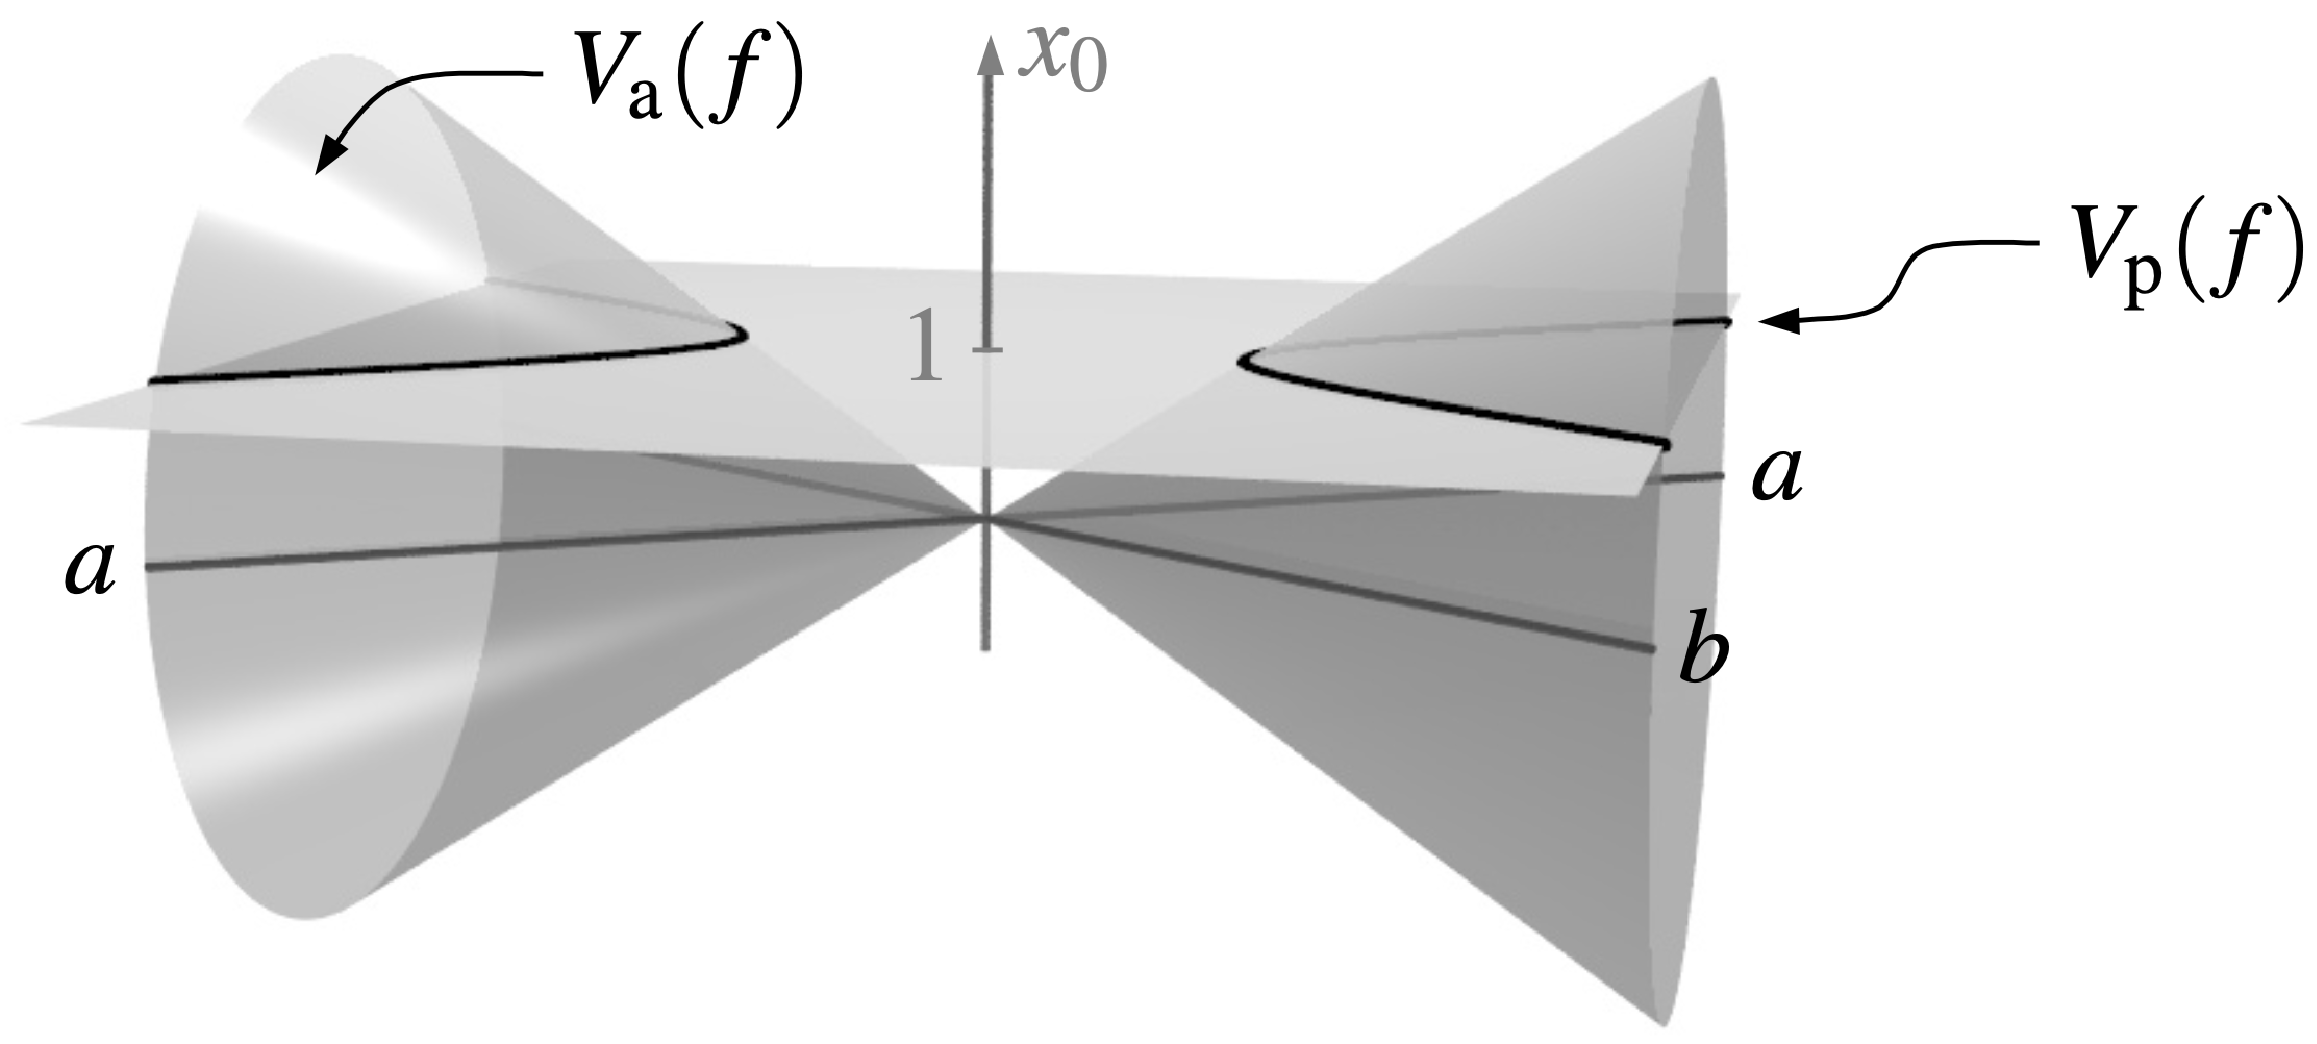
\includegraphics[width=.6\textwidth]{cone.pdf}
					\end{center}
					% \begin{tikzpicture}[thick]
					% 	\draw[->] (-3,0)--(3,0); \node[below] at (3,0) {$x_2$};
					% 	\draw[->] (0,-1)--(0,2.5); \node[right] at (0,2.5) {$x_0$};
					% 	\draw[<-] (-1.5,-.6)--(1.5,.6); \node[below] at (-1.5,-.8) {$x_1$};
					% 	\fill[gray!20,opacity=.7] (-4.5,.2)--(-1.5,1.4)--(4.5,1.4)--(1.5,.2)--cycle;
					% 	\draw (0,1.4)--(0,.8);
					% 	\fill[gray,opacity=.2] (-3,0) ellipse (0.6cm and 1.6cm);
					% 	\fill[gray,opacity=.2] (3,0) ellipse (.6cm and 1.6cm);
					% 	\fill[gray,opacity=.5] (-3,-1.6)--(0,0)--(-3,1.6) arc (90:270:.6cm and 1.6cm);
					% \end{tikzpicture}
				\end{eg}

				\begin{remark}
					Recall $\P^n$algebraic variety of dimension $n$, then hypersurface $X\subset\P^n$ is defined by $V_p(J)$ of dimension $n-1$. Hypersurfaces in $\AA^n$ have principal ideals, $X=V_a(f)$, $f\in\K$ (cf. Hauptidealsatz). Take $X\subset\P^n$ such that $Y=X\cap U_0$ ($U_0=\AA^n$ where $x_0=1$) is of dimension $n-1$. Then $I_a(Y)=(f)$ $\Longrightarrow$ $V_p(f^h)=X$ ($X=\bar{Y}$). Note: $I_a(Y)$ radical $\Longrightarrow$ $f$ has no repeated factors (e.g. $f\neq(x+1)^2$) $\Longrightarrow$ $f^n$ has no repeated factors $\Longrightarrow$ $(f^h)$ radical. Nullstellensatz: $I_p(X)=I_p(V_p(f^h))=(f^h)$, i.e. $I_p(X)$ principal. 
				\end{remark}

				\begin{remark}
					If $X,Y\subset\P^n$, then 
					\begin{enumerate}
						\item $I_p(X\cup Y)=I_p(X)\cap I_p(Y)$
						\item $I_p(X\cap Y)=\sqrt{I_p(X)+I_p(Y)}$, unless RHS=$I_0$
						\item $J=(f)$ $\Longrightarrow$ $J^h=(f^h)$
					\end{enumerate}
					Note that (iii) is not true if $J$ is not principal, i.e. $(f_1,\dots,f_n)^h\neq(f_1^h,\dots,f_n^h)$.
				\end{remark}

				\begin{exc}
					Find a counterexample for (iii).
				\end{exc}

				\begin{exc}
					Let $R\neq0$ be a graded ring. Show that $R$ integral domain if and only if for $f,g$ homogeneous, $fg=0$ $\Longrightarrow$ $f=0$ or $g=0$. 
				\end{exc}

				\begin{exc}
					Let $X$ be a projective algebraic set. Show $X$ irreducible $\Longleftarrow$ $S(X)$ integral domain.
				\end{exc}
			
			}			
		

		\subsection{Regular Functions}

			\noindent Goal: In analogy to affine varieties we would like to define a natural ringed space structure on projective algebraic sets, turning them into prevarieties. We can then show that they are actually varieties and study their properties.
			\\

			\noindent Difficulty: A homogeneous polynomial or a quotient of homogeneous polynomials does not provide a well-defined function on subsets of $\P^n$ (e.g. $f$ homogeneous of degree $d$: $f(\lambda x)=\lambda^df(x)$, but $[\lambda x]=[x]$ \contradiction).
			\\

			\noindent Notation: For a projective algebraic set $X\subset\P^n$ we write $S(X)=K[T_0,\dots,T_n]/I_p(X)$ for the coordinate ring of $X$ and $S(X)_d$ for its homogeneous component of degree $d$.

			\begin{defi}(Regular functions)
				Let $U$ be an open subset of a projective algebraic set $X$. A regular function on $U$ is a map $\phi:U\rightarrow K$ such that for any $a\in U$ there is an open neighbourhood $U_a\subset U$ of $a$ and homogeneous polynomials $f,g\in S(X)_d$ with $f(x)\neq0$ and $\phi(x)=\frac{g(x)}{f(x)}$ for all $x\in U_a$. We denote the set of regular functions on $U$ by $\O_X(U)$.
			\end{defi}

			\begin{prop}
				The functor $\O_X$ is a sheaf of $K$-algebras on $U$. We call this the structure sheaf of $X$.
			\end{prop}

			\begin{remark}
				One can show that the structure sheaf $X\subset\P^n$ coincides with its structure sheaf as a closed subprevariety of $\P^n$ (cf. \autoref{def--subprevarieties}).
			\end{remark}

			\begin{prop}\label{prop-projsets}(Projective algebraic sets are prevarieties)
				Let $X=V_p(J)\subset\P^n$ be a projective algebraic set. The sets 
				\begin{equation*}
					U_i=X\backslash V(x_i)=\{\x{n}\in X|x_i\neq0\}
				\end{equation*}
				form an affine open cover of $X$.
			\end{prop}
			\begin{proof}
				It is enough to show this for $i=0$. Consider the map
				\begin{equation*}
					\begin{tikzcd}[row sep=tiny,
						/tikz/column 2/.append style={nodes={anchor=base east}},
						/tikz/column 3/.append style={nodes={anchor=base west}}]
						F:V_a(J^i)\ar[r] & U_0,\, (x_1,\dots,x_n)\ar[r,mapsto] & {[1:x_1:\ldots:x_n]}\\
						& (\frac{x_1}{x_0},\dots,\frac{x_n}{x_0}) & \ar[l,mapsto]\x{n}
					\end{tikzcd}.
				\end{equation*}
				We claim that this is an isomorphism. By construction, $F$ and $F^{-1}$ are well-defined and inverse to each other. Thus, it suffices to show continuity and pullback to regular functions. For continuity, consider a closed subset $V_p(\tilde{J})\cap U_0=Z\subset U_0$ ($\tilde{J}\in K[x_0,\dots,x_n]$ homogeneous). Then $F^{-1}(Z)=V_a(\tilde{J}^i)$ is closed. On the other hand, for $V_a(J^\prime)=W\subset V_a(J^i)$ closed ($J^\prime\in\K$), have $F(W)=V_p(J^{\prime h})\cap U_0$ closed. What is left to show is the pullback of regular functions to regular functions: a regular function on an open subset of $U_0$ is locally written as $\frac{g(x_0,\dots,x_n)}{f(x_0,\dots,x_n)}$ with $f,g\in S(X)_d$ and $f\neq0$. Then 
				\begin{equation*}
					F^\ast\left( \frac{g(x_0,\dots,x_n)}{f(x_0,\dots,x_n)} \right)=\frac{g^i(x_1,\dots,x_n)}{f(x_1,\dots,x_n)}
				\end{equation*}
				is a regular function on $V_a(J^i)$ (as q quotient of polynomials with $f^i\neq0$). Conversely, for some regular function $\frac{g(x_1,\dots,x_n)}{f(x_1,\dots,x_n)}$ (locally) on an open subset of $V_a(J^i)$ with $f\neq0$, we have
				\begin{equation*}
					(F^{-1})^\ast\left(\frac{g(x_1,\dots,x_n)}{f(x_1,\dots,x_n)}\right)=\frac{g(\frac{x_1}{x_0},\dots,\frac{x_n}{x_0})}{f(\frac{x_1}{x_0},\dots,\frac{x_n}{x_0})}.
				\end{equation*}
				Upon multiplying both, numerator and denominator by $x_0^{\max\{\deg f,\deg g\}}$ this is a regular function on $U_0$. Hence, $U_0$ is an affine open subset of $X$. In particular, $\{U_i\}_{i=0,\dots,n}$ is an affine open cover of $X$.
			\end{proof}

			\begin{cor}
				The ringed space $(X,\O_X)$ is a prevariety.
			\end{cor}

		
		\subsection{Morphisms}
		
			\begin{prop}\label{prop--morphismproj}
				Let $X\subset\P^n$ be a projective algebraic set. If $f_0,\dots,f_m\in S(X)_d$ for some $d\in\N$, then
				\begin{equation*}
					f:X\backslash V(f_0,\dots,f_m)\rightarrow\P^m,x\mapsto[f_0(x):\ldots:f_m(x)]
				\end{equation*}
				is a morphism of prevarieties.
			\end{prop}
			\begin{proof}
				By virtue of the glueing property it is enough to look at an open cover $\{W_i\}_i$ of $X\backslash V(f_0,\dots,f_m)=:W$, where $W_i:=\{x\in W|f_i(x)\neq0\}$ such that $W_i=f^{-1}(U_i)$ with $U_i=\{y\in\P^m|y_i\neq0\}$ (usual open cover). Using affine corrdinates,
				\begin{equation*}
					f|_{W_i}(x)=\bigg(\frac{f_0(x)}{f_i(x)},\dots,\remove{\frac{f_i(x)}{f_i(x)}},\dots,\frac{f_m(x)}{f_i(x)}\bigg)
				\end{equation*}
				with $\frac{f_j}{f_i}$, $i\neq j$, regular functions on $W_i$. Then, by \autoref{prop--morphism}, $f|_{W_i}$ is a morphism on $W_i$ and by \autoref{rem--morphism} $f$ is.
			\end{proof}

			\noindent\underline{NB}: Cf. \autoref{prop--morphism} for affine varieties. Here, $f_i$ have to be homogeneous.

			\begin{eg}
				(Projection onto linear subspace) Consider the projection from $a=[1:0:\ldots:0]\in\P^n$ onto a linear subspace $V(x_0)$ of $\P^n$ (a linear subspace is a subspace $V(f_1,\dots,f_r)$ with $f_i$ homogeneous of degree one):
				\begin{equation*}
					f:\P^n\backslash\{a\}\rightarrow V(x_0)\simeq\P^{n-1},\x{n}\mapsto\x[1]{n}
				\end{equation*}
				where we forget about one of the homogeneous coordinates. Then $f$ is a morphsim by \autoref{prop--morphismproj}.
				\begin{center}
					\tikz[thick]{
						\draw (-2,0)--(2,0) node[right] {$V(x_0)\simeq\P^{n-1}$};
						\draw[dashed] (-1,-.5)--(.7,2.33);
						\fill (.5,2) circle [radius=.08cm] node[right] {$a$};
						\fill (0,1.167) circle [radius=.08cm] node[right] {$x$};
						\fill (-.7,0) circle [radius=.08cm] node[below right] {$f(x)$}
 						}
				\end{center}
				Pictorially, for some point $x=\x{n}$ the unique line through $x$ and $a$ is given by $\{[s:tx_1:\ldots:tx_n]|[s:t]\in\P^1\}$ and intersects $V(x_0)$ for $s=0,t=1$ (i.e. in $f(x)$ via $V(x_0)\simeq\P^{n-1}$).
			\end{eg}
		
		
		\subsection{Segre Embedding}

			\noindent We have seen in the last section that projective algebraic sets are prevarieties but, in fact, they are actually already varieties. In order to show that they are separated, we would like to have a convenient description of the product of two such varieties. This is provided by the Segre embedding.
			\\

			\noindent Construction: We embed $\P^m\times\P^n$ as a subprevariety of $\P^N$ with $N=(m+1)(n+1)-1$ (with coordinates $[z_{0,0}:\ldots:z_{m,n}]$) via
			\begin{equation*}
				f:\P^M\times\P^n\rightarrow\P^N,(\x{m},[y_0:\ldots:y_n])\mapsto[x_0y_0:\ldots:x_my_n]
			\end{equation*}
			(i.e. $z_{i,j}=x_iy_j$).

			\begin{prop}\label{prop--segre}
				The map $f$ as constructed above is an isomorphism onto $V_p(z_{i,j}z_{k,l}-z_{i,l}z_{k,j}|i,k=0,\dots,m,\,j,l=0,\dots,n)$.
			\end{prop}
			\noindent The map $f$ is called the Segre embedding and the coordinates $z_{i,j}$ the Segre coordinates on $\P^m\times\P^n$.
			\begin{proof}
				\begin{enumerate}
					\item Show $\im f=V_p(z_{i,j}z_{k,l}-z_{i,l}z_{k,j}|i,k=0,\dots,m,\,j,l=0,\dots,n)=:Y$:
					\begin{enumerate}
						\item [``$\subset$'':] Clear.
						\item [``$\supset$'':] Take $[z_{i,j}]_{i,j}\in Y$ and assume $0\neq z_{0,0}=1$. From the defining equations of $Y$ we find $z_{i,j}=z_{i,0}z_{0,j}$. Then define $x_i:=z_{i,0},y_j:=z_{0,j}$ $\Longrightarrow$ $[z_{i,j}]_{i,j}=f([x_i]_i,[y_j]_j)$.
					\end{enumerate}
					\item Show $f$ injective: Let $z\in Y$ such that $z_{0,0}=1$. If $f([x_i]_i,[y_j]_j)=[z_{i,j}]_{i,j}$ for some $([x_i]_i,[y_j]_j)\in\P^m\times\P^n$, then $x_0\neq0,y_0\neq0$. Hence, we can pass to affine coordinates and assume $x_0=1,y_0=1$. But then $x_i=z_{i,0},y_j=z_{0,j}$ for all $i=0,\dots,m$, $j=0,\dots,n$, i.e. $f$ injective.
				\end{enumerate}
				Similarly to (ii), one shows that $f,f^{-1}$ (locally in affine coordinates) are given by polynomial maps.
			\end{proof}

			\begin{cor}
				$\P^m\times\P^n\simeq Y$ is a prevariety.
			\end{cor}

			\begin{eg}
				Consider $\P^1\times\P^1\subset\P^3$. From \autoref{prop--segre} it follows that
				\begin{equation*}
					\P^1\times\P^1\overset{f}{\simeq} Y=\{[z_{0,0}:z_{0,1}:z_{1,0}:z_{1,1}]|z_{0,0}z_{1,1}=z_{1,0}z_{0,1}\}\subset\P^3.
				\end{equation*}
				In particular, \qt{lines} $\{a\}\times\P^1$, $\P^1\times\{a\}$ in $\P^1\times\P^1$ with $a$ constant are mapped to lines in $Y$:
				\begin{center}
					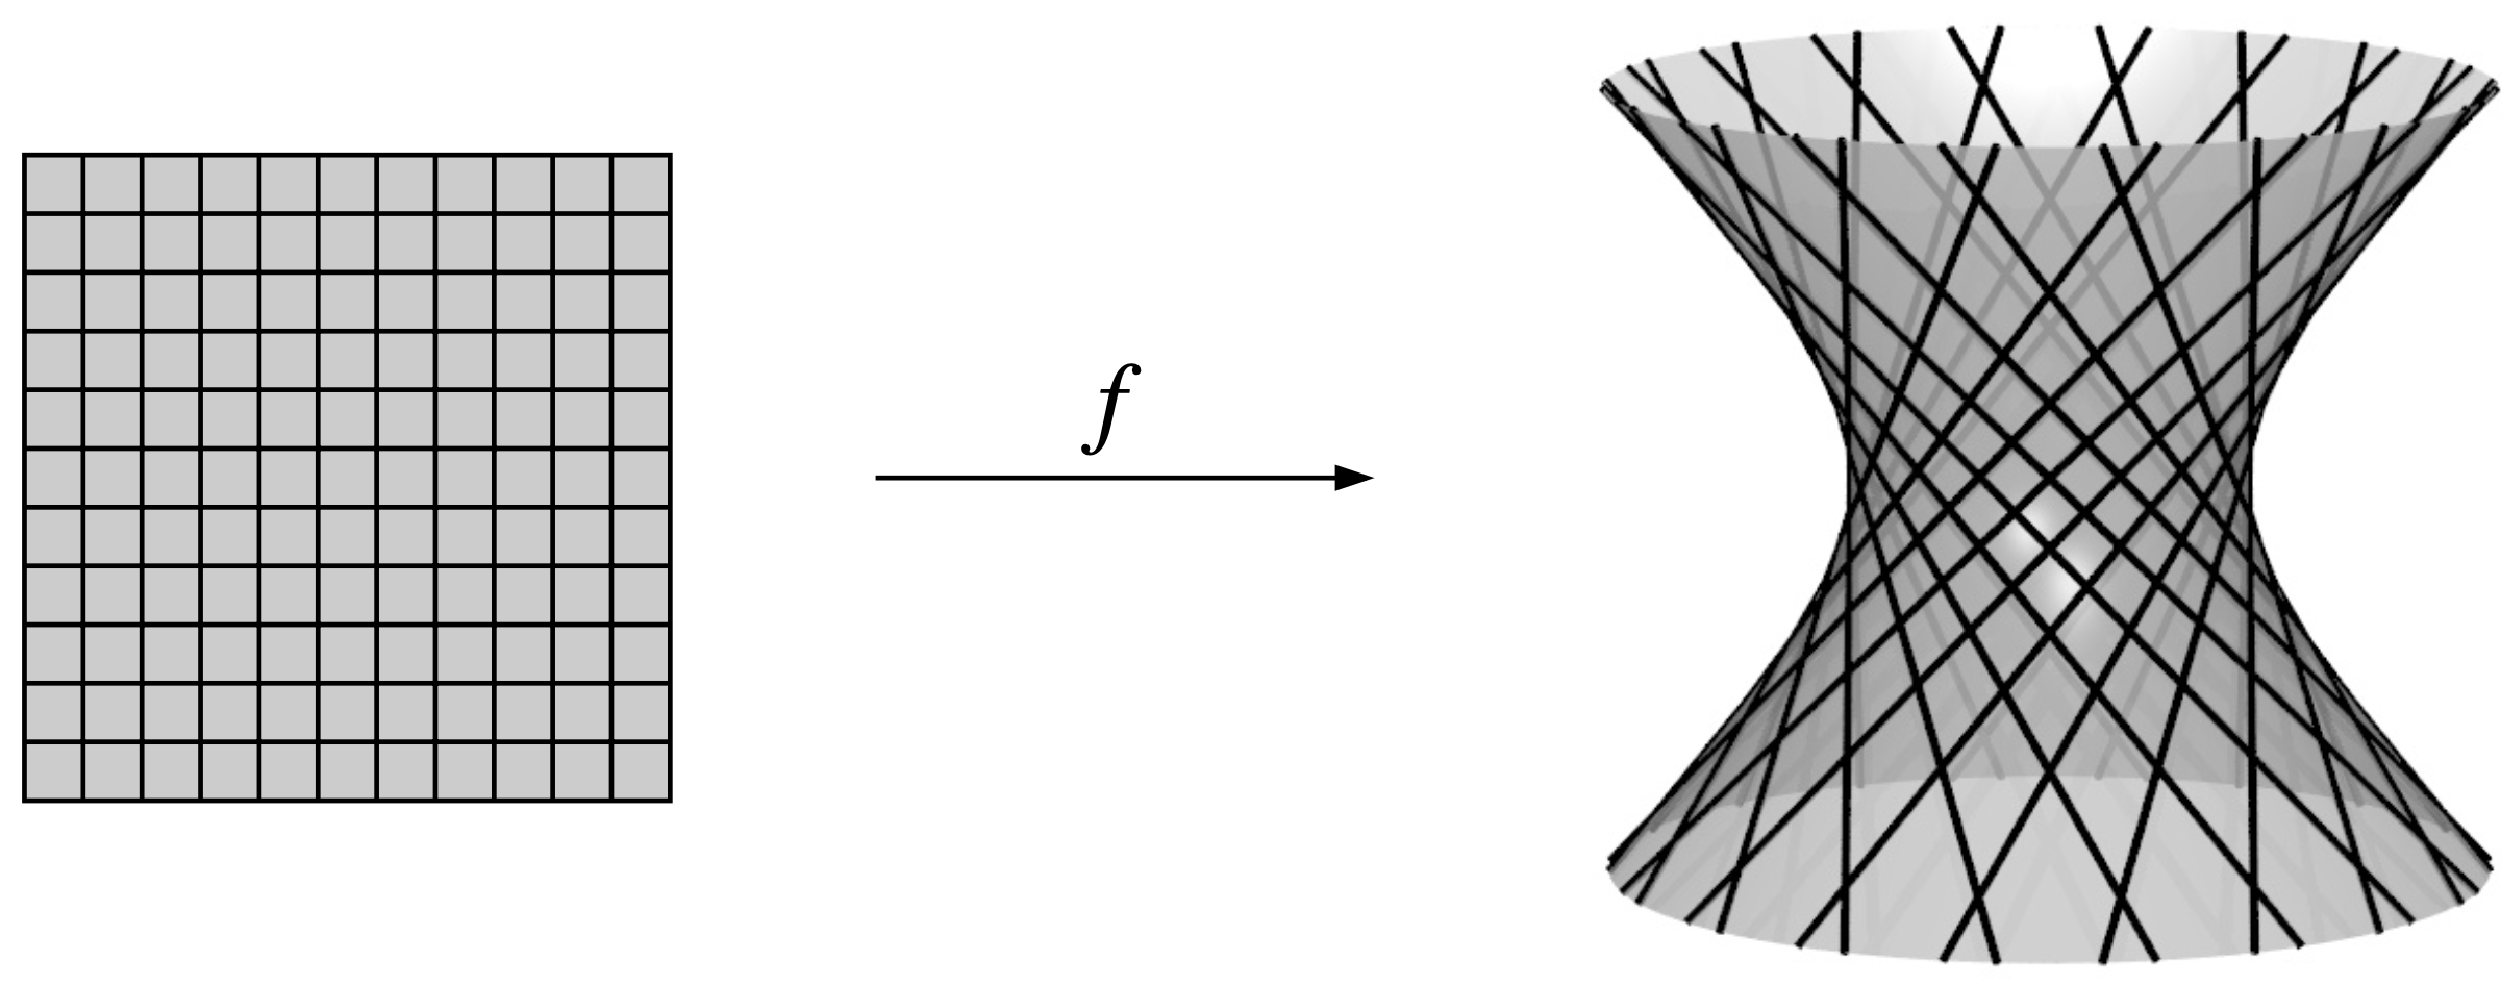
\includegraphics[width=.6\textwidth]{hyperbola.pdf}
				\end{center}
			\end{eg}

			\begin{cor}
				Projective prevarieties are separated, i.e. they are varieties.
			\end{cor}
			\begin{proof}
				We have to show that the diagonal is closed:
				\begin{align*}
					\Delta_{\P^n}=&\{(x,x)|x\in\P^n\}\\
					=&\{([x_0:\ldots:x_n],[y_0:\ldots:y_n])|\rank\begin{pmatrix}
						x_0 & \dots & x_n\\ y_0 & \dots & y_n
					\end{pmatrix}=1\}\\
					=&\{([x_0:\ldots:x_n],[y_0:\ldots:y_n])|\forall i,j=0,\dots,n:x_iy_j-y_ix_j=0\}.
				\end{align*}
				But the last line is just given by $V(z_{i,j}-z_{j,i})_{i,j}$ in Segre coordinates, which is closed in $Y=f(\P^n\times\P^n)$ $\Longrightarrow$ $\Delta_{\P^n}$ is closed in $\P^n\times\P^n$. Thus, $\P^n$ is a variety. But every subprevariety of a variety is already a variety by \autoref{ex--varieties}.
			\end{proof}

			{\color{gray}\subsection*{Comments on Projective Varieties}
			
				\begin{eg}
					Consider $S(\P^n)=K[T_0,\dots,T_n]$. For the structure sheaf $\O_X$ we find
					\begin{equation*}
						\O_X(U)=\{\phi:U\rightarrow K|\text{locally, }\phi=\frac{g}{f},\,f,g\text{ homogeneous of same degree, }f\neq0\}
					\end{equation*}
				\end{eg}

				\begin{prop}
					$\O_X(X)\not\simeq S(X)$.
				\end{prop}
				\begin{proof}
					By counterexample: take e.g. $\O_{\P^n}(\P^n)=K$.
				\end{proof}

				\begin{exc}
					Find $X,Y$ projective varieties with $X\simeq Y$ but $S(X)\not\simeq S(Y)$.
				\end{exc}

				\begin{exc}
					Show:
					\begin{enumerate}
						\item If $f:\P^n\rightarrow\P^m$ morphism with $n>m$, then $f$ is constant.
						\item $\P^n\times\P^m\not\simeq\P^{n+m}$ for any $n,m\ge1$ (hint: use universal property). 
					\end{enumerate}
				\end{exc}

				\begin{eg}
					An affine conic $X\subset\AA^2$ is an irreducible affine variety, $X=V_a(f)$ with $\deg f=2$. We claim $X\simeq V_a(x_2-x_1^2)$ or $X\simeq V_a(x_1x_2-1)$: Consider a projective conic $Y\subset\P^2$, irreducible, $Y=V_p(g)$ with $g$ homogeneous of degree 2. Set $X:=Y\cap\AA^2$.

					In fact, one can show that either isomorphism can be extended to a projective automorphism: with $p:=x_2-x_1^2$, $q:=x_1x_2-1$ have $Y\simeq V_p(p^h)$ or $Y\simeq V_p(q^h)$ with $p^h=x_0x_2-x_1^2$, $q^h=x_1x_2-x_0^2$. A coordinate change $x_1\leftrightarrow x_0$ shows $V_p(p^h)\simeq V_p(q^h)$.
				\end{eg}

				\begin{remark}
					There is an isomorphism
					\begin{equation*}
						\begin{tikzcd}[row sep=tiny,
							/tikz/column 1/.append style={nodes={anchor=base east}},
							/tikz/column 2/.append style={nodes={anchor=base west}},
							ampersand replacement=\&]
							f:V_p(p^h)\ar[r,"\simeq"] \& \P^1\\
							{[x_0^2:x_0x_1:x_1^2]} \& \ar[l,mapsto] [x_0:x_1]\\
							{[x_0:x_1:x_2]}\ar[r,mapsto] \& 
							\begin{cases}
								[x_1:x_2], & \text{if }[x_0:x_1:x_2]\neq[1:0:0]\\
								[x_0:x_1], & \text{if }	[x_0:x_1:x_2]\neq[0:0:1]
							\end{cases}
						\end{tikzcd}
					\end{equation*}
					This is well-defined by \autoref{prop--morphismproj}.
				\end{remark}
			
			}

		

		\subsection{Completeness}
			
			Goal: A useful analogue of compactness for the Zariski topology. If $K=\CC$, then in the classical topology, $\P^n$ is compact while $\AA^n$ is not.
			A Hausdorff space $X$ is compact if and only if the projection $X\times Y\rightarrow Y$, where $Y$ is any topologial space, is closed.

			\begin{defi}
				An algebraic variety $X$ is complete if the projection $\pi:X\times Y\rightarrow Y$ is closed for any algebraic variety $Y$.
			\end{defi}

			\begin{prop}\label{prop--proj-complete}
				The projective space $\P^n$ is complete.
			\end{prop}
			\begin{proof} We need to show the following:
				\begin{enumerate}
					\item The map $\pi:\P^n\times \P^m\rightarrow\P^m, (x,y)\mapsto y$ is closed: if $Z\subset\P^n\times\P^m$ is closed, then the condition $a\notin\pi(Z)$ is open. Use Segre embedding, $Z=V((f_1,\dots,f_r))$ where each $f_p$ is homogeneous of degree $d$ in $x_i,y_j$. Define $g_p=f_p(-,a)$ mapping from $\P^n$ ($a\in\P^m$). Now $a\notin\pi(Z)\Longleftrightarrow\nexists x\in\P^n:(x,a)\in Z\Longleftrightarrow V_p((g_1,\dots,g_r))=\emptyset\Longleftrightarrow (g_1,\dots,g_r)=(1)$ or $(g_1,\dots,g_r)=(x_1,\dots,x_r)\Longleftrightarrow\forall i\,\exists k_i: x_i^{k_i}\in(g_1,\dots,g_r)\Longleftrightarrow K[x_0,\dots,x_n]_k\subset(g_1,\dots,g_r)$ for some $k\ge d\Longleftrightarrow K[x_0,\dots,x_n]_k\overset{(\ast)}{=}(g_1,\dots,g_r)_k$. Now consider the map $F:(K[x_0,\dots,x_n]_{k-d})^{r}\rightarrow K[x_0,\dots,x_n]_k,(h_1,\dots,h_r)\mapsto \sum_{p=1}^{r}h_pg_p$. $(\ast)$ implies surjectivity of $F$. But a linear map is surjective if a minor is non-zero, i.e. some polynomial in the given coordinates in non-vanishing. This is precisely an open condition in the Zariski topology.
					\item $\P^n\times Y\rightarrow Y,(x,y)\mapsto y$ is closed whenever $Y$ is affine: if $Z\subset\P^n\times Y\rightarrow Y$ closed, embed $Y\subset\P^m$ and look at projective closure $\bar{Z}$ of $Z$ in $\P^n\times\P^m$. It satisfies $Z=\bar{Z}\cap(\P^n\times Y)$. Then, $\pi(Z)=\pi(\bar{Z}\cap(\P^n\times Y))=\pi(\bar{Z})\cap Y$. But $\pi(\bar{Z})$ closed in $\P^m$ by (i), hence $\pi(Z)$ closed in $Y$.
					\item $\P^n\times Y\rightarrow Y$ is closed for any variety $Y$: follows from (ii) by glueing.
				\end{enumerate}
			\end{proof}

			\begin{prop}
				\begin{enumerate}
					\item Any closed subvariety of a complete variety is complete.
					\item Any projective variety is complete.
					\item Affine space $\AA^n$ is not complete for any $n\ge1$.
					\item The image of a complete variety $X$ under a morphism $F:X\rightarrow Y$ of varieties is closed in $Y$.
					\item Any global regular function on a connected complete variety is constant: $\O_X(X)=K$.
				\end{enumerate}
			\end{prop}
			\begin{proof}
				\begin{enumerate}
					\item Let $X$ complete variety, $X^\prime\subset X$ closed subvariety. Take $Z\subset X^\prime\times Y$ closed  $\Longrightarrow Z\subset X\times Y$ closed $\Longrightarrow$ $\pi(Z)\subset Y$ closed.
					\item Follows from \autoref{prop--proj-complete}.
					\item It is enough to consider $\AA^1$. Let $\pi:\AA^1\times\AA^1\rightarrow\AA^1, (x,y)\mapsto y$ and $Z=V((T_1T_2-1))$. Then $\pi(Z)=\AA^1\backslash\{0\}$ is not closed. 
					\item The graph $\Gamma_f$ is closed since $Y$ is variety, and the image of $f$ is the projection of $\Gamma_f$ onto $Y$.
					\item Consider $\O_X(X)\ni\phi:X\rightarrow\AA^1\subset\P^1$, i.e. $\phi:X\rightarrow\P^1$ not surjective. The image is colsed by (iv), hence finite (in $\AA^1$). $X$ assumed connected, hence the image is a single element, i.e. $\phi$ constant.
				\end{enumerate}
			\end{proof}

		\subsection{Veronese Embedding}

			Idea: A \qt{degree $d$ embedding} of $\P^n$ into $\P^N$ ($N>n$), thus transferring degree $d$ equations to linear equations.
			\\Let $N+1=\binom{n+d}{n}$ be the number of monomials of degree $d$ in $x_0,\dots,x_n$. Call them $f_0,\dots,f_N$.

			\begin{prop}
				The map $F:x\mapsto[f_0(x),\dots,f_N(x)]$ defines an isomorphism from $\P^n$ onto the projective variety $F(\P^n)\subset\P^N$.
			\end{prop}
			\begin{proof}
				Observe $\{x_i^d\}_{i=0,\dots,n}\subset\{f_0,\dots,f_N\}$. These have no common zeros, i.e. we have $V_p(f_0,\dots,f_N)=\emptyset$. $F(\P^n)$ complete, hence closed in $\P^N$.\\ We can define an inverse of $F$: on patch $x_i=1$, for any $j$ can write $x_j=x_jx_i^d/x_i^d$ and map back to $x_j$. 
			\end{proof}

			For any ordering of the $f_i$, the map $F$ is called the degree $d$ Veronese embedding. The coordinates on $\P^N$ are called the Veronese coordinates on $\P^n$. This can be extended to any projective variety $X\subset\P^n$.

			\begin{prop}
				If $X\subset\P^n$ is a projective variety an $f\in S(X)_d$ with $d\ge1$, then $X\backslash V(f)$ is an affine variety.
 			\end{prop}
			\begin{proof}
				Have three possible cases: (i) $f=x_0$: $X\backslash V(f)=\AA^n$; (ii) $f$ linear: use projective automorphism $f=x_0$ and use (i); (iii) general case: degree $d$ Veronese embedding $F:\P^n\rightarrow\P^N$. Then $F(X)$ projective variety in $\P^N$, $f$ linear in Veronese coordinates and use (ii).
			\end{proof}


		\subsection{Rational Maps}

			Problem: Algebraic geometry is about understanding varieties via their regular functions. But there are no non-constant global regular functions on complete varieties.
			\\

			\noindent Remedy: Allow functions that are undefined on \qt{small} sets (cf. meromorphic functions). More generally, allow maps defined only on dense open subsets. This provides a way to deal with varieties having bad points (singularities).
			\\

			\noindent Let $X$ and $Y$ be algebraic varieties.
			\\

			\noindent Idea: Study functions defined on a dense open subset, up to equality on a dense subset.

			\begin{defi}
				(Rational maps) Consider pairs $(U,f)$ of a dense open subset $U\subset X$ and a morphism $f:U\rightarrow Y$. Two pairs $(U,f)$ and $(V,g)$ are equivalent, if $f|_W=g|_W$ for some dense open $W\subset U\cap V$. A rational map from $X$ to $Y$ is an equivalence class of a pair $(U,f)$. We write $f:X\dashrightarrow Y$. We say that $f$ is defined at $x\in X$ if $x\in U^\prime$ with $(U^\prime,f^\prime)$ in the equivalence class.
			\end{defi}

			\begin{eg}
				\begin{enumerate}
					\item Any morphism $f:X\rightarrow Y$ is a rational map.
					\item $\P^1\dashrightarrow \AA^1, [x_0:x_1]\mapsto\frac{x_1}{x_0}$ for all $[x_0:x_1]$ with $x_0\neq$. In particular, maximal dense open subset $\{[x_0:x_1]|x_0\neq1\}$.
					\item $\AA^2\dashrightarrow\AA^2, (x,y)\mapsto \frac{1}{x}$
				\end{enumerate}
			\end{eg}

			\begin{remark}
				If	$f,g:W\rightarrow Y$ are morphisms and $Y$ a variety, then $f=g$ if and only if they agree on a dense open subset $W^\prime\subset W$. In other words, the restriction $\O_W(W)\rightarrow \O_W(W^\prime)$ is injective. Consequences:
				\begin{enumerate}
					\item $(U,f)\sim(V,g)\Longleftrightarrow f|_{U\cap V}=g|_{U\cap V}$
					\item Each rational map $X\dashrightarrow Y$ has a representative $(U,f)$ with $U$ maximal. If $(V,g)\sim(U,f)$, then $V$ is dense in $U$ and $g=f|_{V}$.	
				\end{enumerate}
				This justifies dropping the open set in the notation of a rational map.
			\end{remark}

			\begin{defi}
				A rational function on an algebraic variety $X$ is a rational map $X\dashrightarrow \AA^1$. The set of rational functions is denoted by $K(X)$.
			\end{defi}

			Sums and products of rational functions are rational functions.

			\begin{prop}
				If $X$ is an irreducible algebraic variety, then $K(X)$ is a field.
			\end{prop}
			\begin{proof}
				Consider $(U,\phi)\in K(X)$. Then $(U\backslash V(\phi),\frac{1}{\phi})$ with $U\backslash V(\phi)$ open and dense since $X$ irreducible. Thus, can make everything invertible by disregarding small number of points (i.e. closed sets).
			\end{proof}

			\begin{remark}
				Let $X$ be an irreducible algebraic variety.
				\begin{enumerate}
					\item If $\emptyset\neq U\subset X$ is open, then $K(U)\simeq K(X)$.
					\item $K(X)$ is the fraction field of $\O_X(U)$ for any affine open subset $U\neq\emptyset$.\\$[[\text{Enough to check: $K(U)\simeq\Frac(\O_U(U))$ when $U$ is affine.}]]$
				\end{enumerate}
			\end{remark}

			\begin{defi}
				A rational map $f:X\dashrightarrow Y$ of algebraic varieties is dominant if its image contains a dense open subset of $Y$.
			\end{defi}

			If $X$ and $Y$ are irreducible, then $f$ induces $f^\ast:K(Y)\rightarrow K(X)$: 
			\begin{equation*}
				\begin{tikzcd}
					X\ar[r,dashed,"f"]\ar[rr,dashed,"f^\ast\phi"',bend right] & Y\ar[r,dashed,"\phi"] & \AA^1
				\end{tikzcd}
			\end{equation*}

			\begin{thm}
				\phantom{x}\\The assignment $X\rightarrow K(X), f\mapsto f^\ast$ defines a contravariant equivalence from the category of irreducible algebraic varieties with dominant rational maps as morphisms to the category of finitely generated field extensions of $K$.
			\end{thm}

		\subsection{Birationality}
			
			Idea: Invertibility on a dense open subset. 
			\\

			\noindent Note: If $f:X\dashrightarrow Y$ is dominant and $g:Y\dashrightarrow X$ is  a rational map, then $g\circ f$ is a rational map $X\dashrightarrow X$.

			\begin{defi}
				A map $f:X\dashrightarrow Y$ of algebraic varieties is birational if it is dominant and there is a dominant rational map $g:Y\dashrightarrow X$ with $g\circ f=\id_X$ and $f\circ g=\id_Y$ as rational maps. Then $X$ and $Y$ are said to be birationally equivalent.
			\end{defi}

			\begin{prop}
				The following statements are equivalent for irreducible varieties $X$, $Y$:
				\begin{enumerate}
					\item $X$ and $Y$ are birationally equivalent.
					\item There exist non-empty open subsets $U\subset X$ and $V\subset Y$ with $U\simeq V$.
					\item $K(X)\simeq K(Y)$
				\end{enumerate}
			\end{prop}
			\begin{proof}\phantom{x}
				\begin{enumerate}[leftmargin=5em]
					\item[(ii)$\Rightarrow$(i):] $f:U\rightarrow V\subset Y$, $f^{-1}:V\rightarrow U\subset X$. By definition, $f:X\dashrightarrow Y$ birational since it is dominant ($\im f=V$) and $f^{-1}$ is dominant as well.
					\item[(i)$\Rightarrow$(ii):] Have $g:X\dashrightarrow Y$ defined on $W_g$, $h:Y\dashrightarrow X$, defined on $W_h$. Then take $U=W_g\cap g^{-1}(W_h)$, $V=W_h\cap h^{-1}(W_g)$. Restriction to these sets gives isomorphism from $U$ to $V$. 
					\item[(ii)$\Rightarrow$(iii):] $K(X)\overset{U\text{ dense}}{\simeq} K(U)\overset{\text{Functoriality}}{\simeq} K(V)\overset{V\text{ dense}}{\simeq} K(Y)$
					\item[(iii)$\Rightarrow$(ii):] $K(X)\rightarrow K(Y)$  induced by $f:X\dashrightarrow Y$ with \qt{inverse} $g:Y\dashrightarrow X$, i.e. $f:U_0\rightarrow Y$, $g:V_0\rightarrow X$. Take $U=f^{-1}(V_0)\subset X$ and $V=g^{-1}(U_0)\subset Y$.
				\end{enumerate}
			\end{proof}

			\begin{defi}
				An algebraic variety is rational if it is birationally equivalent to an affine space $\AA^n$.
			\end{defi}

			\begin{eg}
				Projective space is rational. Every quadratic hypersurface in $\P^n$ is birationally equivalent to $\P^{n-1}$, hence rational.
			\end{eg}

		{\color{gray}\subsection*{Comments on Completeness and Rational Maps}

			\begin{prop}
				$f:X\rightarrow Y$ morphism of varieties, $X$ complete $\Longrightarrow$ $f(X)$ closed in $Y$.
			\end{prop}

			\begin{exc}
				Given $f:X\rightarrow Y$, consider $X\rightarrow X\times Y\overset{\pi}{\rightarrow} Y$, $x\mapsto(x,f(x))\mapsto f(x)$. Can we use this to claim that if $f:X\rightarrow Y$ is closed for all $Y$, then $X$ complete? 
			\end{exc}

			\begin{exc}
				$f:X\rightarrow Y$, $X$ complete. Is $f(X)$ complete?\\
				Solution: Yes! Consider the commutative diagram with $W$ variety,
				\begin{equation*}
					\begin{tikzcd}
						X\times W\ar[dr,"\pi"]\ar[rr,"f\times \id"] & & f(X)\times W\ar[dl,"\pi"']\\
						& W &
					\end{tikzcd}
				\end{equation*} 
				Let $Z\subset f(X)\times W$ closed. Define $Z^\prime:=(f\times\id)^{-1}(Z)$. Then $\pi(Z^\prime)=\pi(Z)$, so $\pi(Z)$ is closed since $X$ is complete.
			\end{exc}

			\begin{exc}
				Show if $X$ is such that $\pi:X\times Y\rightarrow Y, (x,y)\mapsto y$ is closed for all affine $Y$, then $X$ is complete.
			\end{exc}

			\subsubsection*{Completeness:}
			
			Let $f(x)$ closed in any $Y$. $Y$ irreduible, $\dim Y=\dim X\Longrightarrow f(X)=Y$. This is contrary to $\AA^n\hookrightarrow\P^n$ (missing many points, namely the ones at infinity).

			\begin{remark}
				Any projective variety is complete. But there exist complete non-projective varieties (Hironaka's example), which are pathological.
			\end{remark}

			\begin{eg}
				Grassmannians are projective varieties,
				\begin{equation*}
					G(k,n)=\{\text{all $k$-dimensional linear subspaces of $K^n$}\}	
				\end{equation*}
				(cf. flag varieties/manifolds). Consider the map
				\begin{equation*}
					G(k,n)\rightarrow K^{\binom{n}{k}}\rightarrow \P^{\binom{n}{k}-1},\, x=\spa(v_1,\dots,v_k)\mapsto v_1\wedge\dots\wedge v_k\mapsto p(x).
				\end{equation*}
				Can show: well-defined, coordinate functions are polynomials, injective, image is closed: some determinants are zero. This is the Plücker embedding (cf. [G1] chapter 8).
			\end{eg}

			\subsubsection*{Rational maps and functions:}

			$f:X\dashrightarrow Y$, $X,Y$ algebraic varieties means $f$ is defined on a dense open subset $U\subset X$. $f:U\rightarrow Y$ morphism.\\

			\noindent A rational function is a rational map $f:X\dashrightarrow\AA^1$. If $X$ irreducible, then $\{f:X\dashrightarrow\AA^1\}=K(X)$ is a field. Special case: $X$ affine $\Longrightarrow$ $K(X)=\Frac(\O_X(X))$.

			\begin{remark}
				$X$ affine, irreducible: $K(X)=\O_X(X)_{I(X)}=\O_X(X)_{(0)}=\Frac(\O_X(X))$.
			\end{remark}

			\noindent\underline{NB}: $X$ irreducible $\Longrightarrow$ $I(X)$ prime and hence $\O_X(X)$ integral domain.

			\begin{remark}
				$X$ affine, not necessarily irreducible, then 
				\begin{equation*}
					\{\text{rational functions $f:X\dashrightarrow\AA^1$}\}=S^{-1}\O_X(X)
				\end{equation*}
				with 
				\begin{align*}
					S=&\{f\in\O_X(X)|\forall X_0\subset X\text{ irred. comp.}:f|_{X_0}\notin I(X_0)\}\\
					=&\{\text{non-zero divisors $\neq0$ in $\O_X(X)$}\}
				\end{align*}
			\end{remark}

			\begin{remark}
				$f:X\dashrightarrow\AA^1$ rational map defined on $D_f$ open, $f:D_f\rightarrow\AA^1\rightarrow\P^1, x\mapsto [1:f(x)]$. Can extend $f$ to $D_f\cup D_{1/f}$ ($D_{1/f}$ set where $f\neq0$), $D_{1/f}\rightarrow\P^1,x\mapsto[\frac{1}{f(x)}:1]$. Points in $X\backslash(D_f\cup D_{1/f})$ are called points of indeterminacy.
			\end{remark}

			\begin{eg}
				$f:\AA^2\dashrightarrow\AA^1,(x_1,x_2)\mapsto\frac{x_1}{x_2}$ and $1/f:(x_1,x_2)\mapsto\frac{x_2}{x_1}$. Point of indeterminacy: $(0,0)$.
			\end{eg}}





	\section{Smooth Varieties}\label{sec--smooth-varieties}

		\subsection{Tangent Spaces}

			\subsubsection*{Tangent Space Concretely}

				Intuition: A curve is smooth at a point if it has a well-defined tangent line (linearization) there. A variety is smooth at a point if it has a tangent space of the same dimension there. 
				\\

				The tangent space of $X$ at $a$ is the zero set of linear equations whose coefficients are the values of $\frac{\partial f}{\partial T_i}$ at $a$, for $f\in I(X)$.
				\\

				The formal derivative $\pd{f}{T_i}$ of $f\in\K$ is defined by extending $\pd{T^d_i}{T_i}=dT^{d-1}_i$ linearly over $K[T_1,
				\dots,\remove{T_i},\dots,T_n]$.

				\begin{defi}\label{def--tangentspace}
					The tangent space $T_aX$ of an affine variety $X\subset\AA^n_K$ at $a=(a_1,\dots,a_n)\in X$ is the set of all $(x_1,\dots,x_n)\in\AA^n$ with 
					\begin{equation*}
						\forall f\in I(X):\,\sum_{i=1}^n\pd{f}{T_i}(a)(x_i-a_i)=0.
					\end{equation*}
				\end{defi}

				\begin{remark}
					\begin{enumerate}
						\item $T_aX$ is a vector subspace of $\AA^n$ with origin $a$.
						\item Translating $X$, we may always assume $a=(0,\dots,0)$. Then $T_aX=V(f_1|f\in I(X))=V(f_1|f\in S)$ for any set $S$ generating $I(X)$ (where $f_1$ denotes degree one-part of $f$).\\
						$[[f,g\in I(X): f_1(x)=0,g_1(x)=0\Longrightarrow (f+g)_1(x)=0\text{ and also }h\in I(X): (hf)_1(x)=h(0)f_1(x)+f(0)h_1(x)=0]]$.\\
						\item Remark (ii) implies, in particular, that the system of linear equations is finite.
					\end{enumerate}
				\end{remark}

				\begin{eg}
					\begin{enumerate}
						\item $X=V(T_2-T_1^2)$, then $T_aX=V(T_2)$
						\item $X=V(T_2^2-T_1^2-T_1^3)$, then $T_aX=V(0)=\AA^2$
						\item $X=V(T_2^2-T_1^3)$, then $T_aX=V(0)=\AA^2$
					\end{enumerate}
					\vspace{1em}
					\tikz{\node at (0,-1.5){(i)};\draw[gray] (0,-1)--(0,1);\draw[gray](-1,0)--(1,0);\node [above] at (0,1) {$x_2$};\node[right] at (1,0) {$x_1$};\draw[thick]plot[smooth] file {plots/parabola.table}}\hfill\tikz{\node at (0,-1.5){(ii)};\draw[gray] (0,-1)--(0,1);\draw[gray](-1,0)--(1,0);\node [above] at (0,1) {$x_2$};\node[right] at (1,0) {$x_1$};\draw[thick,black]plot[smooth] file {plots/cubic1.table};\draw[thick,black]plot[smooth] file {plots/cubic2.table}}\hfill\tikz{\node at (0,-1.5){(iii)};\draw[gray] (0,-1)--(0,1);\draw[gray](-1,0)--(1,0);\node [above] at (0,1) {$x_2$};\node[right] at (1,0) {$x_1$};\draw[thick,black]plot[smooth] file {plots/neil1.table};\draw[thick,black]plot[smooth] file {plots/neil2.table}}
				\end{eg}

			\subsubsection*{Tangent Space Abstractly}

				In practice, define $T_aX$ by taking an affine open $U\subset X$ containing $a$, embedding $U$ in $\AA^n$ and setting $T_aX:=T_aU$.
				\\

				Is this independent of all choices involved? Yes:
				\\

				\begin{prop}(Tangent Space)\label{prop--tangentspace}
					Let $R=\O_{X,a}$ be the local ring at $a$ with unique maximal ideal $m=I_a$. Then $m/m^2$ is a vector space over $K$ and its dual is isomorphic to $T_aU$.
				\end{prop}

				In order to prove this, we need the following results:

				\begin{thm}\phantom{k}\\
					The map $f\mapsto f_1$ induces a natural vector space isomorphism $I(\{a\})/I(\{a\})^2\simeq(T_aX)^\ast$, where $I(\{a\})\subset\O_X(X)$ is the ideal of $a$.
				\end{thm}
				\begin{proof}
					Consider 
					\begin{equation*}
						\K/I(X)=\O_X(X)\supset I(\{a\})\overset{\phi}{\longrightarrow} (T_aX)^\ast=\Hom_K(T_aX,K), \bar{f}\mapsto f_1|_{T_aX}.
					\end{equation*}
					This is well-defined: if $\bar{f}=\bar{g}\Longrightarrow f-g\in I(X)\Longrightarrow (f-g)_1|_{T_aX}=0\Longrightarrow f_1|_{T_aX}=g_1|_{T_aX}$. Moreover, it is linear and surjective: any linear form in $(T_aX)^\ast$ can be extended to a linear form in the ambient space $\Hom(K^n,K)$ which is given in the above way. We need to show that $\ker\phi=I(\{a\})^2$.
					\begin{enumerate}
						\item[``$\subset$'':] Assume $\bar{f}\in\ker\phi$ such that $f_1|_{T_aX}=0$. Further assume that there is $g\in I(X): g_1=f_1$. Then $\bar{f}=\overline{f-g}\in I(\{a\})^2$ as $f-g$ has no constant and linear term. Such a $g$ can always be found for $f$ for the following reason: set $\dim T_aX=:d$. Consider the vector subspaces $\{g_1|g\in I(X)\}$, $\{h:K^n\rightarrow K|\,h|_{T_aX}=0\}$. Both have dimension $n-d$ and all $g_1$ in the first set vanish at the tangent space, hence we have $\subset$. But two such vector subspaces of same dimension must be equal. Thus, any linear form that vanishes on $T_aX$ actually is the linear part of a function in $I(X)$. 
						\item[``$\supset$'':] Consider $\bar{f},\bar{g}\in I(a)\Longrightarrow (fg)_1=f(0)g_1+g(0)f_1=0\cdot g_1+0\cdot f_1=0$.
					\end{enumerate}
				\end{proof}

				Let $X$ be an affine variety, $s\in X$ and $I_a$ the unique maximal ideal of $\O_{X,a}$. Recall that $I_a$ is the localisation of $I(\{a\})$.

				\begin{prop}
					Localisation induces an isomorphism $I(\{a\})/I(\{a\})^2\simeq I_a/I_a^2$.
				\end{prop}
				\begin{proof}
					Note that $\O_{X,a}=\O_X(X)_{I(\{a\})}=S^{-1}\O_X(X)$ with $S=\O_X(X)\backslash I(\{a\})$. To perform all steps properly we need to know about the localisation of modules which we do not want to introduce at this point. We can still understand the idea. First, $S^{-1}I(\{a\})=I_a$, $S^{-1}I(\{a\})^2=I_a^2$ and $S^{-1}(I(\{a\})/I(\{a\})^2)=I_a/I_a^2$. Take $\frac{g}{f}\in S^{-1}I(\{a\})$ with $g(a)=0,f(a)\neq 0$. Then $\frac{g}{f}=\frac{g}{\lambda}\modd I(\{a\})^2$ (where $\lambda\in K$). Then $f=f(a)+h$ with $h\in I(\{a\})\Longrightarrow gf=gf(a)+gh$ with $gh\in I(\{a\})^2$, so $gf=gf(a)$ in $I(\{a\})/I(\{a\})^2$.
				\end{proof}

				This finally proves \autoref{prop--tangentspace}. Now we are in a position to define the tangent space for general algebraic varieties in a way that agrees with the concrete \autoref{def--tangentspace} upon choosing an affine chart containing $a$.

				\begin{defi}
					Let $X$ be an algebraic variety and $a\in X$. The tangent space $T_aX$ of $X$ at $a$ is the $K$-vector space dual to $I_a/I_a^2$, where $I_a$ is the unique maximal ideal of $\O_{X,a}$
				\end{defi}

				\noindent\underline{NB}: $(I_a/I_a^2)^\ast=T_aX\Longleftrightarrow I_a/I_a^2\simeq(T_aX)^\ast$

				\begin{remark}
					\begin{enumerate}
						\item The local ring $\O_{X,a}$ is, by construction, independent of both the choice and embedding of an affine cover.
						\item The tangent space can be obtained concretely using the linear equations associated to any affine open $U\ni a$.
					\end{enumerate}
				\end{remark}

				Therefore, it is enough to consider the affine case.

		\subsection{Smoothness}

			\begin{prop}\label{prop--smoothness}
				Let $X$ be an algebraic variety.
				\begin{enumerate}
					\item $\dim T_aX\ge\codim_X\{a\}$
					\item For each $n\in\N$, the set of all $a\in X$ with $\dim T_aX\ge n$ is closed.
				\end{enumerate}
			\end{prop}
			\begin{proof}
				(Sketch)
				\begin{enumerate}
					\item May assume $X$ affine, irreducible. $I_a/I_a^2$ has basis $\{f_1+I_a^2,\dots,f_d+I_a^2\}$. Nakajama lemma implies $I_a$ has basis $\{f_1,\dots,f_d\}$. Then $I(a)=(f_1,\dots,f_d)$, $0=\dim V(I(a))\ge\dim X-d$ $\Longrightarrow$ $d\ge\dim X$.
					\item Again, reduce to affine setting and see that from concrete definition of tangent space, this amounts to some minors vanishing, so the rank of $\left(\pd{f_i}{T_j}\right)$ being at most something. This condition is closed.
				\end{enumerate}
			\end{proof}

			\begin{defi}
				A point $a\in X$ is called smooth (also regular, non-singular) if $\dim T_aX=\codim_X\{a\}$ and singular otherwise. If $X$ only contains smooth points it is called smooth, otherwise it is called singular. 
			\end{defi}

			\begin{cor}
				The set of smooth points is open in $X$.
			\end{cor}
			\begin{proof}
				The set of all points with $\dim T_aX\ge\codim_X\{a\}+1$ is closed, hence set of smooth points in $X$ is open.
			\end{proof}

			In fact, one can show that in any irreducible component of $X$ there exist smooth points. Hence, in any irreducible component the set of smooth points is non-empty and because it is open, it is dense. I.e. any algebraic variety has a dense open subset of smooth points (\qt{most points} are smooth).

			\begin{eg}
				Consider $X=V(T_2-T_1^2)$. Then $\dim T_0X=1$, whereas for  $X=V(T_2^2-T_1^3), X=V(T_2^2-T_1^3-T_1^2)$ we find $\dim T_aX=2>1=\codim_X\{a\}$.
			\end{eg}

			\begin{thm}(Jacobi criterion)\\
				Let $X\subset\AA^n$ be an affine variety with $I(X)=(f_1\dots,f_m)$. A point $a\in X$ is smooth if and only if the $m\times n$ Jacobian matrix 
				\begin{equation*}
					J=\left(\pd{f_i}{T_j}(a)\right)_{ij}
				\end{equation*}
				satisfies $\rank J\ge n-\codim_X\{a\}$. Then $\rank J=n-\codim_X\{a\}$.
			\end{thm}
			\begin{proof}
				We have $T_aX=\ker J$. $a$ is smooth if and only if $\dim\ker J\le \codim_X\{a\}$. From linear algebra, $\dim\ker J=n-\rank J$.
			\end{proof}

			{\color{gray}\subsubsection*{Comments on Tangent Space and Smoothness:}

				Denote $A=\O_{X,a}$, $m=I_a$ maximal ideal.
				\\

				\noindent There are different guises of $T_aX$:
				\begin{equation*}
					\begin{tikzcd}[row sep=.1cm,
						/tikz/column 1/.append style={nodes={anchor=base east}},
						/tikz/column 2/.append style={nodes={text width=width("$Derk(AlK)$"), text centered}},
						/tikz/column 3/.append style={nodes={anchor=base west}}]
						\Hom_{K-\text{alg}}(A,K[\epsilon])\ar[r,"\simeq"] & \der_K(A,K)\ar[r,"\simeq"] & \Hom_K(m/m^2,K)\\
						(\phi:a\mapsto\phi_0(a)+\phi_1(a)\epsilon)\ar[r,mapsto] & \phi_1 &\\
						& D\ar[r,mapsto] & D|_m
					\end{tikzcd}
				\end{equation*}
				and from scheme theory we have
				\begin{equation*}
					\begin{tikzcd}
						\{a^\prime\in X(K[\epsilon])|a^\prime\rightarrow a\text{ for }\epsilon\mapsto 0\}\ar[r,"\simeq"] & \Hom_{K-\text{alg}}(A,K[\epsilon])
					\end{tikzcd}
				\end{equation*}
				
				\begin{defi}
					A derivation from a $K$-algebra $A$ to an $A$-module $M$ is a map $\mathrm{d}:A\rightarrow M$ satisfying
					\begin{enumerate}
						\item $\mathrm{d}(\lambda\cdot 1)=0$ for all $\lambda\in K$
						\item $\mathrm{d}(f+g)=\mathrm{d}f+\mathrm{d}g$
						\item $\mathrm{d}(fg)=g\mathrm{d}f+f\mathrm{d}g$
					\end{enumerate}
					We denote the set of derivations $A\rightarrow M$ by $\der(A,M)$.
				\end{defi}

				\noindent\underline{NB}: $K\simeq A/m$, so $K$ is an $A$-module.
				\\

				\noindent\underline{NB}: Morally, $T_aX$ consists of derivations (\qt{directed derivatives}).
				\\

				\noindent\underline{NB}: The isomorphism $\der_K(A,K)\simeq\Hom_K(m/m^2,K)$ is a universal property: for all derivations $\mathrm{d}:A\rightarrow K$ there is a unique $\phi:m/m^2\rightarrow K$ such that 
				\begin{equation*}
					\begin{tikzcd}
						A\ar[r,"\Delta"]\ar[dr,"\mathrm{d}"'] & m/m^2\ar[d,dashed,"\exists !\,\phi"]\\
						& K
					\end{tikzcd}
				\end{equation*}
				commutes, with $\Delta(f)=f-f/m$.

				\begin{defi}
					(Dual numbers) We define dual numbers as $K[\epsilon]=K[T]/(T^2)$, where we set $\epsilon=\bar{T}$, i.e. $K[\epsilon]=\{a+b\epsilon|\epsilon^2=0\}$. As a vector space, $K\cdot 1\oplus K\cdot\epsilon$.
				\end{defi}

				\begin{eg}
					Compute $T_aX$ for $X=V(T_2-T_1^2)\subset\AA^2$, $a=(x_0,y_0)$. Here, we compute $\{a^\prime\in X(K[\epsilon])|a^\prime\rightarrow a\text{ as }\epsilon\mapsto 0\}$. For any $K$-algebra $R$, $X(R)=\{(x,y)\in\AA^2_R|y=x^2\}$, so $X(K)=\{(x,y)\in\AA^2_K|y=x^2\}=X$ and $X(K[\epsilon])=\{(x_0+x_1\epsilon,y_0+y_1\epsilon)\in\AA^2_{K[\epsilon]}|y_0+y_1\epsilon=(x_0+x_1\epsilon)^2\}$. Now apply the map $K[\epsilon]\rightarrow K, \epsilon\mapsto 0$. For $a=(x_0,y_0)=(0,0)$: $y_1\epsilon=0\Longrightarrow y_1=0$, while for  $a=(x_0,y_1)=(1,1): 1+y_1\epsilon=1+2x_1\epsilon\Longleftrightarrow y_1=2x_1$, i.e. tangent line to $y=x^2$ at $(1,1)$ having shifted the origin to $(1,1)$. 
				\end{eg}

				The construction of $T_aX$ is functorial: given $\phi:X\rightarrow Y,a\mapsto b$ with $X,Y$ affine varieties, there exists $\mathrm{d}\phi_a:T_aX\rightarrow T_aY$; given $\phi:X\rightarrow Y$, get $\phi^\ast:\O_Y(Y)\rightarrow\O_X(X)$ and via localisation $\phi^\ast_\text{loc}:\O_{Y,b}\rightarrow\O_{X,a}$ with $I_b\mapsto I_a, I_b^2\mapsto I_a^2$, so $I_b/I_b^2\mapsto I_a/I_a^2$. Dualising, we obtain $\mathrm{d}\phi_a:(I_a/I_a^2)^\ast\rightarrow (I_b/I_b^2)^\ast$.
				\\

				Concretely, $\phi:X\rightarrow Y$, with $X\subset\AA^m, Y\subset\AA^n$. Extend $\phi:\AA^m\rightarrow\AA^n,(x_1,\dots,x_m)\mapsto(\phi_1(x),\dots,\phi_n(x))$. Then $\mathrm{d}\phi_a=\left(\pd{\phi_i}{x_j}\right)_{ij}$ in standard basis.

				\begin{defi}
					(Regular local ring) If for a Noeherian local ring $R$ its Krull dimension is equal to the minimal number of generators of its maximal ideal, then $R$ is called regular local ring.
				\end{defi}

				\begin{remark}
					\begin{enumerate}
						\item When $a\in X$ is smooth, then $\O_{X,a}$ is a regular local ring: $\dim I_a=\dim I_a/I_a^2=\dim T_aX=\codim_X\{a\}=\codim_{\O_X(X)}I(\{a\})=\dim\O_{X,a}$ (first is vector space dimension, last two is Krull dimension). From commutative algebra: every regular local ring is an integral domain $\Longrightarrow$ $X$ is locally irreducible at $a$, i.e. $a$ is in a unique irreducible component.
						\item The tangent cone is defined as the set of zeros of the leading terms of $f\in I(X)$, i.e. it is a sub-vector space of the tangent space. The point $a$ is smooth if and only if the tangent space agrees with the tangent cone.\\
						\tikz[baseline=-.1cm]{\draw (0,-1)--(0,1);\draw(-1,0)--(1,0);\node [above] at (0,1) {$x_2$};\node[right] at (1,0) {$x_1$};\draw[thick]plot[smooth] file {plots/cubic1.table};\draw[thick]plot[smooth] file {plots/cubic2.table};\draw[thick,black,dashed](-1,-.7071)--(1,.7071);\draw[thick,black,dashed](-1,.7071)--(1,-.7071)} $\quad T_aX=\AA^2,\quad C_aX=V(y^2-x^2)$\\
						\tikz[baseline=-.1cm]{\draw (0,-1)--(0,1);\draw(-1,0)--(1,0);\node [above] at (0,1) {$x_2$};\node[right] at (1,0) {$x_1$};\draw[thick]plot[smooth] file {plots/Neil1.table};\draw[thick]plot[smooth] file {plots/Neil2.table};\draw[thick,black,dashed](-1,0)--(1,0)} $\quad T_aX=V(0)=\AA^2, \quad C_aX=V(y^2)=V(y)$
					\end{enumerate}
				\end{remark}}


		\subsection{Resolution of Singularities}

			\noindent A  morphism $f:X\rightarrow Y$ of algebraic varieties induces a linear map $\mathrm{d}f_a:T_aX\rightarrow T_{f(a)}Y$ for each $a\in X$. It is the dual of the map $I_{f(a)}/I_{f(a)}^2\rightarrow I_a/I_a^2$ induced by $f^\ast$.
			\\

			\noindent The assignment $(X,a)\mapsto T_aX$ and $f\mapsto \mathrm{d}f_a$ defines a functor from the category of pointed algebraic varieties to the category of vector spaces.
			\\

			\noindent As a result, smoothness is invariant under isomorphism. If we want to replace a singular variety by a smooth one, we need the weaker notion of birational morphisms, i.e. morphisms $X\rightarrow Y$ that induce an isomorphism $K(Y)\rightarrow K(X)$.

			\begin{defi}
				(Proper morphism) A morphism $Y\rightarrow X$ of algebraic varieties $X,Y$ is proper if for any morphism $Z\rightarrow X$ from an algebraic variety $Z$, the projection $Y\times_X Z\rightarrow Z$ is closed.
			\end{defi}

			\noindent Pictorially, the definition above looks like this:
			\begin{equation*}
				\begin{tikzcd}[/tikz/column 1/.append style={nodes={text width=width("$YxXlZ$"), text centered}}]
					Y\times_XZ\ar[r,"\text{closed}"]\ar[d] & Z\ar[d,"\forall"]\\
					Y\ar[r] & X
				\end{tikzcd}
			\end{equation*}
			So proper maps are \qt{universally closed}, i.e. closed after any base change.
			
			\begin{defi}
				(Finite morphism) A morphism $f:X\rightarrow Y$ of algebraic varieties $X,Y$ is finite if for every affine open variety $\msp B$ of $Y$, $f^{-1}(\msp B)$ is the maximal spectrum of a $B$-algebra that is a finitely generated $B$-module.  
			\end{defi}

			\noindent Fact: Finite morphisms are proper.

			\begin{defi}
				(Desingularisation) A desingularisation of an algebraic variety is a smooth variety $X^{\prime}$ together with a proper birational morphism $\pi:X^\prime\rightarrow X$. We say that $X$ has a resolution of singularities.
			\end{defi}

			Desingularisation in general is a hard problem. However, for curves the procedure is well known. A curve (algebraic variety of pure dimension 1) $C$ can be designularised in many ways: Newton's method of Puiseux series, repeated blow-ups etc.. If $C$ is projective, all give the same smooth model $C^\prime$. We will use normalisation to desingularise curves. We start with irreducible affine curves.

			\begin{defi}
				The normalisation $S^\prime$ of an integral domain $S$ is the integral closure of $S$ in its field of fractions. So $S^\prime $ is a normal integral domain. If $S=\O_X(X)$ and $S^\prime=\O_{X^\prime}(X^{\prime})$, we say that $X^{\prime}\rightarrow X$ is the normalisation of $X$. We call the variety $X$ normal if $S$ is.
			\end{defi}

			\begin{thm}\label{thm--integralextension}
				\phantom{k}\\ Let $S$ be a finitely generated $K$-algebra that is an integral domain. Then the integral closure $S^\prime$ of $S$ in any finite field extension $L$ of its fraction field is a finite ring extension of $S$.
			\end{thm}

			For the proof, we make use of the Noether normalisation theorem: $S$ is a finite ring extension of $\K[d]$. The closure of $S$ in $L$ equals that of $\K[d]$: $K(T_1,\dots,T_d)\subset L$ finite. Therefore, it is enough to prove the above theorem in the case that $S$ is already normal.

			\begin{proof}
				(\autoref{thm--integralextension}, Sketch)
				\begin{enumerate}
					\item $L/\Frac(S)$ has a basis $u_1,\dots,u_n$, $u_i\in S^\prime$: for $v\in L$: $a_0v^n+\dots +a_n=0$ with $a_i\in S, a_0v^n\in S^\prime$
					\item ($L$ separable) Have dual basis $v_1,\dots,v_n$, $v_i\in S^\prime$ (separability needed s.t. pairing $(x,y)\mapsto T_{L}(xy)$ (trace form) is non-degenerate). Now $x\in S^\prime\Longrightarrow S\ni T(x u_i)=\sum_jT(x_ju_iv_j)=x_i\in S$ for all $i$. Hence, $\{v_i\}$ is a finite basis of $S^\prime$ over $S$ (i.e. $S^\prime$ finite extension). If $L$ not separable, the procedure is more involved (skipped here, see [V] Theorem 9.7.3)
				\end{enumerate}
			\end{proof}

			\begin{cor}
				If $X$ is an irreducible affine variety, then the normalisation $X^\prime\rightarrow X$ is a finite, hence proper, morphism of varieties.
			\end{cor}

			\begin{thm}(Normal curves are smooth)\\
				Let $C$ be an irreducible affine curve, $R=\O_C(C), Q=\Frac(R)$. If $C$ is normal, then $C$ is smooth.
			\end{thm}
			\begin{proof}
				If $a\in C$ is singular, take linearly independent $\bar{x}, \bar{y}\in I(a)/I(a)^2$ (always exist since for singular $a$ have $\dim I(a)/I(a)^2>1$). We show $Q\ni\frac{y}{x+\alpha y}u\notin R$ is integral over $R$ for some $\alpha\in K$, $u\in R\backslash I(a)$: if $(x+\alpha y)\frac{y}{x+\alpha y}u\in (x+\alpha y)R$ then in $I(a)/I(a)^2$, $yu=\lambda(x+\alpha y)$ with $\lambda\in K$ (since $R/I(a)\simeq K$). Thus, $\mu y=\lambda(x+\alpha y)$ where $\mu$ is the $R/I(a)$-part of $u$ which is non-zero since $u\notin I(a)$ \contradiction\ linear independence. Now s.t.p. that $\frac{y}{x+\alpha y}$ is integral over $R$. It is $x,y\in I(a)\subset R\subset Q=K(C)$ with transcendence degree of $K(C)$ being 1 over $K$. This implies $f(x,y)=0$ for some polynomial $f$. Take $f_m(x,y)$ as the minimal-degree homogeneous term. Change variables $x\mapsto x+\alpha y, y\mapsto y$, then the coefficient of $y^m$ in $f_m(x,y)$ is $f_m(\alpha,1)$. For some $\alpha: f_m(\alpha,1)\neq0$. Hence, $f(x,y)=y^m+$(other terms $(x+\alpha y)^iy^j$ of degree $\ge m$). We rewrite this as 
				\begin{equation*}
					y^m(1+g_m(x,y))+y^{m-1}(x+\alpha y)g_{m-1}(x,y)+\dots+(x+\alpha y)^mg_0(x,y)=0.
				\end{equation*}
				Note $g_m(x,y)\subset(x,y)\subset I(a)$, for $i<m$: $g_i\in R$. Now set $u=1+g_m(x,y)$ and rearrange such that we get monic polynomial relation for $\frac{y}{x+\alpha y}u$ with above choices.
			\end{proof}

			\subsubsection*{Desingularisation Algorithm}

				Input: an irreducible, affine curve $C$.
				\begin{enumerate}
					\item If $C$ is smooth: done.
					\item If $p\in C$ singular, add $\frac{y}{x+\alpha y}u$ to $\O_C(C)$ as above.
					\item Take the new curve as $C$. Repeat.
				\end{enumerate}

				\begin{eg}
					Consider $C=V(y^2-x^2-x^3)$ and $a\in C$ singular with $a=(0,0)$. Have $R=\O_C(C)=K[x,y]/(y^2-x^2-x^3)$ and $\bar{x},\bar{y}\in I(a)$ linearly independent in $I(a)/I(a)^2$. Now need to find $\frac{y}{x+\alpha y}u$. Try $\alpha=0, u=1$, i.e. $\frac{y}{x}=:t$ and extend to $R[t]$. We then obtain equations $y^2-x^2-x^3=0, xt-y=0,t^2-1-x=0$ (last one via dividing the first one by $x^2$) and set $C^\prime$ as vanishing set of the three equations. Finally, check for smoothness: calculate Jacobian matrix
					\begin{equation*}
						\left(\begin{matrix}
							-2x-3x^2 & 2y & 0\\ t & 1 & x\\ -1 & 0 & 2t
						\end{matrix}\right).
					\end{equation*}
					At all points first two columns are linearly independent, i.e. $\rank \ge2$. For smoothness require $\rank\ge3-1$, hence new curve is smooth.
				\end{eg}

				\begin{eg}
					Consider $V(y^2-x^3)$. Check: $t=\frac{y}{x}$ resolves the singularity.
				\end{eg}

				Now that we saw how singularities can be resolved for curves let us return to the general setting.

				\begin{defi}
					An algebraic variety $X$ is called normal if it has an open cover of normal affine varieties.
				\end{defi}

				\begin{defi}
					A normalisation of an irreducible algebraic variety $X$ is a normal irreducible algebraic variety $X^\prime$ together with a dominant morphism $X^\prime\rightarrow X$ that is universal with respect to dominant morphisms $Y\rightarrow X$ with $Y$ normal, i.e. 
					\begin{equation*}
						\begin{tikzcd}
							Y\ar[r,dashed,"\exists !"]\ar[dr,"\forall"'] & X^{\prime}\ar[d,two heads]\\
							& X
						\end{tikzcd}
					\end{equation*}
				\end{defi}

				\begin{prop}
					Every irreducible algebraic variety $X$ admits a unique normalisation $X^\prime$. The morphism $X^\prime\rightarrow X$ is birational.
				\end{prop}
				\begin{proof}\renewcommand{\qedsymbol}{}(Idea)
					Uniqueness follows from universal property. Existence is more involved: we know existence for affine varieties, so take $X$ and cover it with affine opens and normalise affine ones separately. Then glue them back together. This can be done because there exist unique isomorphisms between overlaps due to universal property. The result will be normal and, again, by universal property will be the normalisation of $X$.
				\end{proof}\renewcommand{\qedsymbol}{$\square$}

				Combining the above results has the following consequence:

				\begin{thm}
					\phantom{k}\\ The normalisation $C^\prime$ of an irreducible curve $C$ is a desingularisation of $C$.
				\end{thm}

				\begin{remark}
					\begin{enumerate}
						\item If $C$ is affine, then so is $C^\prime$.
						\item If $C$ is projective, then so is $C^\prime$.
						\item If $C$ is reducible, $C=\bigcup_iC_i$, take $\bigsqcup_iC^{\prime}_i$.
						\item The set of singular points of a normal variety has codimension $\ge2$.
					\end{enumerate}
				\end{remark}

				\begin{prop}
					If $X$ is a smooth variety, then any rational map $f:X\rightarrow\P^n$ is defined on an open set $U\subset X$ with $X\backslash U$ of codimension $\ge2$.
				\end{prop}

				\begin{cor}
					\begin{enumerate}
						\item Any rational map from a smooth curve to $\P^n$ is regular.
						\item Birational smooth projective curves are isomorphic. 
					\end{enumerate}
				\end{cor}

			{\color{gray}\subsubsection*{Comments on Resolution of Singularities:}
			
				\noindent\underline{NB}: Here, we do not talk about blow-ups. However, the interested reader is advised to watch the YouTube videos of Borcherds about this topic
				\\

				\noindent\underline{NB}: Normalisation: 
				\begin{itemize}
					\item integral domain $\Longrightarrow$ integral closure $\bar{R}\subset Q$ is its normalisation
					\item $X=\msp R$ affine, irreducible $\Longrightarrow$ $X^\prime=\msp\bar{R}$ is its normalisation
					\item $X$ irreducibe algebraic variety, $X=\bigcup_iU_i$, $U_i$ affine open $\Longrightarrow$ $\bigcup_iU_i^\prime$ is its normalisation (where glueing has been used)
				\end{itemize}
				

				Denote $X^\prime$ normalisation of $X$. $X^\prime$ normal $\Longrightarrow$ $X^\prime$ locally normal
				\begin{itemize}
					\item any point has a normal affine neighbourhood
					\item $X^\prime=\bigcup_iV_i$, $V_i$ affine, normal
					\item $\O_{X,a}$ normal for all $a\in X$
				\end{itemize}

				Let $X=C$ curve (irreducible affine): C normal $\Longrightarrow$ $C$ smooth.

				\begin{prop}
					For an irreducible affine variety $X$, if $X$ is smooth then $X$ is normal.
				\end{prop}
				\begin{proof}\renewcommand{\qedsymbol}{}(Idea)
					$X$ smooth $\Longleftrightarrow$ $\O_{X,a}$ regular (i.e. $\dim I_a/I_a^2=\dim\O_{X,a}$) local ring for all $a\in X$ $\Longrightarrow$ $\O_{X,a}$ is UFD (using Auslander, Buchsbaum: every regular local ring is UFD) $\overset{lecture 6}{\Longrightarrow}$ $\O_{X,a}$ normal $\overset{lecture 6}{\Longrightarrow}$ $X$ normal.
				\end{proof}\renewcommand{\qedsymbol}{$\square$}

				For curves: $\O_{C,a}$ regular local ring of dimension 1 (dimension invariant under localisation) whenever $a\in C$ is smooth (i.e. maximal chains of prime ideals have length 1)

				\begin{prop}
					A regular local Noetherian ring $R$ of dimension 1 is a PID if it has no zero-divisors. 
				\end{prop}
				\begin{proof}\renewcommand{\qedsymbol}{}(Idea)
					Let $R$ be regular local Noetherian ring of dimension 1 with maximal ideal $m$. Now $\dim_Km/m^2=1$ where $K=R/m$, then $m/m^2$ is spanned by $\pi+m^2$ for some $\pi\in m$. Nakayama lemma $\Longrightarrow$ $m=(\pi)$, i.e. $m$ principal. A local ring whose maximal ideal is principal is called a discrete valuation ring (DVR). Fact: any ideal in $R$ is of the form $(\pi^n)$ for a unique $n>0$ $\Longrightarrow$ PID.
				\end{proof}\renewcommand{\qedsymbol}{$\square$}

				Let $C$ curve, $R=\O_C(C)\subset Q=\Frac R$. Desingularisation algorithm: take $x,y\in I(a)$, add $\frac{y}{x+\alpha y}u$ for suitable $\alpha\in K,u\in R\backslash I(a)$. Try first: $\alpha=0,u=1\longrightarrow$ add $\frac{y}{x}$.

				\begin{eg}
					Consider $y^2=x^2+x^3$: add $t=\frac{y}{x}\,\Longleftrightarrow\,y=tx$, $t^2=1+x$.
					\begin{equation*}
						\tikz[scale=1,baseline=-.1cm]{\node at (0,-1.7){x,y\text{-plane}};\draw[thick,black]plot[smooth] file {plots/cubic1.table};\draw[thick,black]plot[smooth] file {plots/cubic2.table}}\hspace{5em}\longrightarrow\hspace{5em}\tikz[scale=1,baseline=-.1cm]{\node at (.5,-1.7){x,t\text{-plane}};\draw[thick,black]plot[smooth] file {plots/para1.table};\draw[thick,black]plot[smooth] file {plots/para2.table}}
					\end{equation*}
				\end{eg}

				\begin{eg}
					Consider $y^2=x^4+x^5$, $f(x,y)=y^2-x^4-x^5$. Then $y^2$ is already the only contribution in $f_2(x,y)$: $\alpha=0$. Hence, write $f(x,y)=y^2(1+g_2(x,y))+\dots$ and add $t=\frac{y}{x}$. New curve: $K[x,y,t]/J$, $J$ generated by $y^2-x^4-x^5, xt=y, t^2-x^2-x^3$, i.e. get $K[x,t]/(t^2-x^2-x^3)$.
					While we have not resolved the singularity entirely, we have reduced its degree. Now we can repeat the above with $s=\frac{t}{x}$ to finally arrive at $K[x,s]/(s^2-x-1)$.
					\begin{equation*}
						\tikz[scale=1,baseline=-.1cm]{\draw[thick,black]plot[smooth] file {plots/ccubic1.table};\draw[thick,black]plot[smooth] file {plots/ccubic2.table}}\hspace{4em}\longrightarrow\hspace{4em}
						\tikz[scale=1,baseline=-.1cm]{\draw[thick,black]plot[smooth] file {plots/cubic1.table};\draw[thick,black]plot[smooth] file {plots/cubic2.table}}\hspace{4em}\longrightarrow\hspace{4em}
						\tikz[scale=1,baseline=-.1cm]{\draw[thick,black]plot[smooth] file {plots/para1.table};\draw[thick,black]plot[smooth] file {plots/para2.table}}
					\end{equation*}
				\end{eg}
			}

		\subsection{Riemann-Roch Theorem for Curves}\label{subsec--RiemannRoch}
				
			The Riemann-Roch theorem is a useful and important result about functions on projective curves. We will not prove the theorem here but take a more hands-on approach. As a start, we need some background.

			On a projective variety, there are no non-constant regular functions that are globally defined; we must allow poles (i.e. rational functions). Therefore we need to control the poles of rational functions. We would like to determine the size of the set of rational functions having prescribed poles of prescribed multiplicity. The Riemann-Roch theorem for curves determines this in terms of the genus of the curve and its differential data.
			\\

			Throughout this section, $C$ is an irreducible projective curve.

			\begin{defi}
				A divisor on $C$ is a formal sum $D=\sum_{p\in C}n_pp$ with $n_p\in\Z$ and almost all $n_p=0$. The integer $n_p$ is the order of $D$ at $p$. The degree of $D$ is the integer $\deg D=\sum_{p\in C}n_p$. 
			\end{defi}

			The abelian group of all divisors on $C$ is the divisor group $\Div(C)$ of $C$.
			\\

			\noindent Idea: Associate a divisor to any rational function $f\in K(C)$ on a smooth curve $C$, encoding its poles and zeros with multiplicities. 

			\begin{defi}
				A discrete valuation ring is a local domain $R$ whose maximal ideal is principal.
			\end{defi}

			\begin{prop}
				For a Noetherian local domain $R$ with maximal ideal $m$ and residue field $k=R/m$, the following are equivalent:
				\begin{enumerate}
					\item $R$ is a discrete valuation ring.
					\item $\dim_km/m^2=1$.
					\item There is a discrete valuation $v:(\Frac R)^\times\rightarrow\Z$ with $R=\{0\}\cup v^{-1}(\Z_{\ge0})$.
				\end{enumerate}
			\end{prop}
			\begin{proof}
				See Example Sheet 3, example 1.
			\end{proof}

			\begin{eg}
				The local ring of a regular point on a curve (as $\dim_km/m^2=\dim C$).
			\end{eg}

			\begin{defi}(Discrete valuation)
				A discrete valuation on a field $K$ is a group homomorphism $v:K^\times\rightarrow\Z$ with $v(x+y)\ge\min(v(x),v(y))$.
			\end{defi}

			\begin{eg}
				If $R$ is a discrete valuation ring with maximal ideal $m=(t)$, let $\ord f$ be the largest $r$ with $f\in m^r$ ($f=\alpha t^r$ with $\alpha\in R^\times$). This defines a function $v:R\backslash\{0\}\rightarrow\Z, f\mapsto\ord f$.
				Extend to $\Frac R$ by $v:(\Frac R)^\times\rightarrow\Z, f/g\mapsto \ord f-\ord g$.
			\end{eg}

			If $R$ is the local ring of $C$ at a smooth point $p$, this defines the valuation $\ord_p$ on the fraction field $K(C)_p$. A rational function $\phi\in K(C)$ has a zero at $p$ if $\ord_pf>0$ and a pole at $p$ if $\ord_pf<0$. It is regular at $p$ if $\ord_pf\ge0$.

			\begin{eg}
				Consider $\frac{x^6}{(x+1)^7}$ on an affine patch $\AA^1\subset\P^1$. Then $\ord_{x=0}\frac{x^6}{(x+1)^7}=6$ (in local ring at $x=0$, $(x+1)$ is invertible) and $\ord_{x=-1}\frac{x^6}{(x+1)^7}=-7$.
			\end{eg}

			\begin{prop}
				The number of zeros and poles of any $\phi\in K(C)$ is finite. If $\phi$ has no poles then $\phi$ is constant. 
			\end{prop}
			\begin{proof}
				On an affine patch, $\phi=\frac{f}{g}$ with $f,g$ having finite numbers of zeros. The second statement follows from the fact that on projective irreducible varieties there are no global regular functions.
			\end{proof}

			\begin{defi}
				If $C$ is smooth and $f\in K(C)$, then the divisor $\divv f=\sum_p\ord_p(f)p$ is called the divisor of $f$. A divisor of this form is principal.
			\end{defi}

			\begin{remark}\label{rem--Picard}
				The principal divisors form a (normal) subgroup $P$ of $\Div C$. Two divisors $D,D^\prime$ are linearly equivalent if $D-D^\prime\in P$. The group $\Div C/P$ of equivalence classes is called the divisor class group $\cl C$ or the Picard group $\pic C$ of $C$. 
			\end{remark}

			\begin{defi}
				If $D=\sum n_pp$ and $D^\prime=\sum n_p^\prime p$, then we write $D\ge D^\prime$ if $n_p\ge n_{p}^\prime$ for all $p\in C$. This defines a partial order on $\Div C$. $D$ is effective if $D\ge 0$.
			\end{defi}

			\begin{prop}
				For each $D\in\Div C$, the set $\L(D)=\{f\in K(C)|\divv f\ge-D\}$ is a $K$-vector space of finite dimension $l(D)$ and is determined up to isomorphism by the linear equivalence class of $D$.
			\end{prop}
			\begin{proof}
				Finite dimension part is omitted here. Let $D^\prime=D+\divv g$. Then if $f$ such that
				\begin{equation*}
					\divv f\ge-D^\prime\Longleftrightarrow \underbrace{\divv f+\divv g}_{=\divv fg}=\underbrace{-D^\prime+\divv g}_{=-D}.
				\end{equation*} 
				Hence, we get a map $\L(D^\prime)\rightarrow\L(D),f\mapsto fg$ and this is an isomorphism. In particular, $l(D)$ does not depend on representative in the equivalence class.
			\end{proof}

			\noindent Intuitively, the poles of $f$ are controlled by $D$. Thus, we want to determine $l(D)$.
			\\

			Next, we want to introduce differentials and assume $C$ smooth:

			\begin{defi}\label{def--differentials1}
				The space of rational differential forms $\Omega_C$ is the $K(C)$-vector space generated by the symbols $\mathrm{d}f$ for $f\in K(C)$, subject to the relations
				\begin{equation*}
					\mathrm{d}(f+g)=\mathrm{d}f+\mathrm{d}g,\quad \mathrm{d}(fg)=f\mathrm{d}g+g\mathrm{d}f,\quad a\in K\Longrightarrow \mathrm{d}a=0.
				\end{equation*}	 
			\end{defi}

			\noindent Note that the above definition is not limited to curves but in fact defines differential forms on $\AA^n$ and can be patched and thus defined on any variety.

			\begin{defi}
				For a curve $C$, at $p\in C$ the local ring $\O_{C,p}$ is a DVR with maximal ideal $I_p=(t)$. A uniformiser $t$ at a point $p\in C$ is any generator of the maximal ideal in the DVR.
			\end{defi}

			\begin{prop}
				The vector space $\Omega_C$ is one-dimensional, $\Omega_C=K(C)\mathrm{d}t$, where $t$ is the uniformiser at an arbitrary point $p$. The coordinate (in $K(C)$) of $\omega\in\Omega_C$ is denoted $\frac{\omega}{\mathrm{d}t}$.
			\end{prop}

			\begin{eg}
				Consider $C=\P^1$, $p=0$ with parameter $t$. Then $t$ is a uniformiser of the maximal ideal at $p=0$ and any function satisfies $\mathrm{d}f=\frac{\mathrm{d}f}{\mathrm{d}t}\,\mathrm{d}t$.
			\end{eg}

			Let $p\in C$ with $I_p=(t)$.

			\begin{prop}
				\begin{enumerate}
					\item If $f\in K(C)$ is regular at $p\in C$, then so is $\frac{\mathrm{d}f}{\mathrm{d}t}$.
					\item For $\omega\in \Omega_C$ and $p\in C$, $\ord_p(\frac{\omega}{\mathrm{d}t})$ is independent of the choice of $t$ and denoted $\ord_p(\omega)$.
				\end{enumerate}
			\end{prop}
			\begin{proof}
				\begin{enumerate}
					\item omitted
					\item Can choose $I_p=(s)$. Then need to show that $\ord_p$ independent of $s,t$. Write $\omega=\frac{\omega}{\mathrm{d}s}\frac{\mathrm{d}s}{\mathrm{d}t}\,\mathrm{d}t$. By uniqueness of coordinate representation must have $\frac{\omega}{\mathrm{d}s}\frac{\mathrm{d}s}{\mathrm{d}t}=\frac{\omega}{\mathrm{d}t}$. Hence, $\ord_p(\frac{\omega}{\mathrm{d}t})=\ord_p(\frac{\omega}{\mathrm{d}s})+\ord_p(\frac{\mathrm{d}s}{\mathrm{d}t})$. But $s,t$ are regular at $p$, hence $\frac{\mathrm{d}s}{\mathrm{d}t},\frac{\mathrm{d}t}{\mathrm{d}s}$ are regular. Since these are inverse to each other, by uniqueness of coordinate representation, their order is non-negative and also non-positive, i.e. $\ord_p(\frac{\mathrm{d}s}{\mathrm{d}t})=0$.
				\end{enumerate}
			\end{proof}

			\begin{defi}
				The divisor associated to $\omega\in\Omega_C$ is $\divv\omega=\sum_p\ord_p(\omega)p$.
			\end{defi}

			\begin{remark}
				For any non-zero $\omega,\omega^\prime$, the divisors $\divv\omega,\divv\omega^\prime$ are linearly equivalent. Their class in $\pic C$ is called the canonical divisor class and any divisor in it is called a canonical divisor.\\
				$[[$Take $\omega$ as generator and write $\omega^\prime=f \omega$, i.e. $\divv\omega^\prime=\divv f\omega$. But $\ord_p(f\omega)=\ord_p f+\ord_p\omega$, i.e. they differ by principal divisor.$]]$
			\end{remark}

			\begin{thm}\label{thm--RiemannRoch}
				(Riemann-Roch)\\Let $C$ be an irreducibe smooth projective curve and $K_C$ a canonical divisor on $C$. There exists an integer $g$ such that for any divisor $D\in\Div C$,
				\begin{equation*}
					l(D)-l(K_C-D)=\deg D-g+1.
				\end{equation*}
			\end{thm}

			The integer $g$ is called the genus of $C$. Here, we take the above formula as the definition of $g$.

			\begin{cor}\label{cor--riemannroch}
				\begin{enumerate}
					\item $g=l(K_C)$ and is equal to the dimension of the space of everywhere regular differential forms.
					\item $\deg K_C=2g-2$.
				\end{enumerate}
			\end{cor}
			\begin{proof}
				\begin{enumerate}
					\item Apply \autoref{thm--RiemannRoch} with $D=0$: $l(0)-l(K_C)=\deg 0-g+1$. But $\deg0=0$, $l(0)=1$ (regular functions are constant functions, i.e. $\dim=1$). Thus, $g=l(K_C)$.
					\item Again, apply Riemann-Roch and set $D=K_C$.
				\end{enumerate}
			\end{proof}

			{\color{gray}\subsubsection*{Comments on Riemann-Roch Theorem:}

				\noindent Differentials: $\Omega_C=\{K(C)-\text{vector space generated by }\mathrm{d}f,f\in K(C)\text{ subject to $f\mapsto\mathrm{d}f$ derivation}\}$. For any $\omega\in K_C$, $K_C=\divv\omega=\sum\ord_p(\omega)p$. 
				\\

				\noindent Note that $\Div C$ is an abelian group: $\sum n_pp+\sum n^\prime_pp=\sum(n_p+n^\prime_p)p$. For $P=\{\divv f|f\in K(C)^\times\}\subset\Div C$, $\Div C/P=\pic C$.

				\begin{eg}
					Consider $C=\P^1$ with parameter $t$, $K(\P^1)=K(t)$. What is $\divv \mathrm{d}t=\sum_p\ord_p(\mathrm{d}t)p$? Note that $\P^1=\AA^1\cup\{\infty\}$.
					\begin{itemize}
						\item $p\in\AA^1$, i.e. $p=\alpha\in K$: $\mathrm{d}t=\underbrace{\frac{\mathrm{d}t}{\mathrm{d}(t-\alpha)}}_{=1\text{ as }\mathrm{d}\alpha=0}\mathrm{d}(t-\alpha)$ $\Longrightarrow$ $\ord_\alpha\mathrm{d}t=0$.
						\item $p=\infty$: write $u=\frac{1}{t}\Longleftrightarrow t=\frac{1}{u}$ ($u$ generates $I_\infty$), then $\mathrm{d}t=\frac{\mathrm{d}t}{\mathrm{d}u}\mathrm{d}u=-\frac{1}{u^2}\mathrm{d}u\Longrightarrow\ord_\infty \mathrm{d}t=-2$.
					\end{itemize}
					So $\divv \mathrm{d}t=-2(\infty)$.
				\end{eg}

				Question: Why is $\deg(\divv\phi)=0$ for all $\phi\in K(C)^\times$ (i.e. $\phi=\frac{f}{g}$)? Have $\phi^\ast:\Div\P^1\rightarrow\Div C$ (mind abuse of notation). Then $\deg(\phi^\ast D)=
				\deg\phi \deg D$ and thus $\divv\phi=\phi^\ast((0)-(\infty))=\deg\phi\cdot\underbrace{\deg((0)-(\infty))}_{1-1=0}=0$ (see next section for definition of $\deg \phi$).

				\begin{prop}
					Consider $\pic\P^1\overset{\simeq}{\longrightarrow}\Z, \bar{D}\mapsto\deg D$ and $\Div C\rightarrow\pic C, D\mapsto\bar{D}$.
					\begin{enumerate}
						\item $\deg\divv f=0$ for any $C$
						\item if $\deg D=0$ then $D=\divv f$ (for $\P^1$)
						\item if $\deg D_1=\deg D_2$ then $\deg (D_1-D_2)=0$ $\Longrightarrow$ $D_1-D_2=\divv f$ $\Longrightarrow$ $\bar{D}_1=\bar{D}_2$
					\end{enumerate}
				\end{prop}
			}

		\subsection{Riemann-Hurwitz Formula and K{\"a}hler Differentials}\label{subsec--differentials}

			Idea: If $f:X\rightarrow Y$ is a morphism of algebraic curves, information about the morphism that relates the genera of the two curves. Important notions are the degree of $f$ and its ramification.
			\\

			\noindent Henceforth, $X$ and $Y$ are smooth irreducible projective curves.

			\begin{prop}
				Any morphism $f:X\rightarrow Y$ is either constant or surjective. If $f$ is surjective, then it is finite and $f^\ast:K(Y)\rightarrow K(X)$ is a finite field extension.
			\end{prop}
			\begin{proof}
				\begin{enumerate}
					\item Surjective: If $f$ is not constant then $\#f(X)>1$. But $f(X)$ is a closed subset of $Y$ since $X$ is complete. Also, $X$ irreducible $\Longrightarrow$ $f(X)$ irreducible. Thus, either $f(X)$ is a point or the whole curve $\Longrightarrow$ $f(X)=Y$.
					\item Finite field extension: This follows from fact that $K(X),K(Y)$ being rational function fields of curves they are finitely generated over $K$ with transcendence degree 1 $\Longrightarrow$ finite field extension.
					\item $f$ finite: Take cover of open sets of $Y$ and consider one such $V\subset Y$ open affine. Then $\O_Y(V)\rightarrow K(Y)\overset{f^\ast}{\hookrightarrow} K(X)$. Hence, set $B$ as subring of all $g\in K(X)$ such that $g$ integral over $\O_Y(V)$. From normalization get that $B$ is finite extension, i.e. corresponds to affine open $U\subset X$ which is a finite module over $\O_Y(V)$.		
				\end{enumerate} 
			\end{proof}

			\begin{defi}
				The degree $\deg f$ of $f:X\rightarrow Y$ is the degree of the field extension $f^\ast:K(Y)\rightarrow K(X)$.
			\end{defi}

			Henceforth, we assue that $f$ is not constant, so the degree is well-defined.

			\begin{eg}
				Consider map $f:\P^1\rightarrow\P^1, x\mapsto x^n$, then $f^\ast:K(T)\rightarrow K(T),T\mapsto T^n$ defines a field extension of degree $n$. 
			\end{eg}

			The intuition should be that generically, the degree of $f$ is the number of points in the preimage of a given point. 

			\begin{defi}
				Let $f:X\rightarrow Y$ be a finite morphism. Let $y\in Y$. If $\#f^{-1}(y)<\deg f$, then $y$ is a branch point of $f$.
			\end{defi}

			\begin{defi}
				Let $x\in X$ and $y=f(x)$. The ramification index $e_x$ is defined as the integer $v_x(f^\ast(t_y))$, where $t_y$ is a uniformiser of $\O_{Y,y}$ and $v_x$ is the discrete valuation of $\O_{X,x}$. A point $x\in X$ is a ramification point if $e_x>1$; one says that $f$ is ramified at $x$. The ramification at $x$ is wild if $\Char K|e_x$, else it is tame.
			\end{defi}

			Let us unpack this definition. Have $f:X\rightarrow Y$ which defines $f^\ast:\O_Y(Y)\rightarrow\O_X(X)$. By localising, get $f^\ast:\O_{Y,y}\rightarrow\O_{X,x}$. These are local rings and since curves are smooth they are regular local rings, i.e. DVRs. Then the maximal ideal $I_y=(t_y)$ and $t_y\mapsto u\cdot t_x^{e_x}$ ($u$ some unit).

			\begin{eg}
				Consider $f:\AA^1\rightarrow\AA^1,x\mapsto x^2$. Let us look at $1\in\AA^1$. Both, $1,-1$ map to $1$. What happens to the uniformiser of ideal at $1$? This is generated by $(x-1)$ which gets pulled back to ideal $(x^2-1)=(x-1)(x+1)$. So the valuation at $1,-1$ is $1$. Hence, $e_1=1=e_{-1}$. This is expected since there is no ramification (number of images equals the degree). However, if we instead consider $0\in\AA^1$, then $(x)$ pulls back to $(x^2)$ which has valuation 2 at $x=0$, i.e. there is ramification at $x=0$.
			\end{eg}

			\begin{remark}
				The set of ramification points is finite (by closedness). If $x$ is a ramification point, then $f(x)$ is a branch point.
			\end{remark}

			\begin{thm}\label{thm--RiemannHurwitz}
				(Riemann-Hurwitz)\\ Let $f:X\rightarrow Y$ be finite, separable and tamely ramified and assume $\Char K$ is zero or greater than $\deg f$. The canonical divisor $K_X$ is linearly equivalent to $f^\ast K_Y+R$, where $K_Y$ is the canonical divisor and $R=\sum_{x\in X}(e_x-1)x$ the ramification divisor of $f$.
			\end{thm}

			The proof uses sheaves of K{\"a}hler differentials about which we learn later on.

			\begin{cor}\label{cor--RiemannHurwitz}
				If $g_X$ and $g_Y$ are the genera of $X$ and $Y$, then
				\begin{equation*}
					2g_X-2=\deg (f)(2g_Y-2)+\sum_{x\in X}(e_x-1).
				\end{equation*}
			\end{cor}

			\noindent Above we use $\deg K_X=2g_X-2$, $\deg K_Y=2g_Y-2$ and $\deg R=\sum_{x\in X}(e_x-1)$. Hence, in case there is ramification, need to add $\deg R$ as correction to compensate for loss that happens at point of ramification. Note that $\deg K_X=2g_X-2$ follows from \autoref{cor--riemannroch}.
			
			\begin{cor}\label{cor--genusRelation}
				Let $f:X\rightarrow Y$ be finite, separable and tamely ramified, and assume $\Char K=0$ or greater than $\deg f$. The genera of $X$ and $Y$ satisfy $g_X\ge g_Y$, with equality precisely if $\deg f=1$ or $g_X=g_Y=1$ and $f$ is unramified.
			\end{cor}
			\begin{proof}\renewcommand{\qedsymbol}{}
				Solve for $g_X$ in \autoref{cor--RiemannHurwitz} and find that it is positive multiple of $g_Y$ plus some positive number. By looking at difference, determine when there is equality.
			\end{proof}\renewcommand{\qedsymbol}{$\square$}

			\begin{thm}
				(L{\"u}roth)\\ Any subfield $L\subset K(T)$ with $K\subsetneq L$ is of the form $K(S)$ for some $S\in K(T)$.
			\end{thm}
			\begin{proof}
				Follows from \autoref{thm--RiemannHurwitz}: if $K(T)\supset L$ is separable, assume $f:\P^1\rightarrow Y$ with $K(Y)=L$. But then $g_Y=0$ since $g_{\P^1}=0$ and \autoref{cor--genusRelation}. This implies that $Y\simeq\P^1$. 
			\end{proof}

			
			\subsubsection*{Differentials}

				So far the notion of a differential has come up when discussing the Riemann-Roch theorem (see \autoref{def--differentials1}). Here, we take some time to understand what these differentials really are and to define them properly.
				\\

				\noindent Aim: Understand the general context of K{\"a}hler differentials and how they measure anomalies of morphisms between varieties. We start with the affine case: $f:X\rightarrow Y$ corresponds to $f^\ast:\underbrace{\O_Y(Y)}_{R}\rightarrow\underbrace{\O_X(X)}_{S}$, with $R$ commutative ring and $S$ commutative $R$-algebra.
				\\

				\noindent Let $R$ be a ring and $S$ an $R$-algebra.

				\begin{defi}
					The module of K{\"a}hler differentials is the pair $(\Omega_{S/R},\mathrm{d})$, where 
					\begin{enumerate}
						\item $\Omega_{S/R}$ is the $S$-module generated by the symbols $\mathrm{d}s$ for $s\in S$, subject to the relations
						\begin{equation*}
							\mathrm{d}(s+t)=\mathrm{d}s+\mathrm{d}t,\quad\mathrm{d}(st)=s\mathrm{d}t+t\mathrm{d}s,\quad \forall r\in R:\mathrm{d}r=0.
						\end{equation*}
						\item $\mathrm{d}:S\rightarrow\Omega_{S/R}$ is defined by $s\mapsto \mathrm{d}s$.
					\end{enumerate}
				\end{defi}

				\begin{remark}
					It follows that $\mathrm{d}$ is an $R$-module homomorphism.  
				\end{remark}

				\begin{defi}
					Let $M$ be an $S$-module. An $R$-module morphism $\mathrm{d}:S\rightarrow M$ satisfying the above conditions is called an $R$-linear derivation of $S$ into $M$.
				\end{defi}

				$(\Omega_{S/R})$ satisfies a universal property.

				\begin{prop}\label{prop--kahlerdiff-universal}
					(Universal property of $\Omega_{S/R}$)
					For any $S$-module $M$ and any $R$-linear derivation $\mathrm{d}^{\prime}:S\rightarrow M$ there is a unique $S$-module morphism $f:\Omega_{S/R}\rightarrow M$ such that $\mathrm{d}^{\prime}=f\mathrm{d}$.
					\begin{equation*}
						\begin{tikzcd}
							S\ar[r,"\mathrm{d}^\prime"]\ar[d,"\mathrm{d}"] & M\\
							\Omega_{S/R}\ar[ur,dashed,"f"] &
						\end{tikzcd}
					\end{equation*}
				\end{prop}

				\begin{cor}
					The map $\Hom_S(\Omega_{S/R},M)\overset{\simeq}{\longrightarrow}\der_R(S,M),f\mapsto \mathrm{d}f$ defines an $R$-module isomorphism.
				\end{cor}

				\begin{eg}
					With $R=K=\bar{K}$ and $S=K(C)$ for an algebraic variety $C$ over $K$, we retrieve the construction from \autoref{def--differentials1}.
				\end{eg}

				\begin{prop}
					If the $R$-algebra $S$ is generated by $\{s_i\}$ subject to the relations $\{r_j\}$, then the $S$-module $\Omega_{S/R}$ is generated by $\{\mathrm{d}s_i\}$ subject to the relations $\{\mathrm{d}r_j\}$.
				\end{prop}

				\begin{eg}
					Let $R=K$, $S=K[s,t]/(s^2-t^3)$. Then $\Omega_{S/R}$ is generated by $\mathrm{d}s,\mathrm{d}t$ where $\mathrm{d}(s^2-t^3)=0\Longleftrightarrow 2s\mathrm{d}s=3t^2\mathrm{d}t$.
				\end{eg}

				What happens when we perform a basis change? Given an $R$-algebra $S$, i.e. a ring morphism $R\rightarrow S$. If $M$ is an $R$-module and $S$ an $R$-algebra, then the tensor product $N=S\otimes_RM$ admits a natural $S$-module structure. One says that $N$ is obtained from $M$ by base change. It is compatible with any possible algebra structure on $M$.

				\begin{eg}
					\begin{enumerate}
						\item Scalar extension: $K\hookrightarrow L$ field extension and $M$ a $K$-vector space then $M$ goes to  $L\otimes_KM, m\mapsto1\otimes m$.
						\item Quotient projection: $S=R/J$, construct $M$ goes to $R/J\otimes M$
						\item Localisation: $S=R_P$, contruct $M$ goes to $R_P\otimes M$
						\item Geometric situation: 
						\begin{center}
							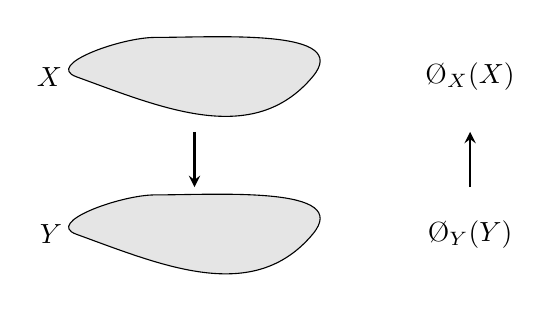
\begin{tikzpicture}
								\draw [fill=gray!20](0,0) to [out=-20,in=230] (3,0) to [out=50,in=0] (1,.5) to [out=180,in=160] (0,0) node [left,black]{$X\,$};
								\begin{scope}[yshift=-2cm]
									\draw [fill=gray!20](0,0) to [out=-20,in=230] (3,0) to [out=50,in=0] (1,.5) to [out=180,in=160] (0,0) node [left,black]{$Y\,$};
								\end{scope}
								\draw[-stealth,thick](1.5,-.7)--(1.5,-1.4);
								\node at (5,0) {$\O_X(X)$};
								\node at (5,-2) {$\O_Y(Y)$};
								\draw[-stealth,thick](5,-1.4)--(5,-.7);
							\end{tikzpicture}
						\end{center}
					\end{enumerate}
				\end{eg}

				Before we embark on scalar extensions, let us have a look at an alternative description of the module for K{\"a}hler differentials.
				Let $I_\Delta\subset S\otimes_RS$ be the kernel of the multiplication map defined by $\sum s_i\otimes t_i\mapsto \sum s_it_i$.

				\begin{lemma}
					The ideal $I_\Delta$ is generated by all $1\otimes s-s\otimes 1$ with $s\in S$. The map $\mathrm{d}:S\rightarrow I_{\Delta}/I^2_{\Delta}$ induced by $s\mapsto1\otimes s-s\otimes1$ is an $R$-linear derivation.
				\end{lemma}
				\begin{proof}\renewcommand{\qedsymbol}{}
					By direct computation.
				\end{proof}\renewcommand{\qedsymbol}{$\square$}
				
				The universal property of $\Omega_{S/R}$ then provides a natural $S$-module morphism $f:\Omega_{S/R}\rightarrow I_\Delta/I_\Delta^2$.

				\begin{prop}
					$\Omega_{S/R}\simeq I_\Delta/I_\Delta^2$.
				\end{prop}

				Assume that $R\rightarrow S\rightarrow T$ are ring morphisms.

				\begin{prop}(Cotangent sequence)
					There is a natural exact sequence of $T$-modules
					\begin{equation*}
						\begin{tikzcd}[row sep=tiny,
							/tikz/column 1/.append style={nodes={text width=5em, text centered}},
							/tikz/column 2/.append style={nodes={text width=2.5em, text centered}},
							/tikz/column 3/.append style={nodes={text width=2.5em, text centered}}]
							T\otimes_S\Omega_{S/R}\ar[r] & \Omega_{T/R}\ar[r] & \Omega_{T/S}\ar[r] & 0\\
							& \mathrm{d}t\ar[r,mapsto] & \mathrm{d}t &\\
							t\otimes \mathrm{d}s\ar[r,mapsto] & t\mathrm{d}s & &
						\end{tikzcd}
					\end{equation*}
				\end{prop}

				\noindent Think: $\Omega_{T/R}$ relative cotangent space.

				\begin{prop}\label{prop--conormal-sequence}
					If $T=S/J$ there is a natural exact sequence of $T$-modules 
					\begin{equation*}
						\begin{tikzcd}[row sep=tiny,
							/tikz/column 1/.append style={nodes={text width=2.5em, text centered}},
							/tikz/column 2/.append style={nodes={text width=5em, text centered}},
							/tikz/column 3/.append style={nodes={text width=2.5em, text centered}}]
							J/J^2\ar[r,"\delta"] & T\otimes_S\Omega_{S/R}\ar[r] & \Omega_{T/R}\ar[r] & 0\\
							& t\otimes\mathrm{d}s \ar[r,mapsto] & t\mathrm{d}s &\\
							j\ar[r,mapsto] & 1\otimes \mathrm{d}j & &
						\end{tikzcd}
					\end{equation*}
					If $R=K$ and $m\subset S$ a maximal ideal with $T=S/m\simeq K$, then the above sequence becomes 
					\begin{equation*}
						\begin{tikzcd}
							m/m^2\ar[r,"\delta"] & K\otimes_S\Omega_{S/K}\ar[r] & \Omega_{K/K}\ar[r] & 0
						\end{tikzcd}
					\end{equation*}
					and $\delta$ defines an isomorphism $m/m^2\simeq K\otimes_S\Omega_{S/K}$ (as $\Omega_{K/K}=\{0\}$, $\delta$ is obviously surjective; injectivity from derived long exact sequence).
				\end{prop}

				If $f:U\rightarrow V$ is a morpshim of affine varieties, we write $\Omega_{U/V}$ for $\Omega_{\O_U(U)/\O_V(V)}$.
				\\

				\noindent If $f:X\rightarrow Y$ is a map of algebraic varietes, there is a sheaf $\Omega_{X/Y}$ of $\O_X$-modules obtained by glueing together all $\Omega_{U/V}$, with $U\subset X$ and $V\subset Y$ affine open.
				\\

				\noindent If $X$ and $Y$ are smooth, irreducible curves and $f:X\rightarrow Y$ is separable, then the cotangent sequence is exact:
				\begin{equation*}
					\begin{tikzcd}
						0\ar[r] & f^\ast\Omega_{Y/K}\ar[r] & \Omega_{X/K}\ar[r] & \Omega_{X/Y}\ar[r] & 0.
					\end{tikzcd}
				\end{equation*}
				This is used to prove Riemann-Hurwitz. Hence, we need to understand sheaves of modules.

				{\color{gray}\subsubsection*{Comments on Riemann-Hurwitz and Differentials:}

					\noindent From \autoref{prop--kahlerdiff-universal} we know that $\Omega_{S/R}$ satisfies the universal property.

					\begin{exc}
						Show that $S=R/J$ $\Longrightarrow$ $\Omega_{S/R}=0$.
					\end{exc}

					\begin{exc}
						Show that if $R=K$ is a field, $S=L$ a separable extension $\Longrightarrow$ $\Omega_{L/K}=0$.
					\end{exc}

					\begin{exc}
						Show that $S^\prime\otimes_S\Omega_{S/R}\simeq\Omega_{S^\prime/R^\prime}$ where $S^\prime=R^\prime\otimes_RS$.
					\end{exc}
				
					\noindent Cotangent sequence: Intuition
					
					\begin{center}
						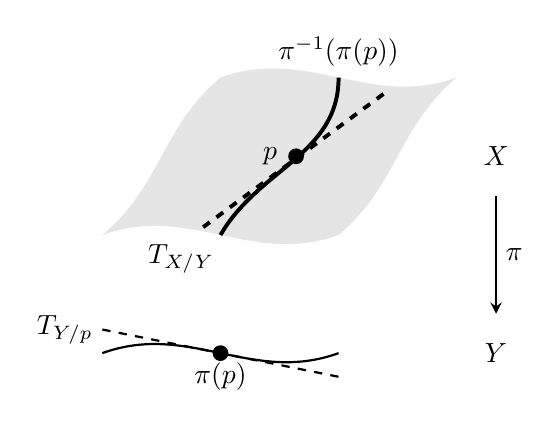
\begin{tikzpicture}
							\fill[gray!20](0,0) to [out=40,in=220] (1.5,2) to [out=20,in=200] (4.5,2) to [out=220,in=40] (3,0) to [out=200,in=20] (0,0);
							\draw[line width=.05cm,black](1.5,0) to [out=60,in=270] (3,2) node [above]{$\pi^{-1}(\pi(p))$};
							\fill[black] (2.46,1) circle [radius=.1cm] node [left]{$p\,\,$};
							\draw[line width=.05cm,dashed,black] (1.28,.1)--(3.65,1.85);
							\node at (1,0) [below,black]{$T_{X/Y}$};
							\draw[thick,black](0,-1.5) to [out=20,in=200] (3,-1.5);
							\fill[black] (1.5,-1.5) circle [radius=.1cm] node [below]{$\pi(p)$};
							\draw[thick,dashed,black] (0,-1.2)--(3,-1.8);
							\node at (0,-1.2) [left,black]{$T_{Y/p}$};
							\node at (5,-1.5) [black]{$Y$};
							\node at (5,1) [black]{$X$};
							\draw[-stealth,thick,black](5,.5)--(5,-1);
							\node at (5,-.25) [right,black]{$\pi$};
						\end{tikzpicture}
					\end{center}

					\begin{equation*}
						\begin{tikzcd}[/tikz/column 4/.append style={nodes={anchor=base west}}]
							0\ar[r] & T_{X/Y}\ar[r] & T_{X/p}\ar[r] & \pi^\ast T_{Y/p}\\
							0 & \Omega_{X/Y}\ar[l] & \Omega_{X/p}\ar[l] & \pi^\ast\Omega_{Y/p}\ar[l]\\
							0 & \Omega_{T/S}\ar[l] & \Omega_{T/R}\ar[l] & T\otimes\Omega_{S/R}\ar[l]
						\end{tikzcd}
					\end{equation*}
					with $R=\O_p(p)$, $S=\O_Y(Y)$ and $T=\O_X(X)$. Connection to previous definition of cotangent space: $m/m^2\simeq K\otimes_S\Omega_{S/K}$, $R=K$, $S$ local ring at point $p$, $m$ maximal ideal, $S/m\simeq K$.
					\\

					\noindent\underline{NB}: It might be fruitful to think of $\pi$ as a principal bundle and the cotangent sequence as being similar (in spirit) to the exact sequence
					\begin{equation*}
						\begin{tikzcd}
							0\ar[r] & VX\ar[r] & TX\ar[r] & \pi^\ast TY\ar[r] & 0
						\end{tikzcd}
					\end{equation*}
					of the tangent bundle of the principal bundle $X$ over the base $Y$ with vertical subspace $VX$; if the sequence splits (upon choosing a connection), $\pi^\ast TY$ is the horizontal subspace and $TX=VX\oplus
					\pi^\ast TY$.
				}



	\section{Schemes}

		So far we have studied algebraic varieties over an algebraically closed field, finitely generated and without nilpotents and having only closed points. With schemes we can eliminate the need of a base field. It provides a broad, robust framework and has better algebaic/functorial properties.
		
		\subsection{Affine Schemes}

			Let $R$ be a unital, commutative ring.

			\begin{defi}(Affine scheme)
				The affine scheme associated to $R$ or the spectrum of $R$ is the set $\spec R$ of all prime ideals of $R$.
			\end{defi}

			\begin{eg}
				\begin{enumerate}
					\item $R=K[X]=\O_X(X)$, the coordinat ring of an affine variety over $K=\bar{K}$. Then $\spec R$ is the affine scheme associated to $X$. Note that $X=\msp R\subset\spec R$. E.g. embedded in $\AA^n$, $(a_1,
					dots,a_n)\leftrightarrow (x_1-a_1,\dots,x_n-a_n)$, then $\spec R=\{\text{points}\}\cup\{\text{irreducible subvarieties}\}$.
					\item $\spec K[T]$: have maximal ideals $(T-\lambda)$, $\lambda\in K$ but also prime ideal $(0)$.
					\item $\spec\Z=\{(p)|p\text{ prime}\}\cup\{(0)\}$.
				\end{enumerate}
			\end{eg}

			Idea: For varieties over $K=\bar{K}$, we defined regular functions $f:\msp R\rightarrow K$. Note that $K\simeq R/m$ for any $m
			\in\msp R$ and $\O_X(X)=R$.

			\begin{defi}
				Let $X=\spec R$ and $P\in X$.
				\begin{enumerate}
					\item The residue field $\kappa(P)$ of $X$ at $P$ is the field of fractions of $R/P$.
					\item If $f\in R$, then the value $f(P)$ of $f$ at $P$ is the image of $f$ under $R\rightarrow R/P\rightarrow\kappa(P)$.
				\end{enumerate}
			\end{defi}

			\begin{eg}
				\begin{enumerate}
					\item $R=\O_X(X)$. $X$ affine variety over $K=\bar{K}$ then 
						\begin{equation*}
							\kappa(P)=\begin{cases}
							K,& \text{if $P$ maximal}\\
							K(Y),&\text{if $P=I(Y)$ irreducible}
							\end{cases}
						\end{equation*}
					\item $R=\Z$. Take e.g. $f=7$, $P=(5)$ then $f(P)=7(5)=2\in\Z/5\Z$.
				\end{enumerate}
			\end{eg}

			\begin{defi}
				Let $X=\spec R$. The zero locus of a set $S\subset R$ is
				\begin{equation}
					V(S)=\{P\in X|\forall f\in S:f(P)=0\}=\{P\in X|S\subset P\}.
				\end{equation}
			\end{defi}

			\begin{defi}
				The ideal of a set $Y\subset X$ is
				\begin{equation}
					I(Y)=\{f\in R|\forall P\in Y:f(P)=0\}=\bigcap_{P\in Y}P.
				\end{equation}
			\end{defi}

			With the above definitions we obtain a version of the Nullstellensatz similar to the case of varieties:

			\begin{thm}
				(Nullstellensatz for Schemes)\\ The maps $V$ and $I$ are mutually inverse, inclusion-reversing bijections between zero loci in $X$ and radical ideals in $R$. 
			\end{thm}
			\begin{proof}\renewcommand{\qedsymbol}{}
				Left as an exercise, use fact that $\bigcap_{P\in\spec R: J\subset P}P=\sqrt{J}$.
			\end{proof}\renewcommand{\qedsymbol}{$\square$}

			Let $X=\spec R$. As for varieties,
			\begin{enumerate}
				\item $\emptyset=V(1)$, $X=V(0)$
				\item $V(S)\cup V(S^\prime)=V(SS^\prime)$
				\item $\bigcap_{i\in I}V(S_i)=V(\bigcup_{i\in I}S_i)$
			\end{enumerate}

			\begin{defi}
				The Zariski topology on $X$ is the topology whose closed sets are the sets $V(S)$ with $S\subset R$.
			\end{defi}

			\begin{prop}
				The principal open subsets $U_f=X\backslash V(f)=\{P\in X|f\notin P\}$ with $f\in R$ form a base of the Zariski topology on $X$.
			\end{prop}
			\begin{proof}
				See Example Sheet 2, example 1.
			\end{proof}

			\noindent\underline{NB}: Note that not all points in $X$ are closed. A point $P\in X$ is closed if and only if $P $ is a maximal ideal ($\bar{\{P\}}=V(P)=\{P^\prime\in\spec R|P\subset P^\prime\}$). Non-closed points are called generic points.

			\begin{eg}
				
				\begin{enumerate}
					\item Consider scheme associated to variety $X$, then have closed points which are the actual points in $X$ and the generic points which are actually irreducible subvarieties of $X$.
					\item $R=\Z$, then $(p)$ ($p$ prime) are closed while $(0)$ is generic. If $f\in\Z$, then $f((p))=f\modd p$ while $f((0))=f\in\Q$ 
				\end{enumerate}
			\end{eg}

			Now let us endow the affine scheme with a structure sheaf.
			Let $X=\spec R$. Our goal is to define the structure sheaf $\O_X$ making $X$ into a ringed space. We need to define regular functions on $U\subset X$ into a field that varies with $P\in U$. This can be done in two ways:
			\begin{enumerate}
				\item define local regular functions on each open $U\subset X$
				\item define regular functions on principal open sets and glue
			\end{enumerate}

			\noindent We follow the first way and then check that on principal open subsets we get the functions we would expect.
			We would like to have some key properties:
			\begin{enumerate}
				\item $\O_X(U_f)\simeq R_f$ for all $f\in R$
				\item $\O_{X,P}\simeq R_P$ making $(X,\O_X)$ into a locally ringed space (i.e. stalks are local rings)
			\end{enumerate}

			\noindent Let $U\subset X=\spec R$ be open.

			\begin{defi}
				A regular function $\phi$ on $U$ is a family $(\phi_P)_{P\in U}$ with $\phi_P\in R_P$, such that there are $f,g\in R$ satisfying $f\notin Q$ and $\phi_Q=\frac{g}{f}\in R_Q$ for all $Q$ in a neighbourhood of $P$ in $U$. The set of all regular functions on $U$ is denoted $\O_X(U)$.
			\end{defi}

			\begin{prop}
				The construct $\O_X$ is a sheaf of rings on $X$.
			\end{prop}

			The sheaf $\O_X$ is the structure sheaf of $X$.

			\begin{prop}\label{prop--principal}(Regular functions on principal open subsets)
				Let $X=\spec R$. For any $f\in R$, $\O_X(U_f)\simeq R_f$.
			\end{prop}
			\begin{proof}
				An isomorphism $R_f\rightarrow \O_X(U_f)$ is given by $\frac{g}{f^r}\mapsto\phi$ with $\phi_P=\frac{g}{f^r}$ ($r\in\N$) for all $P\in U_f$. Ring morphism and injectivity is straightforward to check. Surjectivity is not so intuitive, proof is similar to the variety-case: shrinking the neighbourhood can assume that it contains a principal open set $U_h$ and show that in fact $h=f$ (see [G1] Proposition 12.20 for the full proof).
			\end{proof}

			\begin{cor}
				$\O_X(X)\simeq R$.
			\end{cor}
			\begin{proof}
				It is $X=U_1$ and $R_1=R$.
			\end{proof}

			\begin{prop}\label{prop--germs}(Germs of regular functions)
				For any $P\in X$, $\O_{X,P}\simeq R_P$.
			\end{prop}
			\begin{proof}
				An isomorphism $\O_{X,P}\rightarrow R_P$ is given by $\overline{(U,\phi)}\mapsto\phi_P$. Details are left as an exercise (see [G1] Lemma 12.18 for the proof).
			\end{proof}

			We now take a moment to think about what $\O_X$ means. If $\phi\in\O_X(U)$ and $P\in U$, then the image of $\phi_P$ under $R_P\rightarrow R_P/P_P\hookrightarrow\kappa(P)$ is well-defined and denoted $\phi(P)$.
			\\

			Warning: A regular function is in general not determined by its values $f(P)$ at all $P$ as the following example shows.

			\begin{eg}(Fat point)
				Let $R=K[T]/(T^2)$, $K$ field, $X=\spec R$, $\O_X(X)\simeq R=\{a+bT|a,b\in K\}$. Then $X=\{(T)\}$, $\phi\in\O_X(X)$ with $\phi((T))=a$. Hence, $a+bT$ and $a+b^\prime T$ have same evaluation under $\phi$.
			\end{eg}

			So far, we have defined the set $\spec R$ with its Zariski topology and structure sheaf $\O_{\spec R}$. An affine scheme is a locally ringed space of the form $(\spec R,\O_{\spec R})$ for some ring $R$.

			\begin{defi}
				A scheme is a locally ringed space $(X,\O_X)$ that has an open cover by affine schemes, $X=\bigcup_{i\in I}U_i$ such that $U_i=\spec R_i$ and $\O_X|_{U_i}=\O_{\spec R_i}$.
			\end{defi}

			\begin{remark}
				\begin{enumerate}
					\item In the french school of algebraic geometry, this is sometimes called a prescheme (similar to our earlier definition of prevarieties).
					\item The cover need not be finite.
				\end{enumerate}
			\end{remark}

			\subsubsection*{Morphisms and Functors}

				Problem: A morphism $f:X\rightarrow Y$ of varieties has a well-defined pullback $f^\ast:\O_Y\rightarrow\O_X$ (by precomposition). Moreover, $(f^\ast)^{-1}(I_p)=I_{f(p)}$ for all $p\in X$. This is not given when working with schemes.

				\begin{defi}\label{def--scheme-morphism}(Morphism of schemes)
					A morphism of locally ringed spaces $(X,\O_X)\rightarrow(Y,\O_Y)$ is
					\begin{enumerate}
						\item a continuous map $f:X\rightarrow Y$ and
						\item a map of sheaves $f^\ast:\O_Y\rightarrow\O_X$ compatible with $f$, i.e. for each $V\subset Y$ have $f^\ast_V:\O_Y(V)\rightarrow\O_X(f^{-1}(V))$ ring morphism such that for all $V\subset W\subset Y$,
						\begin{equation*}
							\begin{tikzcd}[/tikz/column 1/.append style={nodes={text width=6em, text centered}},
								/tikz/column 2/.append style={nodes={text width=6em, text centered}}]
								\O_Y(W)\ar[r,"|_{V}"]\ar[d,"f^\ast_W"] & \O_Y(V)\ar[d,"f^\ast_V"]\\
								\O_X(f^{-1}(W))\ar[r,"|_{f^{-1}(V)}"] & \O_X(f^{-1}(V))
							\end{tikzcd}
						\end{equation*}
						commutes and the $f^\ast$-preimage of $I_P\subset\O_{X,P}$ is $I_{f(P)}\subset\O_{Y,f(P)}$.
					\end{enumerate}
				\end{defi}

				Schemes form a category where the morphisms are the morphisms of locally ringed spaces.

				\begin{prop}
					The assignment $f\mapsto f^\ast$ defines a bijection between ringed space morphisms $\spec S\rightarrow\spec R$ and ring morphisms $R\rightarrow S$.
				\end{prop}
				\begin{proof}
					The above are constructed such that for $f:X\rightarrow Y$, have 
					\begin{equation*}
						\begin{tikzcd}[row sep=tiny]
							f^\ast:\O_{\spec R}(\spec R)\ar[r]\ar[d,equal] & \O_{\spec S}(\spec S)\ar[d,equal]\\
							R & S
						\end{tikzcd}.
					\end{equation*}
					Conversely, given $\phi:R\rightarrow S$, define $f:\spec S\rightarrow\spec R, P\mapsto\phi^{-1}(P)$. This is morphism of schemes, since $f^{-1}(V(J))=\{P\in\spec S|\phi^{-1}(P)\supset J\}=\{P\in\spec S|P\supset\phi(J)\}=V(\phi(J))$ which is closed, i.e. $f$ continuous. Now need morphism of sheafs. For this define $\phi_P:R_{\phi^{-1}(P)}\rightarrow S_P$ for all $P\in\spec S$, which in turn defines map $f^\ast_U:\O_{\spec R}(U)\rightarrow\O_{\spec S}(f^{-1}(U)),(\psi_Q)_{Q\in U}\overset{\phi_Q}{\mapsto}(\phi_Q(\psi_Q))$. Left to check that these two constructions are mutually inverse.
				\end{proof} 

				\begin{cor}
					There is a category equivalence
					\begin{equation*}
						\begin{tikzcd}
							\{\text{affine schemes}\}\ar[r,shift left=.5ex,"F"] & \ar[l,shift left=.5ex,"\spec"]\{\text{unital, commutative rings}\}
						\end{tikzcd}
					\end{equation*}
				\end{cor}

				Having established the functoriality statements above one might think about an embedding of the category of schemes into a category of functors: Every scheme $X$ defines a contravariant functor
				\begin{equation*}
					h_X:\mathrm{Schemes}\rightarrow\mathrm{Sets},\, T\mapsto X(T):=\Hom(T,X).
				\end{equation*}
				Such a functor is called representable (it is represented by $X$).

				\begin{lemma}
					(Yoneda) Morphisms $X\rightarrow Y$ of schemes correspond bijectively to natural transformations $h_X\rightarrow h_Y$.
				\end{lemma}

				This works as follows: given $f:X\rightarrow Y$, have $\alpha_f:\Hom(T,X)\rightarrow\Hom(T,Y),\phi\mapsto f\circ\phi$. Given $\alpha_X:\Hom(X,X)\rightarrow\Hom(X,Y),\id_X\mapsto\alpha_X(\id_X)$. Can check that these constructions are mutually inverse.
				
				\begin{remark}
					$h_X$ is determined by its restrictions to affine schemes. Thus, $X$ is determined by a family of all $X(S):=X(\spec S)$.
				\end{remark}

				\begin{eg}
					Consider $X=\{x|x^2=2\}$. Then $X(\Z)=\{z\in\Z|z^2=2\}=\emptyset$, $X(\Q),X(\R)\dots$.
				\end{eg}

				\begin{cor}
					Each affine scheme $X=\spec R$ defines a covariant functor
					\begin{equation*}
						h^\prime_X:\mathrm{Rings}\rightarrow\mathrm{Sets},\, S\mapsto X(S):=\Hom(R,S).
					\end{equation*}
					The assignment $X\mapsto h^\prime_X$ is an equivalence onto a subcategory.
				\end{cor}


				{\color{gray}\subsubsection*{Comments on (affine) schemes:}
				
					Differences to varieties:
					\begin{enumerate}
						\item Non-closed fields: $\spec \R[T]$ contains elements of the form $(T-a)_{a\in\R}$, $(0)$ and $(p(T))_{\deg p=2}$ with $p$ irreducible polynomial; $(0)$ is prime but not maximal.
						\item Why prime ideals? Take e.g. $\spec\Z[T]$, then $(T)$ prime but not maximal ($\Z\simeq\Z[T]/(T)$ is not a field).
						\item A scheme is not determined by its points. Consider e.g. $R=K[T]/(T^2)$ (dual numbers): $\spec R=\{(T)\}\overset{1:1}{\longleftrightarrow}\spec K=\{(0)\}$. In general, $\spec R=\spec R/\sqrt{(0)}$ as a set! In the literature one often writes $|X|=X$ as just a set/topological space.
						\item Non-closed points $P\in\spec R\backslash\msp R$: Consider e.g. $R=\O_V(V)$ with $R=\CC[S,T]/(T(T-1))$ and $V=\{(x,y)\in\CC^2|y(y-1)=0\}$ disjoint union of two lines. Closed points are maximal ideals, i.e. points $(x,y)$ with $y=0$ or $y=1$.The prime ideal $(T)$ is a non-closed point:
						\begin{align*}
							\bar{(T)}=&\{P\in\spec R|(T)\subset P\}\\
							=&\{(T),\text{maximal ideals corresponding to }(x,0)\text{ with fixed }x\}\\
							=&\text{line and all closed points in it}.
						\end{align*}
					\end{enumerate}

					\begin{defi}
						(Fat points) An $n$-fold point (fat point) of a scheme $X$ over a field $K=\bar{K}$ is a $K$-scheme $\spec R$ that has one point such that $\dim_KR=n$.
						\begin{equation*}
							\begin{tikzcd}
								\spec R\ar[d] & R\\
								\spec K & K\ar[u]
							\end{tikzcd}
						\end{equation*}
					\end{defi}

					\begin{exc}
						Show that
						\begin{enumerate}
							\item any double point is isomorphic to $\spec K[T]/(T^2)$,
							\item not all triple points are isomorphic.
						\end{enumerate}
					\end{exc}

					\begin{exc}
						\begin{enumerate}
							\item If $X=\spec R$, where $R$ is the coordinate ring of an affine variety $V$ over $K=\bar{K}$ ($X$ scheme associated to $V$), show that the set of closed points is dense in $X$ with respect to the Zariski topology.
							\item Give an example of a scheme $X$ where the set of closed points is not dense in $X$.\\(Ex.: $\CC[T]/(T)\simeq\CC$ one point $(0)$ maximal ideal.)
							\item Is there an irreducible affine scheme $X=\spec R$ with $R$ not an integral domain?
							\item Are there rings $R,S$, $R\subset S$ but $\dim\spec R>\dim\spec S$?
							\item Is there an affine scheme $X=\spec R$ of dimension one having exactly two points?
						\end{enumerate}
					\end{exc}
				
				}


		\subsection{Constructions on Schemes}

			Recall: An affine sceme is a locally ringed space of the form $\spec R$ for a ring $R$. A scheme is a locally ringed space admitting an open cover by affine schemes. Thus, an (affine) scheme is a topological space with a structure sheaf. Equivalently: a representable functor (view $\spec R$ as $\Hom_\text{Rings}(R,-)$).
			\\

			Beware: The underlying space is a weak concept: different schemes may have homeomorphic spaces. This is why a functor, rather than one Hom-set is needed. As a consequence, when defining subschemes, embeddings etc., set-theoretic constructions are inadequate.

			\begin{defi}
				Let $X$ be a scheme. An open subscheme of $X$ is an open subset $U\subset X$ endowed with the structure sheaf $\O_U=\O_X|_U$.
			\end{defi}

			\noindent\underline{NB}: This is well-defined scheme with a morphism $\iota:U\rightarrow X$.
			\\

			Hence, open subspaces naturally inherit a scheme structure. In order to define closed subschemes, we need to be more careful.

			\begin{defi}
				Let $X=\spec R$. An affine subscheme of $X$ is an affine scheme $Y=\spec S$ with a morphism $\iota:Y\rightarrow X$ such that $\iota^\ast:R\rightarrow S$ is surjective.
			\end{defi}

			Hence, affine subschemes correspond to quotient rings (cf. subvarieties: $\O_Y(Y)=\O_X(X)/I_X(Y)$).

			\begin{prop}
				The assignment $J\mapsto\spec R/J$ defines a bijection between ideals in $R$ and affine subschemes of $X$.
			\end{prop}

			\begin{eg}
				Consider $R=K[T]$, $J_1=(T)$. Then $R/J_1\simeq K$. For $J_2=(T^2)$ have $R/J_2\simeq K[T]/(T^2)$ which has the same underlying set but is different algebraically.
			\end{eg}

			\begin{defi}
				Let $X=\spec R$ and $J,J^\prime\subset R$ be ideals. The union of $\spec R/J$ and $\spec R/J^\prime$ is an affine subscheme $\spec R/(J\cap J^\prime)$. The intersection of $\spec R/J$ and $\spec R/J^\prime$ is the affine subscheme $\spec R/(J+J^\prime)$.
			\end{defi}

			\noindent\underline{NB}: The intersection corresponds to the ideal $J+J^\prime$, rather than $\sqrt{J+J^\prime}$ which would be expected from the Nullstellensatz.

			\begin{eg}
				Consider $R=K[S,T]$ with $J=(T)$, $J^\prime=(T-S^2)$. Then $R/(J+J^\prime)\simeq K[S]/(S^2)$ (cf. $R/\sqrt{J+J^\prime}\simeq K[S]/(S)$).
			\end{eg}

			We now want to define closed subschemes, having previously defined closed affine subschemes.

			\begin{defi}
				Let $X$ be any scheme. A closed subscheme of $X$ is a scheme $Y$ with morphism $\iota:Y\rightarrow X$ such that $\iota|_{\iota^{-1}(U)}:\iota^{-1}(U)\rightarrow U$ is an affine subscheme for each affine open $U\subset X$.
			\end{defi}	 

			\begin{remark}
				\begin{enumerate}
					\item Enough to check $\iota|_{\iota^{-1}(U)}$ on a fixed open cover.
					\item This suggests that closed subschemes correspond to \qt{sheaves of ideals}.
				\end{enumerate}
			\end{remark}

			\begin{remark}(Glueing schemes)
				Similarly to  varieties, schemes can be glued:
				\begin{enumerate}
					\item Given schemes $\{X_i\}_{i\in I}$ with open subsets $U_{ij}\subset X_i$ and isomorphisms $f_{ij}:U_{ij}\rightarrow U_{ji}$ for all $i,j\in I$ satisfying $f^{-1}_{ij}=f_{ji}$ and $f_{jk}\circ f_{ij}=f_{ik}$ on $U_{ij}\cap f^{-1}_{ij}(U_{jk})\subset U_{ik}$ for all distinct $i,j,k\in I$.
					\item Set $X=(\bigsqcup_{i\in I}X_i)/\sim$, where $\sim$ is the equivalence relation defined by $x\sim y:\Longleftrightarrow y=f_{ij}(x)$. Have natural maps $\iota_i:X_i\rightarrow X, x\mapsto\bar{x}$.
					\item Topologise $X$ by declaring $U\subset X$ open if $\iota^{-1}_i(U)\subset X_i$ is open for all $i\in I$.
					\item Ring $X$ by defining a structure sheaf $\O_X$ as the unique sheaf of rings on $X$ with $\O_X|_{U_i}\simeq\O_{U_i}$ via isomorphisms compatible with the $f_{ij}$.
				\end{enumerate}
			\end{remark}

			\begin{eg}
				A set with an open cover by affine schemes.
			\end{eg}

			We can now associate schemes not only to affine varieties but also to prevarieties as follows: Let $X$ be a prevariety over a field $K=\bar{K}$. The set $X_\mathrm{sch}$ of all irreducible closed subsets of $X$ is a scheme, obtained by gluing the affine schemes $\spec \O_{U_i}(U_i)$ for an open cover of $X$ by affine varieties $U_i$. $X_\mathrm{sch}$ is the scheme associted to $X$.

			\begin{prop}
				The open subsets of $X_\mathrm{sch}$ are precisely the open sets of $X$ and $\O_{X_\mathrm{sch}}(U)=\O_X(U)$ for any open $U$. Moreover, any morphism of prevarieties $f:X\rightarrow Y$ naturally induces a morphism $f_\mathrm{sch}:X_\mathrm{sch}\rightarrow Y_\mathrm{sch}$ of schemes.
			\end{prop}

			\subsubsection*{Relative Viewpoint}

				Problem: In many situations, we want to study schemes over a fixed base, with morphisms over this base. Algebraically, this corresponds to the difference between rings and $K$-algebras.

				\begin{defi}
					Let $Y$ be any scheme. A scheme over $Y$ or $Y$-scheme is a scheme $X$ with a morphism $f:X\rightarrow Y$. If $f:X\rightarrow Y$ and $f^\prime:X^\prime\rightarrow Y$ are $Y$-schemes, then a morphism of $Y$-schemes from $X$ to $X^\prime$ is a morphism of schemes $g:X\rightarrow X^\prime$ with $f=f^\prime\circ g$, i.e. we have a commutative diagram
					\begin{equation*}
						\begin{tikzcd}
							X\ar[r,"f"]\ar[d,"g"'] & Y\\
							X^\prime\ar[ru,"f^\prime"'] &
						\end{tikzcd}						
					\end{equation*}
				\end{defi}

				If $Y=\spec S$, then a scheme over $Y$ is referred to as a scheme over $S$. An affine scheme $\spec R$ over an affine base $\spec S$ corresponds to an $S$-algebra.

				\noindent\underline{NB}: Every scheme is a $\spec\Z$-scheme.

				\begin{eg}
					$\spec \O_X(X)$ for a variety $X$ over $K$.
				\end{eg}

				\begin{remark}
					Consider $X=\spec\Z[T]$, $Y=\spec\Z[T]/(p(T))$ for some polynomial $p$. $X,Y$ are schemes over $\Z$.
					\begin{enumerate}
						\item Evaluate at any $\Z$-algebra $R$: $Y(R)=\Hom(Y,R)\longleftrightarrow\{x\in R|p(x)=0\}$.
						\item Base change: $Y\times_{\spec\Z}\spec\Q=:Y_\Q$ is the $\Q$-scheme (scheme over $\spec\Q$) defined by $Y_\Q=\spec\Q[T]/(p(T))$.
						\item More generally,
						\begin{equation*}
							\spec A\times_{\spec B}\spec C\simeq\spec(A\otimes_BC).
						\end{equation*}
					\end{enumerate}
				\end{remark}

				\begin{defi}
					Let $f_i:X_i\rightarrow Y$ be two schemes over a scheme $Y$. A fibre product of $X_1$ and $X_2$ over $Y$ is a scheme $P$ with morphisms such that
					\begin{equation*}
						\begin{tikzcd}
							P\ar[r,"\pi_2"]\ar[d,"\pi_1"] & X_2\ar[d,"f_2"]\\
							X_1\ar[r,"f_1"] & Y
						\end{tikzcd}
					\end{equation*}
					commutes and satisfies a universal property. We write $X_1\times_YX_2$ for the fibre product.
				\end{defi}

				\begin{prop}
					The fibre product of any two schemes $X_1,X_2$ over $Y$ exists and is unique up to a unique isomorphism.
				\end{prop}
				\begin{proof}
					Uniqueness follows immediately from universal property. As for existence, start from the affine case, $Y=\spec S$, $X_i=\spec R_i$ ($X_i$ scheme over $Y$, i.e. $R_i$ is an $S$-algebra). Then take $\spec(R_1\otimes_SR_2)=P$. The general case is obtained by glueing. 
				\end{proof}

				\begin{defi}(Intersection)
					Let $X_1$ and $X_2$ be closed subschemes of a scheme $X$. The (scheme-theoretic) intersection $X_1\cap X_2$ is the fibre product $X_1\times_XX_2$ with its natural $X$-scheme structure.
				\end{defi}

				\begin{defi}(Scheme of finite type)
					A $Y$-scheme $f:X\rightarrow Y$ is of finite type over $Y$ if $Y$ admits an open cover $U_i=\spec(R_i)$ such that $f^{-1}(U_i)$ has a finite cover by spectra of finitely generated $R_i$-algebras.
				\end{defi}

				\begin{eg}
					Schemes of finite type over a field $K$.
				\end{eg}

				\begin{defi}(Reduced scheme)
					A scheme $X$ is called reduced if for any open $U\subset X$, $\O_X(U)$ has no nilpotent elements.
				\end{defi}

				\begin{prop}
					Let $K$ be an algebraically closed field. The maps $X\mapsto X_\mathrm{sch}$ and $f\mapsto f_\mathrm{sch}$ define an isomorphism of categories from prevarieties over $K$ to reduced schemes of finite type over $K$.
				\end{prop}

				A prevariety over $K$ is viewed as a reduced scheme of finite type over $K$. A point is understood as a closed point and a morphism as a morphism over $K$.

				\begin{defi}(Separated scheme)
					A scheme $X$ over $Y$ is separated if the image of the diagonal morphism $X\rightarrow X\times_YX,x\mapsto(x,x)$ is closed.
				\end{defi}

				\begin{cor}
					The maps $X\mapsto X_\mathrm{sch}$ and $f\mapsto f_\mathrm{sch}$ define an isomorphism of categories from varieties over $K$ to separated reduced schemes of finite type over $K$.
				\end{cor}

				Thus, a variety over $K $ is a separated reduced scheme of finite type over $K$.
				
		
		

	\section{Sheaves}

		\subsection{Sheaves of Modules}

			As a general observation in algebra, having an algebraic object (e.g. a field, ring etc.) one can define an action of this object an another algebraic object with a milder structure (vector spaces, modules etc.). In this spirit, we now want to study sheaves of modules over schemes. These are the analogues of this philosphy for schemes. Algebraically, the idea is to obtain some sort of sheaf on which the structure sheaf of a scheme acts.

			Geometrically, we want to consider modules that vary along a curve/variety/scheme: If $X$ is a scheme, then $\O_X(U)$ is a ring for each open $U\subset X$. It is natural to study objects that are modules over $\O_X(U)$ in a \qt{coherent} way.

			\begin{eg}
				Tangent spaces (give tangent sheaves), vector spaces (give vector bundles), ideals (give ideal sheaves).
			\end{eg}

			\begin{defi}(Sheaf of $\O_X$-modules)
				Let $X$ be a scheme. A (pre)sheaf of modules over $X$ or (pre)sheaf of $\O_X$-modules is a (pre)sheaf $\M$ on $X$ such that
				\begin{enumerate}
					\item $\M(U)$ is an $\O_X(U)$-module for each $U$
					\item for any open $U\subset V\subset X$ and $a,b\in\M(V)$, $\lambda\in\O_X(V)$:
						\begin{equation*}
							(a+b)|_U=a|_U+b|_U,\qquad (\lambda a)|_U=\lambda|_U\,a|_U. 
						\end{equation*}
				\end{enumerate}
			\end{defi}

			\noindent\underline{NB}: Note that although (ii) in the definition above suggests that the restrictions are module morphisms, this is not actually the case since $\M(U)$ and $\M(V)$ are modules over different rings ($\O_X(U)$ and $\O_X(V)$).

			\begin{defi}(Morphism of sheaves of $\O_X$-modules)
				A morphism $f:\M\rightarrow\mathcal{N}$ of (pre)sheaves of $\O_X$-modules consists of an $\O_X(U)$-module morphism $f_U:\M(U)\rightarrow\mathcal{N}(U)$ for each open $U\subset X$, compatible with restrictions (i.e. there is a commutative diagram).
			\end{defi}

			\noindent\underline{NB}: The definition above says that morphisms are natural transformations between sheaves viewed as functors.
			\\

			\noindent A sheaf of $\O_X$-modules is called an $\O_X$-module (can think of it as a module over the whole sheaf of rings).

			\begin{eg}
				Simple examples are $\O_X$ itself (rings are modules) and the trivial module $\M(U)=0$. 
			\end{eg}

			Let $X$ and $Y$ be schemes and $f:X\rightarrow Y$ a continuous map (not necessarily a morphism). We want to view $\O_X$-modules as $\O_Y$-modules in order to be able to compare them in one framework.

			\begin{defi}(Pushforward of sheaves)
				The pushforward of a (pre)sheaf $\M$ on $X$ is the (pre)sheaf $f_\ast\M$ on $Y$ defined by 
				\begin{equation*}
					(f_\ast\M)(U)=\M(f^{-1}(U)).
				\end{equation*}
			\end{defi}

			\begin{remark}
				\begin{enumerate}
					\item If $\M$ is an $\O_X$-module, then $f_\ast\M$ is an $\O_Y$-module.
					\item The definition of scheme morphisms in \autoref{def--scheme-morphism} looks quite elaborate. With the definition above, we can formulate a simpler version: it is a continuous function $f:X\rightarrow Y$ with a sheaf morphism $f^\ast:\O_Y\rightarrow f_\ast\O_X$ with $(f^\ast_P)^{-1}(I_P)=I_{f(P)}$.
				\end{enumerate}
			\end{remark}

			\begin{eg}(Twisting sheaves)
				Consider $\P^n$ over $K=\bar{K}$. We define the twisting sheaf $\O_{\P^n}(d)$ with $d\in\Z$ by
				\begin{equation*}
					\O_{\P^n}(d)(U)=\{\frac{g}{f}|f,g\in K[T_0,\dots,T_n]\text{ homogeneous, }\deg g-\deg f=d,f(P)\neq0\text{ on }U\}.
				\end{equation*}
				\begin{enumerate}
					\item This defines a sheaf of $\O_{\P^n}$-modules on $\P^n$ for each $d\in\Z$: the quotients $\frac{g}{f}$ come from the quotient field of $K[T_0,\dots,T_n]$ and the restrictions are just the identity maps; if two such quotients agree on intersections, then they come from something global, i.e. they are the same everywhere. The $\O_{\P^n}$-module structure comes from the form of elements in $\O_{\P^n}$ which is such that they preserve $\deg g-\deg f$ under multiplication.
					\item We have $\O_{\P^n}(0)=\O_{\P^n}$.
					\item $\O_{\P^n}(-1)$ is isomorphic to the tautological sheaf $\mathcal{T}$ on $\P^n$:
						\begin{equation*}
							\mathcal{T}(U)=\{\phi:U\rightarrow\AA^{n+1}|\forall P\in U:\phi(P)\in P\}.
						\end{equation*}
						What is $\mathcal{T}$? It is the set of maps mappiing each point in $\P^n$ to the line in $\AA^{n+1}$ it defines as an equivalence class. In this sense it is the most natural sheaf over projective space. 
				\end{enumerate}
			\end{eg}

			\begin{eg}\label{ex--skyscraper}
				(Skyscraper sheaf) Consider the inclusion $\iota:P\rightarrow X$ of a point $P\in X$ into the variety $X$. Then $\O_P(P)=K$ and $\O_P(\emptyset)=\{0\}$. The pushforward to $X$ is obtained as
				\begin{equation*}
					(\iota_\ast\O_P)(U)=\O_P(\iota^{-1}(U))=\begin{cases}
						K, & \text{for }P\in U\\
						\{0\}, & \text{for }P\notin U
					\end{cases}
				\end{equation*}
				for all open subsets $U\subset X$. Hence, the morphism $\O_Y\rightarrow\iota_\ast\O_P,\,\phi\mapsto\iota^\ast\phi$ is just evaluation of $\phi$ on $U\subset X$ at $P$ (if $P\in U$).\\
				\begin{center}
					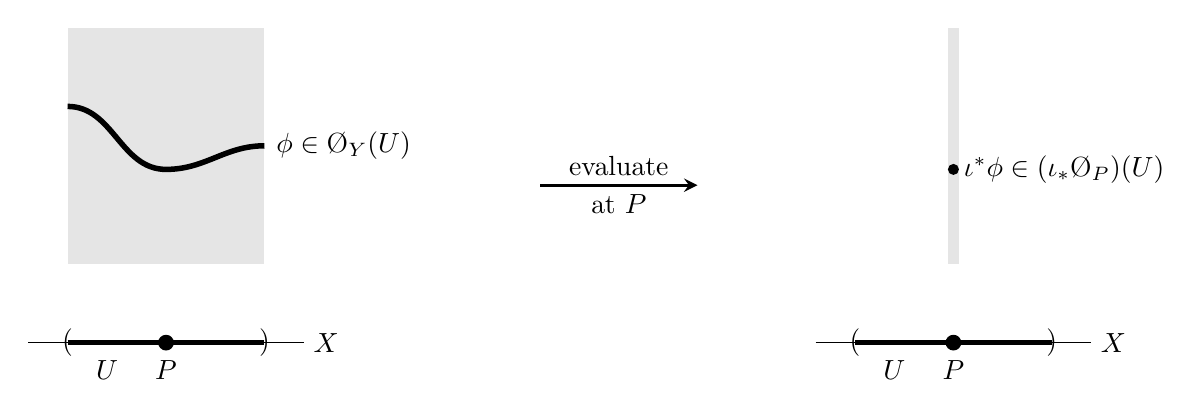
\begin{tikzpicture}
						\fill[gray!20](0,0)--(0,3)--(2.5,3)--(2.5,0)--cycle;
						\draw[line width=.07cm](0,2) to [out=0,in=180](1.25,1.2) to [out=0,in=180](2.5,1.5) node [right]{$\phi\in\O_Y(U)$};
						\draw (-.5,-1)--(3,-1) node [right]{$X$};
						\draw[line width=.07cm](0,-1) node {(} --(2.5,-1) node {)};
						\fill (1.25,-1) circle [radius=.1cm];
						\node at (1.25,-1.1) [below]{$P$};
						\node at (.5,-1.1) [below]{$U$};
						\draw[-stealth,line width=.04cm](6,1)--(8,1);
						\node at (7,1) [above]{evaluate};
						\node at (7,1) [below]{at $P$};
						\begin{scope}[xshift=10cm]
							\draw (-.5,-1)--(3,-1) node [right]{$X$};
							\draw[line width=.07cm](0,-1) node {(} --(2.5,-1) node {)};
							\fill (1.25,-1) circle [radius=.1cm];
							\node at (1.25,-1.1) [below]{$P$};
							\node at (.5,-1.1) [below]{$U$};
							\fill[gray!20](1.18,0)--(1.18,3)--(1.32,3)--(1.32,0)--cycle;
							\fill (1.25,1.2) circle [radius=.07cm];
							\node at (1.26,1.2) [right]{$\iota^\ast\phi\in(\iota_\ast\O_P)(U)$};
						\end{scope}
					\end{tikzpicture}
				\end{center}
				Sections of $\iota_\ast\O_P$ can thus be seen as functions on $X$ that only take a value at $P$. We usually write $K_P:=\iota_\ast\O_P$ and call this the skyscraper sheaf on $X$ at $P$ (the naming should become apparent from the picture above).
			\end{eg}


		\subsection{Constructions on Sheaves of Modules}

			Let $\M$ and $\mathcal{N}$ be two sheaves of modules over a scheme $X$, and $f:\M\rightarrow\mathcal{N}$ a morphism.

			\begin{prop}
				(Kernel sheaf) The contruction
				\begin{equation*}
					(\ker f)(U)=\ker(f_U:\M(U)\rightarrow\mathcal{N}(U))
				\end{equation*}
				defines a sheaf of $\O_X$-modules.
			\end{prop}
			\begin{proof}
				It is clear that the kernel of each $f_U$ is a module, and since $f$ is compatible with restrictions $\ker f$ is a presheaf of modules. What is left to show is that it is a sheaf. Let $\{U_i\}_{i\in I}$ be an open cover of $U$ and let $m_i\in(\ker f)(U_i)\subset\M(U_i)$. It is $f_{U_i}(m_i)=0$ by definition. Since $\M$ is a sheaf, there exists $m\in\M(U)$ such that $m|_{U_i}=m_i$ for all $i\in I$. We need to show $f_U(m)=0$. But as $\mathcal{N}$ is a sheaf, it is enough to show $f_{U_i}(m|_{U_i})=0$ which follows at once from $f_{U_i}(m_i)=0$ for all $i\in I$.
			\end{proof}

			\noindent\underline{NB}: The result of $\ker f$ being in fact a sheaf is expected since the property of being sent to zero is a local property.

			\begin{prop}
				(Image presheaf) The construction 
				\begin{equation*}
					(\im^\prime f)(U)=\im(f_U:\M(U)\rightarrow\mathcal{N}(U))
				\end{equation*}
				defines a presheaf of $\O_X$-modules.
			\end{prop}

			\noindent Note that $\im^\prime f$ is not in general a sheaf. In order to see this, consider an open cover $\{U_i\}$ of $U$. If $n_i\in(\im^\prime f)(U_i)$ then $n_i=f_{U_i}(m_i)$ for some $m_i\in\M(U_i)$. However, there is no reason to expect $f_{U_i}(m_i)$ for all $i\in I$ to glue together to the image of one and the same $m\in\M(U)$. Hence, in general, $n\neq f_U(m)$.
			Let us look at a concrete example of this observation.

			\begin{eg}
				Consider $\iota:\AA^1\rightarrow\AA^2,x_1\mapsto(x_1,0)$ with $\iota^\ast:\O_{\AA^2}\rightarrow\O_{\AA^1}, p(x_1,x_2)\mapsto p(x_1,0)$ and open sets $U=\AA^2\backslash\{(0,0)\}$, $U_{1,2}=\{(x_1,x_2)\in\AA^2|x_{1,2}\neq0\}$. Then $U_1\cap U_2=\{(x_1,x_2)|x_1,x_2\neq0\}$. Now $f(U)=K[x_1]$, $f(U_1)=K[x_1]_{x_1}$, $f(U_2)=\{0\}$ and $f(U_1\cap U_2)=\{0\}$ (localisation with respect to $0$ gives $\{0\}$). Both, $\frac{1}{x_1}\in f(U_1)$ and $0\in f(U_2)$ agree on $f(U_1\cap U_2)$ (as it is the trivial module) but they do not give rise to the same global function.   
			\end{eg}

			Since $\im^\prime f$ is in general only a presheaf, but we prefer to work with sheaves if possible, one might wonder if there is some way to turn $\im^\prime f$ into a sheaf while staying as close as possible to its original definition. We answer this question positively in the next section, introducing the concept of sheafification.

			As for the image presheaf, its sheafification $\im f$ is called the image sheaf of $f$.

			\begin{defi}
				(Injective and surjective morphisms) A morphism $f:\M\rightarrow\mathcal{N}$ is called injective if $\ker f$ is trivial and surjective if $\im f\simeq\mathcal{N}$.
			\end{defi}

			\noindent\underline{NB}: Being injective implies $\M(U)\hookrightarrow\mathcal{N}(U)$. The implication of surjectivity is obscured by sheafification and can not be written down in such a nice way.

			\begin{defi}
				(Quotient sheaf) If $f:\M\rightarrow\mathcal{N}$ is injective, then $\M(U)$ is a submodule of $\mathcal{N}(U)$ for all $U$. The quotient sheaf $\mathcal{N}/\M$ is the sheafification of the presheaf $u\mapsto\mathcal{N}(U)/\M(U)$.
			\end{defi}

			\begin{defi}
				(Dual sheaf) The dual sheaf $\M^\vee$ is the sheafification of the presheaf $U\mapsto\Hom_{\O_X(U)}(\M(U),\O_X(U))$.
			\end{defi}

			\begin{defi}
				(Exact sequence) An exact sequence of sheaves of modules over $X$ is a sequence
				\begin{equation*}
					\begin{tikzcd}
						\dots\ar[r] & \M_{i-1}\ar[r,"f_{i-1}"] & \M_i\ar[r,"f_i"] & \M_{i+1}\ar[r] & \dots
					\end{tikzcd}
				\end{equation*}
				where for each $i$, $\im f_{i-1}\simeq\ker f_{i}$.
			\end{defi}

			\noindent\underline{NB}: The above definition basically contains two requirements. First, $f_{i+1}\circ f_i=0$. This implies (exercise) existence of a morphism from $\phi^\prime:\im^\prime f_i\rightarrow\ker f_{i+1}$ by direct construction. But every morphism from a presheaf to a sheaf defines a unique morphism from the sheafification of the presheaf to the sheaf; hence, we obtain $\phi:\im f_i\rightarrow\ker f_{i+1}$ from $\phi^\prime$ (note that $\phi^\prime$ is just the inclusion, via $f_{i+1}\circ f_i=0$, hence easy to construct). As a second requirement, this last morphism has to be an isomorphism.
			
			\begin{remark}\label{rem--exact-sequence}
				Exactness is equivalent to either exactness on all open subsets, exactness on an open cover or exactness on all stalks.
			\end{remark}

			\begin{defi}
				(Direct sum) Let $\M$ and $\mathcal{N}$ be two sheaves of modules over a scheme $X$. Then
				\begin{equation*}
					(M\oplus\mathcal{N})(U)=\M(U)\oplus\mathcal{N}(U)
				\end{equation*}
				defines a sheaf of $\O_X$-modules.
			\end{defi}

			\noindent\underline{NB}: This does not require any sheafification. For $\{U_i\}$ some open cover of $U\subset X$ with $m_i\in\M(U_i)$ and $n_i\in\mathcal{N}(U_i)$, $m_i\oplus n_i$ can be glued to $m\oplus n\in(\M\oplus\mathcal{N})(U)$ simply by glueing the $m_i$ to $m$ and $n_i$ to $n$ on the sheaves $\M$ and $\mathcal{N}$, respectively.

			\begin{defi}
				(Tensor product) Let $\M$ and $\mathcal{N}$ be two sheaves of modules over a scheme $X$. Then
				\begin{equation*}
					(\M\otimes^\prime\mathcal{N})(U)=\M(U)\otimes_{\O_X(U)}\mathcal{N}(U)
				\end{equation*}
				defines a presheaf of $\O_X$-modules.
			\end{defi}

			In general, $\M\otimes^\prime\mathcal{N}$ is not a sheaf. Its sheafification is called the tensor product $\M\otimes\mathcal{N}$.
			That $\M\otimes^\prime\mathcal{N}$ is not a sheaf can be seen from the following example.

			\begin{eg}
				Let $X=\P^1$, $\M=\O_{\P^1}(1)$ and $\mathcal{N}=\O_{\P^1}(-1)$. Take open sets $U_i=\{[x_0:x_1]|x_i\neq0\}\subset X$. Then $x_i\otimes\frac{1}{x_i}\in(\M\otimes^\prime\mathcal{N})(U_i)$ for $i=0,1$ agree on the overlap:
				\begin{equation*}
					x_0\otimes\frac{1}{x_0}=x_0\frac{x_1}{x_0}\otimes\frac{x_0}{x_1}\frac{1}{x_0}=x_1\otimes\frac{1}{x_1}.
				\end{equation*}
				But, globally, $\mathcal{N}(\P^1)=\{0\}$ (otherwise there would be elements of the form $\frac{g}{f}$ with $g$ of lower degree than $f$ which do not exist globally on $\P^1$). Hence, the two elements above cannot be glued to a global section.
			\end{eg}

		
		\subsection{Sheafification}

			We saw in the previous section that not all constructions on sheaves yield a sheaf again. However, every such construction gives a presheaf that can be turned into a sheaf which resembles its properties \qt{as closely as possible} via a standard procedure called sheafification.

			\begin{defi}
				(Sheafification) Let $\F^\prime$ be a presheaf on a scheme $X$. For $U\subset X$ open we set
				\begin{equation*}
					\F(U)=\{(\phi_P)_{P\in U}|\forall P\in U:\phi_P\in\F^\prime_P\text{ and }(\ast)\}
				\end{equation*}
				where $(\ast)$ for all $P\in U$ there is an open neighbourhood $U_P\in U$ and $s\in\F^\prime(U)$ such that for all $Q\in U_P$, $\phi_Q=s_Q$ (with $s_Q\in\F^\prime_Q$ the germ of $s$ in $Q$). 
			\end{defi}

			Since this construction is of a local nature, $\F$ is a sheaf, called the sheafification of $\F^\prime$.
			
			\begin{eg}
				Consider the sheaf associated to the presheaf of constant functions on a topological space $X$.
				\begin{enumerate}
					\item There is a morphism $h:\F^\prime\rightarrow\F$ given by
						\begin{equation*}
							h_U:\F^\prime(U)\rightarrow\F(U),\sigma\mapsto(\sigma_P)_{P\in U}
						\end{equation*}
						for each open $U\subset X$.
					\item The morphism $h$ induces isomorphisms on stalks,
						\begin{align*}
							h_P:&\F^\prime_P\rightarrow\F_P,\sigma_P\mapsto\overline{(U,(\sigma_P)_{P\in U})},\\
							j_P:&\F_P\rightarrow\F^\prime_P,\overline{(U,\phi)}\mapsto\phi_P.
						\end{align*}
				\end{enumerate}
			\end{eg}

			\begin{remark}
				Any presheaf $\F^\prime$ on a scheme $X$ admits a natural morphism to its sheafification,
				\begin{equation*}
					\F^\prime(U)\rightarrow\F(U),\phi\mapsto(\phi_P)_{P\in U}
				\end{equation*}
				for all open subsets $U\subset X$.
			\end{remark}
			
			\begin{prop}
				A morphism $f:\F\rightarrow\mathcal{G}$ of sheaves is an isomorphism if and only if the induced map on each stalk is an isomorphism.
			\end{prop}
			\begin{proof}
				Let $f$ be an isomorphism. Then, clearly, $f_P$ is an isomorphism. Conversely, let $f_P$ isomorphism for all $P\in X$. It is enough to show that $f_U:\F(U)\rightarrow\mathcal{G}(U)$ is an isomorphism for $U\subset X$ open. 
				
				First, we show injectivity: For $\phi\in\F(U)$ assume $0=f(\phi)\in\mathcal{G}(U)$ $\Longrightarrow$ for all $P\in U$, $0=f(\phi)_P\in\mathcal{G}_P$. But $f_P$ injective $\Longrightarrow$ $\phi_P=0$. Hence, there is an open neighbourhood $U_P\subset U$ of $P$ where $\phi|_{U_P}=0$ for all $P\in U$. But $\F$ is a sheaf $\Longrightarrow$ $\phi=0$ in $\F(U)$.
				
				For surjectivity, consider $\psi\in\mathcal{G}(U)$. Let $\psi_P\in\mathcal{G}_P$ denote its germ for $P\in U$. As $f_P$ is surjective we find $\phi_P\in\F_P$ such that $f_P(\phi_P)=\psi_P$. We want to show that the $\phi_P$ give rise to a section $\phi\in\F(U)$. Assume that $\phi_P$ is represented by a section $\phi(P)$ in a neighbourhood $U_P\subset U$ of $P$. As $f(\phi(P))$ and $\psi|_{U_P}$ have the same germ at $P$, we may assume $f(\phi(P))=\psi|_{U_P}$ in $\mathcal{G}(U_P)$ (upon shrinking $U_P$ appropriately if necessary). Now consider $P,Q\in X$ and $\phi(P)\in\F(U_P),\phi(Q)\in\F(Q)$. Then $f(\phi(P))|_{U_P\cap U_Q}=\psi|_{U_P\cap U_Q}=f(\phi(Q))|_{U_P\cap U_Q}$ and injectivity proved above implies $\phi(P)|_{U_P\cap U_Q}=\phi(Q)|_{U_P\cap U_Q}$. Using the sheaf property we get $\phi\in\F(U)$ such that $\phi|_{U_P}=\phi(P)$ for all $P\in U$. Finally, $f(\phi)=\psi$ follows from the uniqueness of $\phi$ with the properties above.
			\end{proof}
			
			\begin{remark}
				This does not imply that isomorphic stalks of two sheaves give rise to the sheaves itselves being isomorphic.
			\end{remark}

			Let $h:\F^\prime\rightarrow\F$ be the morphism from $\F^\prime$ to its sheafification.

			\begin{cor}
				If $\F^\prime$ is a sheaf, then $\F\simeq\F^\prime$.
			\end{cor}

			\begin{prop}
				(Universal property) For any sheaf $\mathcal{G}$ and any morphism $f^\prime:\F^\prime\rightarrow\mathcal{G}$ there is a unique morphism $f:\F\rightarrow\mathcal{G}$ such that $f^\prime=f\circ h$, i.e.
				\begin{equation*}
					\begin{tikzcd}
						\F^\prime\ar[r,"h"]\ar[d,"f^\prime"] & \F\ar[dl,dashed,"f"]\\ \mathcal{G}
					\end{tikzcd}
				\end{equation*}
				commutes.
			\end{prop}
			\begin{proof}
				Let us first consider a more general situation where we have two presheaves $\F^\prime,\mathcal{H}^\prime$ with sheafifications $\F,\mathcal{H}$ such that 
				\begin{equation*}
					\begin{tikzcd}
						\F^\prime \ar[r,"h_{\F^\prime}"]\ar[d,"f^\prime"] & \F \ar[d,gray,"f"]\\
						\mathcal{H}^\prime \ar[r,"h_{\mathcal{H}^\prime}"] & \mathcal{H}
					\end{tikzcd}
				\end{equation*}
				where $f$ can be constructed as follows: At the level of open sets $U$, write $f_U:\F(U)\rightarrow\mathcal{H}(U)$. But these sections, by construction, are defined in terms of the stalks, $f_P:\F_P\rightarrow\mathcal{H}_P$. But these are precisley the stalks of the presheaves, so we can take $f_P=f^\prime_P:\F^\prime_P\rightarrow\mathcal{H}^\prime_P$. This gives rise to a well-defined $f$, obviously compatible with restrictions. Now take $\mathcal{H}^\prime$ to be the sheaf $\mathcal{G}$ in the proposition, then $h_{\mathcal{H}^\prime}$ is an isomorphism and we have proved existance of $f$ in the proposition. Uniqueness is left as an exercise.  
			\end{proof}

			\begin{eg}
				The structure sheaf $\O_X$ of an affine variety $X$ over a field $K=\bar{K}$ is the sheafification of the presheaf $\O_X^\prime$:
				\begin{equation*}
					\O^\prime_X(U)=\{\phi:U\rightarrow K|\exists f,g\in\O_X(X):\phi=\frac{g}{f}\}.
				\end{equation*}
			\end{eg}


		\subsection{Quasi-Coherent Sheaves}

			So far we have considered presheaves and sheaves of modules that are defined from modules over each open subset. One distinguished kind of such construction is obtained as follows. Consider $X=\spec R$ and $M\in$R-Mod. It turns out that from $M$ we can obtain a sheaf of modules by defining, on open sets, its localisations (as defined below).
			
			\begin{defi}
				(Localisation of modules) Let $R$ be a ring, $S\subset R$ multiplicatively closed and $M$ an $R$-module. The $S^{-1}R$-module $S^{-1}R\otimes_RM$ is called the localisation of $M$ at $S$, denoted $S^{-1}M$.
			\end{defi}

			\begin{remark}
				(Explicit construction) $S^{-1}M$ is the set of equivalence classes $\frac{m}{s}$ of $M\times S$ under the relation
				\begin{equation*}
					(m,s)\sim(m^\prime,s^\prime):\Longleftrightarrow\exists u\in S:u(ms^\prime-m^\prime s)=0
				\end{equation*}
				with $S^{-1}R$-module structure given by
				\begin{equation*}
					\frac{m}{s}+\frac{m^\prime}{s^\prime}=\frac{ms^\prime+m^\prime s}{ss^\prime},\qquad \frac{r}{s}\cdot\frac{m}{s^\prime}=\frac{rm}{ss^\prime}.
				\end{equation*}
				We use the notation $M_P$ and $M_a$ for localisation at prime ideals and sets $\{1,a,a^2,\dots\}$ as for rings.
			\end{remark}

			\noindent Idea: As stated earlier, we would like to construct sheaves associated to modules. We can now turn an $R$-module into a sheaf of modules over $\spec R$ whose stalks are the localisations $M_P$ of $M$.
			
			\begin{defi}
				(Sheaf associated to a module) Let $X=\spec R$ and $M$ an $R$-module. For each open $U\subset X$, $\widetilde{M}(U)$ is the set of all $(\phi_P)_{P\in U}$ with $\phi_P\in M_P$, such that for all $P\in U$ there are $f\in R,g\in M$ with 
				\begin{equation*}
					f\notin Q,\qquad\phi_Q=\frac{g}{f}\in M_Q
				\end{equation*}
				for all $Q$ in a neighbourhood of $P$ in $U$. The construct $\widetilde{M}$ is a sheaf of modules on $X$, called the sheaf associated to $M$. Note that $\widetilde{R}=\O_X$.
			\end{defi}

			\begin{remark}
				Observe that the definition above defines $\widetilde{R}$ just as a sheaf of modules. Hence, we do not have multiplication inside of its modules but we have multiplication with elements in $R$. In general, we need to specify how $\O_X$ acts on $\widetilde{M}(U)$. Now $\O_X(U)$ consists of elements $(\psi_P)$ which on the level of stalks are of the form $\frac{r}{s}$ with $r\in R$ and $s\in R\backslash P$ and act on $(\phi_P)$ by $\frac{r}{s}\cdot\frac{g}{f}$ (as we would expect).
			\end{remark}

			\begin{prop}\label{prop--module-sheaves}
				Let $X=\spec R$. Let $M,N,L$ be $R$-modules.
				\begin{enumerate}
					\item For each $P\in X$, $\widetilde{M}_P\simeq M_P$.
					\item For each $f\in R$, $\widetilde{M}(U_f)\simeq M_f$. In particular, for $f=1$, $\widetilde{M}(X)=M$. 
					\item Morphisms $\widetilde{M}\rightarrow\widetilde{N}$ correspond bijectively to module homomorphisms $M\rightarrow N$.
					\item The sequence \begin{tikzcd}[column sep=small]
						0\ar[r] & M\ar[r] & N\ar[r] & L\ar[r] & 0
					\end{tikzcd}
					of modules is exact if and only if the sequence \begin{tikzcd}[column sep=small]
						0\ar[r] & \widetilde{M}\ar[r] & \widetilde{N}\ar[r] & \widetilde{L}\ar[r] & 0
					\end{tikzcd}
					of associated sheaves is exact.
					\item $\widetilde{M\oplus N}\simeq\widetilde{M}\oplus\widetilde{N}$.
					\item $\widetilde{M\otimes N}\simeq\widetilde{M}\otimes\widetilde{N}$.
					\item $\widetilde{M^\vee}\simeq\widetilde{M}^\vee$.
				\end{enumerate}
			\end{prop}
			\begin{proof}\renewcommand{\qedsymbol}{}
				(Sketch) (i) and (ii) are proved analogous to \autoref{prop--principal} and \ref{prop--germs}.
				\begin{enumerate}
					\item[(iii)] Given $f:\widetilde{M}\rightarrow\widetilde{N}$ we get $f_X:M=\widetilde{M}(X)\rightarrow\widetilde{N}(X)=N$. Conversely, given $g:M\rightarrow N$, we can localise to $g_a:M_a\rightarrow N_a$ and gluing from the principal open subsets $U_a$ gives a global morphism. These two constructions are inverse to each other.
					\item[(iv)] This can be proved locally using two properties. First, a sequence of modules is exact if and only if its localisation at all prime ideals is exact (from commutative algebra). Second, a sequence of sheaves is exact if and only if it is exact on the level of stalks. The claim now follows from (i). 
				\end{enumerate}
				The proof of (v)-(vii) is left as an exercise.
			\end{proof}\renewcommand{\qedsymbol}{$\square$}
			
			With the construction above we have introduced a way of, given a module $M$, associating to it a sheaf $\widetilde{M}$. But we could also ask if, given a sheaf, can it be constructed from a module. If this is the case, it is called a quasi-coherent module.

			\begin{defi}
				(Quasi-coherent sheaf) Let $X$ be a scheme. A sheaf $\M$ of modules over $X$ is quasi-coherent if there is an open cover $\{U_i=\spec R_i\}$ of $X$ with $\M|_{U_i}\simeq\widetilde{M}_i$ for some $R_i$-module $M_i$.
			\end{defi}

			\noindent\underline{NB}: This vaguely reminds of local trivialisations of vector bundles in terms of its fibres (i.e. vector spaces).

			\begin{remark}
				\begin{enumerate}
					\item The restriction of a quasi-coherent sheaf to an affine open $U\subset X$ is of the form $\widetilde{M}$.
					\item Kernels, images, quotients, direct sums, tensor products and duals of quasi-coherent sheaves are quasi-coherent.
					\item Non-quasi-coherent examples exist (see below)
				\end{enumerate}
			\end{remark}

			\begin{eg}
				(Non-quasi-coherent sheaf) Take $X=\spec K[T]_{(T)}$ with points $(T), (0)$. The open sets are $X,\emptyset$ and $U=X\backslash\{(T)\}=\{(0)\}$. Now set $\mathcal{F}(X)=\mathcal{F}(\emptyset)=\{0\}$ and $\mathcal{F}(U)=K[T]_{(0)}=\O_X(U)$ with restriction maps the zero map. $\mathcal{F}$ is a sheaf of modules. However, the section at $U$ is non-trivial. But if $\mathcal{F}$ would be quasi-coherent it would be constructed from a non-zero module whereas $\mathcal{F}(X)$ is trivial. So if $\mathcal{F}$ was quasi-coherent, $\mathcal{F}(X)$ would have to be the non-trivial module \contradiction.
			\end{eg}

		
		\subsection{Ideal Sheaves and Pullbacks}
			
			\noindent Idea: Affine subvarieties and affine subschemes are vanishing sets of ideals. If $Z=\spec S$ is an affine subscheme of $X=\spec R$, then $S\simeq R/J$ for some ideal $J$, i.e. this ideal is defined by
			\begin{equation*}
				\begin{tikzcd}
					0\ar[r] & J\ar[r] & \O_X(X)\ar[r] & \O_Z(Z)\ar[r] & 0.
				\end{tikzcd}
			\end{equation*}
			Can we make this ideal global?

			\begin{defi}
				(Ideal sheaf) An ideal sheaf on a scheme $X$ is a sheaf $\J$ of modules on $X$ together with an injective morphism $\J\rightarrow\O_X$. Thus, $\J(U)$ is an ideal in $\O_X(U)$ for each open subset $U\subset X$.
			\end{defi}

			\begin{prop}\label{prop--ideal-sequence}
				Let $X$ be a scheme and $\iota:Z\rightarrow X$ a closed subscheme.
				\begin{enumerate}
					\item If a sheaf $\M$ on $Z$ is quasi-coherent, so is $\iota_\ast\M$ on $X$.
					\item The map $\iota^\ast$ induces an exact sequence 
						\begin{equation*}
							\begin{tikzcd}
								0\ar[r] & \J_{Z/X}\ar[r] & \O_X\ar[r,"\iota^\ast"] & \iota_\ast\O_Z\ar[r] & 0
							\end{tikzcd}
						\end{equation*}
						of quasi-coherent sheaves on $X$.
				\end{enumerate}
			\end{prop}
			\begin{proof}
				\begin{enumerate}
					\item Assume first $X=\spec R$. Then $Z$ is an affine subscheme $\spec R/J$ (as it is a closed subscheme). Now take a quasi-coherent sheaf $\M$ over $Z$, then $\M=\widetilde{M}$ for some $M\in R/J$-Mod. Now $\iota_\ast\M=\widetilde{M}$ with $M\in R$-Mod via $R\rightarrow R/J$. The general case is obtained by glueing.
					\item By (i) $\iota_\ast\O_Z$ is quasi-coherent and $\O_X$ also is quasi-coherent. Hence, if $\iota^\ast$ is surjective, its kernel will again be quasi-coherent and we can take it as $\J_{Z/X}$. Thus, it suffices to show surjectivity of $\iota^\ast$. First, assume $X=\spec R$ and hence $Z=\spec R/J$. Then $\O_X=\widetilde{R}$, $\iota_\ast\O_Z=\widetilde{R/J}$ and $\widetilde{R}\rightarrow\widetilde{R/J}$ is surjective since $R\rightarrow R/J$ is. The general case is obtained by glueing.
				\end{enumerate}
			\end{proof}

			\noindent The sheaf $\J_{Z/X}$ is the ideal sheaf of $Z$ in $X$.
			
			\begin{eg}
				(Skyscraper sequence) Consider $X=\P^1$ and $P=[1:0]\in\P^1$ with the inclusion $\iota:P\hookrightarrow X$. Then we have the skyscraper sequence
				\begin{equation*}
					\begin{tikzcd}
						0\ar[r] & \O_{X}(-1)\ar[r,"\cdot T_1"] & \O_X\ar[r,"g"] & K_P\ar[r] & 0
					\end{tikzcd}
				\end{equation*}
				with $g$ the evaluation at $P$ as in \autoref{ex--skyscraper}. This is an exact sequence. Injectivity of the first map is easy. Moreover, clearly $\im^\prime g=K_P$ (e.g. take the constant functions in $\O_X$) and as the evaluation at $P$ is a local condition, in fact $\im^\prime g$ is already a sheaf, i.e. $\im g=K_P$. Note that $\im^\prime f$ contains precisely the regular functions that vanish at $P$, i.e. it is already a sheaf (since this is a local condition). But
				\begin{equation*}
					(\im f)(U)=\{\phi\in\O_X(U)|\phi(P)=0\text{ if }P\in U\}=(\ker g)(U)
				\end{equation*}
				for all open $U\subset X$.
			\end{eg}
			
			\begin{remark}
				Any closed subscheme determines an ideal sheaf and vice versa. The first statement was proved above. For the second, consider the affine case again with an ideal sheaf $\J$. Then $\J(U_i)=J_i\subset\O_X(U_i)$ which gives us $\spec R/J_i$. The closed subscheme is obtained by glueing.
			\end{remark}

			Let $X,Y$ be schemes and $f:X\rightarrow Y$ a morphism. We want to pull back a quasi-coherent sheaf $\M$ on $Y$ to $X$.
			\\

			\noindent Idea (from affine case): If $X=\spec R,Y=\spec S$ and $M$ an $S$-module, then $R\otimes_SM$ is an $R$-module: given $f:X\rightarrow Y$ we get $f^\ast:S=\O_Y(Y)\rightarrow\O_X(X)=R$, i.e. an $S$-action on $R$. Thus, for $\M=\widetilde{M}$, we define the pullback $f^\ast\M$ of $\M$ along $Y$ by $f^\ast\M=\widetilde{R\otimes_SM}$.
			\\
			
			\noindent The construction for the general case involves some technical necessities.

			
			\begin{defi}\label{def--pullback-sheaves}(Pullback of a sheaf)
				\begin{enumerate}
					\item We would like to write for open $U\subset X$ something like $\M(f(U))$. However, $f(U)$ is not, in general, an open subset of $Y$. Insetad, we adapt the definition of stalks of $\M$ to open sets $U\subset X$ and consider the sheafification $f^{-1}\M$ of the presheaf given by 
						\begin{equation*}
							U\mapsto\{(V,\phi)|V\subset Y\text{ open, }f(U)\subset V,\phi\in\M(V)\}/\sim
						\end{equation*}
						where $(V,\phi)\sim(V^\prime,\phi^\prime):\Longleftrightarrow\exists W$ open, $f(U)\subset W\subset V\cap V^\prime$: $\phi|_W=\phi^\prime|_W$. On the level of stalks of this presheaf, and hence the sheafification $f^{-1}\M$, we get $f^{-1}\M_P=\M_{f(P)}$ as expected. 
					\item $f^{-1}\M$ still has a $\O_Y$-module structure. We obtain the desired $\O_X$-module structure by tensoring: $f^\ast\M=\O_X\otimes_{f^{-1}\O_Y}f^{-1}\M$ with $f^\ast\M(U)=\O_X(U)\otimes_{f^{-1}\O_Y(U)}f^{-1}\M(u)$ (where the tensor product is again understood to be the sheafification).
					
					In the affine setting we recover (a): 
					\begin{align*}
						(f^\ast\M)_P&=\O_{X,P}\otimes_{(f^{-1}\O_{Y,P})}(f^{-1}\M)_P=R_P\otimes_{\O_{Y,f(P)}}M_{f(P)}=R_P\otimes_{S_{f(P)}}M_{f(P)}\\
						&=(R\otimes_SM)_P
					\end{align*}
					with the last equality following from a standard result in commutative algebra.
				\end{enumerate}
			\end{defi}

			\noindent\underline{NB}: For practical purposes it is usually sufficient to work locally were the simple affine construction is sufficient.

			\begin{eg}
				\begin{enumerate}
					\item If $f:X\rightarrow Y$, then $f^\ast\O_Y=\O_X\otimes_{f^{-1}\O_Y}f^{-1}\O_Y\simeq\O_X$.
					\item If $\iota:P\rightarrow X$ is the inclusion of a closed point, then $\iota^\ast\M$ has a unique non-trivial section space $\iota^\ast\M(P)$ over $\kappa(P)$ (residue field): the fibre of $\M$ at $P$. If $X=\spec R$ and $\M=\widetilde{M}$, then $\iota^\ast\M(P)=M/PM$.
				\end{enumerate}
			\end{eg}

			\begin{prop}
				Let $\iota:Z\rightarrow X$ be the inclusion of a closed subscheme.
				\begin{enumerate}
					\item $\iota^\ast\iota_\ast\mathcal{N}\simeq\mathcal{N}$ for quasi-coherent $\mathcal{N}$ on $Z$.
					\item $\iota_\ast\iota^\ast\M\simeq(\iota_\ast\O_Z)\otimes_{\O_X}\M$ for quasi-coherent $\M$ on $X$. More generally, $\iota_\ast(\mathcal{N}\otimes\iota^\ast\M)\simeq(\iota_\ast\mathcal{N})\otimes\M$.
				\end{enumerate}
			\end{prop}
			\begin{proof}
				According to our previous results, it suffices to prove these isomorphisms locally, i.e. in the affine setting. Let $X=\spec R$, $Z=\spec R/J$ and $\mathcal{N}=\widetilde{N}$, $\M=\widetilde{M}$. By \autoref{prop--module-sheaves} it further suffices to show the isomorphisms on the level of the modules associated to the respective sheaves. We recall that the pushforward is given by viewing an $R/J$-module as an $R$-module and from the affine case of \autoref{def--pullback-sheaves} that the pullback is obtained by tensoring with $R$ over $R/J$.
				\begin{enumerate}
					\item The $R/J$-module $R/J\otimes_R N$ is naturally isomorphic to $N$ (from commutative algebra).
					\item The $R$-module $N\otimes_{R/J}(R/J\otimes_RM)$ is naturally isomorphic to the $R$-module $N\otimes_RM$ (from commutative algebra, using associativity of tensor product).
				\end{enumerate}
			\end{proof}


		\subsection{Vector Bundles}

			\noindent Let $X$ be a scheme.
			
			\begin{defi}(Locally free sheaf of modules)
				A sheaf of modules on $X$ is locally free if there is an open cover $\{U_i=\spec R_i\}$ of $X$ with $\M|_{U_i}\simeq\widetilde{M}_i$ for some free $R_i$-module $M_i$ of finite rank. It is further of constant rank $\rank\M=r$ if all $M_i$ have rank $r$.
			\end{defi}

			\begin{remark}
				\begin{enumerate}
					\item It need not hold that for every open $U\subset X$, $\M|_U\simeq\widetilde{M}$ with $M$ a free $\O_X(U)$-module of finite rank (cf. local trivialisations w.r.t. open cover of base). E.g. take $X=\spec(K\times K)$ ($K=\bar{K}$ field) and consider the module $K\times\{0\}$. This is not a free module over $K\times K$ but its restrictions to each open set are free.
					\item Fibres are finite-dimensional vector spaces (over the respective residue field).  
				\end{enumerate}
			\end{remark}

			\begin{defi}
				(Vector bundle) Locally free sheaves are called vector bundles. Locally free sheaves of constant rank 1 are called line bundles.
			\end{defi}

			\begin{eg}
				Let $X$ be a scheme.
				\begin{enumerate}
					\item The structure sheaf $\O_X$ is a line bundle (it gives $\O_X(U)$ over $\O_X(U)$).
					\item If $\M$ and $\mathcal{N}$ are locally free $\O_X$-modules of rank $m$ and $n$, respectively, then $\M\oplus\mathcal{N}$, $\M\otimes\mathcal{N}$ and $\M^\vee$ are locally free of rank $m+n$, $mn$ and $m$, respectively. (This can be checked by taking an open cover where they \qt{trivialise}, i.e. they are associated to modules $M$ and $N$. Then the result follows from linear algebra on free modules.)
					\item If $f:Y\rightarrow X$ is a morphism, then $f^\ast\M$ is a locally free $Y$-module of rank $m$. This is not, in general, true for the pushforward of a morphism.
					\item If $X$ is a closed subscheme of $\P^n$, then the twisting sheaf $\O_X(d):=\iota^\ast\O_{\P^n}(d)$ is a line bundle. (The pullback of a line bundle is a line bundle. That $\O_{\P^n}(d)$ is a line bundle can be seen as follows: as per usual, cover $\P^n$ by $U_i=\{[x_0:\ldots:x_n]|x_i\neq0\}$. Now we can multiply by $x_i^d$ in order to obtain locally $\O_{\P^n}(d)(U)\simeq\O_{\P^n}(0)(U)$. But the condition for being a line bundle is local and $\O_{\P^n}(0)(U)=\O_{\P^n}(U)$.)
				\end{enumerate}
			\end{eg}

			\begin{prop}
				Let $\begin{tikzcd}[column sep=small]
					0\ar[r] & \M_1\ar[r] & \M_2\ar[r] & \M_3\ar[r] & 0
				\end{tikzcd}$ be an exact sequence of quasi-coherent sheaves on a scheme $X$.
				\begin{enumerate}
					\item If $\M$ is quasi-coherent, then 
					\begin{equation*}
						\begin{tikzcd}
							0\ar[r] & \M_1\otimes\M\ar[r] & \M_2\otimes\M\ar[r] & \M_3\otimes\M\ar[r] & 0
						\end{tikzcd}
					\end{equation*} 
					is exact whenever $\M$ or each $\M_i$ is locally free (in general, tensoring is not exact; it is right-exact).
					\item If $f:Y\rightarrow X$ is a morphism, then 
					\begin{equation*}
						\begin{tikzcd}
							0\ar[r] & f^\ast\M_1\ar[r] & f^\ast\M_2\ar[r] & f^\ast\M_3\ar[r] & 0
						\end{tikzcd}
					\end{equation*}
					is exact whenever each $\M_i$ is locally free. (This, as per usual, can be seen easily on the level of modules.)
				\end{enumerate}
			\end{prop}

			In \autoref{sec--smooth-varieties} we already saw tangent spaces of a variety and they turned out give useful information about the variety, like its smoothness. However, rather than studying the tangent space at each point individually like we did before, it is more appropriate to view those as the fibres of a tangent sheaf. We describe this point of view in the following.
			\\

			\noindent Recall: The module of K{\"a}hler differentials of the algebra $S$ over the ring $R$ is the pair $(\Omega_{S/R},\mathrm{d})$, where
			\begin{enumerate}
				\item $\Omega_{S/R}$ is the $S$-module generated by the symbols $\mathrm{d}s$ for $s\in S$, subject to the relations $\mathrm{d}(s+t)=\mathrm{d}s+\mathrm{d}t$, $\mathrm{d}(st)=s\mathrm{d}t+t\mathrm{d}s$ and $\mathrm{d}r=0$ for all $s,t\in S$ and $r\in R$.
				\item $\mathrm{d}:S\rightarrow\Omega_{S/R}$ is defined by $s\mapsto\mathrm{d}s$.
			\end{enumerate}
			Also recall the universal property of $\Omega_{S/R}$.
			\\

			\noindent In \autoref{subsec--differentials} we also gave an alternative description of K{\"a}hler differentials as $\Omega_{S/R}\simeq I_\Delta/I_\Delta^2$, where $I_\Delta\subset S\otimes_RS$ is the kernel of the multiplication map $S\otimes_RS\rightarrow S$.
			\\

			\noindent Idea: Define the cotangent sheaf $\Omega_{X/T}$ of a separated scheme $X$ over a scheme $T$ by replacing $I_\Delta$ by the appropriate ideal sheaf.

			\begin{defi}
				(Conormal sheaf) If $\iota:X\rightarrow Y$ is a closed embedding with corresponding ideal sheaf $\J$, then the quasi-coherent sheaf $\J/\J^2$ is called the conormal sheaf of embedding $\iota$. 
			\end{defi}

			\noindent\underline{NB}: The conormal sheaf is again quasi-coherent. We have seen that $\J$ and quotients thereof are quasi-coherent, thus we need to show that $\J^2$ is. But on affine patches, $\J^2$ corresponds to ideals of the form $J^2$.

			\begin{defi}
				(Relative cotangent sheaf) The relative cotangent sheaf $\Omega_{X/T}$ is the pullback of the conormal sheaf of the diagonal embedding $X\rightarrow X\times_T X$.
			\end{defi}

			\noindent Let us unpack this definition. Consider the diagonal embedding $\iota:X\rightarrow X\times_TX,a\mapsto(a,a)$. Since $X$ is separated, this is a closed embedding, i.e. it correpsonds to an ideal sheaf $\J_{X/X\times_TX}$. This is an ideal sheaf over the fibre product, thus, $\J/\J^2$ will still be a sheaf over the fibre product. In order to obtain a sheaf over $X$ we simply pull back along, $\iota^\ast(\J/\J^2)$. 

			In the affine setting with $X=\spec S$ and $T=\spec R$ the diagonal map corresponds precisely to multiplication $S\otimes_RS\rightarrow S,a\otimes b\mapsto ab$; the ideal sheaf $\J$ corresponds to the ideal $I_\Delta$. Hence, we recover the earlier definition.
			
			\begin{defi}
				(Relative tangent sheaf) The relative tangent sheaf is the dual sheaf $(\Omega_{X/T})^\vee$ of the relative cotangent sheaf.
			\end{defi}

			Let $X$ be a variety of pure dimension $n$ over $K=\bar{K}$ (then $\Omega_X=\Omega_{X/\spec K}$ restricts to $\widetilde{\Omega}_{R_i/K}$ on an open cover $\{U_i=\spec R_i\}$).

			\begin{thm}
				(Smoothness criterion)\\ $X$ is smooth if and only if $\Omega_X$ is locally free of rank $n$.
			\end{thm}
			\begin{proof}
				Both conditions are local, so it suffices to prove the statement above on an open cover. Assume $X=\spec R\subset\AA^r$ with $R=\K[r]/I(X)$ and $I(X)=(f_1,\dots,f_m)$ for some $m,r\in\N$. If we take $P\in X$ then the fibre of $\Omega_X$ at $P$ is obtained as
				\begin{equation*}
					\Omega_R\otimes_RR/P=(K\mathrm{d}x_1\oplus\dots\oplus K\mathrm{d}x_r)/(\sum_{j=1}^r\frac{\mathrm{d}f_i}{\mathrm{d}x_j}(P)\mathrm{d}x_j)=(T_PX)^\vee.
				\end{equation*} 
				\begin{enumerate}
					\item [``$\Leftarrow$'':] If $\Omega_X$ is locally free of rank $n$, then $\dim T_PX=n$. Hence, $X$ is smooth at $P$. But $P$ was chosen arbitrarily, hence $X$ is smooth.
					\item [``$\Rightarrow$'':] Assume that $X$ is smooth at $P$. Then $\rank(\frac{\mathrm{d}f_i}{\mathrm{d}x_j}(P))_{i,j}=r-n$. This implies that, w.l.o.g., $\mathrm{d}x_1,\dots,\mathrm{d}x_n$ generate $(T_PX)^\vee$, i.e. the submatrix of the Jacobian given by the last $r-n$ rows and columns has non-vanishing determinant. But this is an open condition, i.e. at every point $Q$ in an open neighbourhood $U\subset X$ of $P$, $\mathrm{d}x_1,\dots,\mathrm{d}x_n$ generate $(T_QX)^\vee$. Hence, $\dim(T_QX)^\vee\le n$ and from \autoref{prop--smoothness}, $\dim(T_QX)^\vee=n$, i.e. $\mathrm{d}x_1,\dots,\mathrm{d}x_n$ is in fact a basis. Therefore, we can write
					\begin{equation*}
						\Omega_X|_U=\O_U\mathrm{d}x_1\oplus\dots\oplus\O_U\mathrm{d}x_n
					\end{equation*}
					which shows that $\O_X$ is indeed locally free.
				\end{enumerate}
			\end{proof}

			Recall that in \autoref{prop--conormal-sequence} we have introduced the conormal sequence. We can now globalise this sequence appropriately.

			\begin{prop}
				If $Y$ is a variety over $K$ and $\iota:X\rightarrow Y$ a closed embedding with ideal sheaf $\J$, then there is an exact sequence
				\begin{equation*}
					\begin{tikzcd}
						\J/\J^2\ar[r] & \iota^\ast\Omega_{Y/K}\ar[r] & \Omega_{X/K}\ar[r] & 0
					\end{tikzcd}
				\end{equation*}
				of sheaves on $X$.
			\end{prop}

			\begin{remark}
				\begin{enumerate}
					\item In the affine setting, the sequence above reduces to the conormal sequence in \autoref{prop--conormal-sequence}.
					\item Note that the sequence above is only right-exact. In order for it to be an exact sequence, the given variety has to be \qt{sufficiently smooth}.
				\end{enumerate}
			\end{remark}

			\begin{eg}
				(Conormal sequence for projective varieties) For a degree $d$ hyperfurface $X\subset\P^n_K$ with $K=\bar{K}$ of characteristic zero, the conormal sequence is the exact sequence
				\begin{equation*}
					\begin{tikzcd}
						0\ar[r] & \O_X(-d)\ar[r,"f"] & \iota^\ast\Omega_{\P^n}\ar[r,"g"] & \Omega_X\ar[r] & 0,
					\end{tikzcd}
				\end{equation*}
				Here, $\J/\J^2=\O_X(-d)$: $\O_X(-d)=\iota^\ast\O_{\P^n}(-d)$ with $\iota:X\hookrightarrow\P^n$. If $X$ is irreducible, then $\O_X(-d)=\iota^\ast\J_{X/\P^n}=\iota^\ast\J$ (exercise). In the affine setting, take $U\subset\P^n$ affine open with $U=\spec R$. On $U$, $\iota^\ast\J=R/J\otimes_R J\simeq J/J^2$ via $\bar{a}\otimes b\mapsto\overline{ab}$.

				The maps $f,g$ are given by $f:\phi\mapsto\mathrm{d}(\phi a)$ with $(a)=I(X)$ and $g:\mathrm{d}\psi\mapsto\mathrm{d}(\psi|X)$. These are well-defined and make the sequence exact (exercise, see [G1] Proposition 15.10).
				
				This sequence is helpful in computing $\Omega_X$ given $\Omega_{\P^n}$ (which can be obtained via the Euler sequence).
			\end{eg}

			\begin{prop}
				(Euler sequence) For each $n>0$ the Euler sequence
				\begin{equation*}
					\begin{tikzcd}
						0\ar[r] & \Omega_{\P^n}\ar[r] & \O_{\P^n}(-1)^{n+1}\ar[r] & \O_{\P^n}\ar[r] & 0
					\end{tikzcd}
				\end{equation*}
				is exact.
			\end{prop}

			\noindent\underline{NB}: In the sequence above, $\O_{\P^n}(-1)^{n+1}=\O_{\P^n}(-1)\oplus\dots\oplus\O_{\P^n}(-1)$ ($n$ times). 

			\begin{proof}
				The two maps that make the sequence exact are given as follows:
				\begin{equation*}
					f:\Omega_{\P^n}\rightarrow\O_{\P^n}(-1)^{n+1},\,\mathrm{d}(\frac{x_i}{x_j})\mapsto (0,\dots,0,\underbrace{\frac{1}{x_j}}_{i\text{th position}},0,\dots,0,\underbrace{\frac{-x_i}{x_j^2}}_{j\text{th position}},0,\dots,0).
				\end{equation*}
				As $\mathrm{d}(\frac{x_i}{x_j})$ with $i=0,\dots,n$ and $i\neq j$ generate $\Omega_X|_{U_j}$, this completely determines the morphism of sheaves of modules. The second map is given by
				\begin{equation*}
					g:\O_{\P^n}(-1)^{n+1}\rightarrow\O_{\P^n},\,(\phi_0,\dots,\phi_n)\mapsto\phi_0x_0+\dots+\phi_nx_n.
				\end{equation*}
				It is easily checked that $f$ and $g$ are well-defined morphisms (in particular, that $\mathrm{d}(\frac{x_i}{x_k})=\mathrm{d}(\frac{x_i}{x_j}\cdot\frac{x_j}{x_k})$ and $\frac{x_i}{x_j}\mathrm{d}(\frac{x_j}{x_k})+\frac{x_j}{x_k}\mathrm{d}(\frac{x_i}{x_j})$ are mapped to the same element by $f$). As for exactness, by \autoref{rem--exact-sequence} it suffices to show this, w.l.o.g., for an open subset $U_0$ with $x_1,\dots,x_n$ the affine coordinates and $x_0=1$. Then, over $\K$, the matrix representations $A,B$ of $f,g$ are given by
				\begin{equation*}
					A=\begin{pmatrix}
						-x_1 & \dots & -x_n\\
						1 & &\\
						& \ddots &\\
						& & 1
					\end{pmatrix},\qquad B=\begin{pmatrix}
						1 & x_1 & \dots & x_n
					\end{pmatrix}.
				\end{equation*}
				It is easily seen that $\ker A=\{0\}$, $\im A=\ker B$ and $\im B=\K$.
			\end{proof}

			\begin{remark}
				The Euler sequence can be dualised (noting that $\O_{\P^n}(-1)^\vee=\O_{\P^n}(1)$) to directly determine the tangent bundle of $\P^n$. The canonical bundle of $\P^n$ can be obtained by taking highest exterior powers of the Euler sequence (where $\Lambda^{n+1}(\O_{\P^n}(-1)^{n+1})\simeq\O_{\P^n}(-n-1)$).
			\end{remark}

			
		\subsection{Sheaf Cohomology}

			\noindent Aim: Better understanding of quasi-coherent sheaves over varieties and other \qt{nice} schemes.
			\\

			\noindent Motivation:
			\begin{enumerate}
				\item Sheaf morphisms are blunt, exactness/surjectivity does 
					not imply global exactness/surjectivity. I.e., consider the exact sequence 
					\begin{equation*}
						\begin{tikzcd}
							0\ar[r] & \M_1\ar[r] & \M_2\ar[r] & \M_3\ar[r] & 0
						\end{tikzcd}
					\end{equation*}
					of quasi-coherent sheaves on $X$. Then we only have the left-exact sequence
					\begin{equation*}
						\begin{tikzcd}
							0\ar[r] & \M_1(X)\ar[r] & \M_2(X)\ar[r] & \M_3(X)
						\end{tikzcd}
					\end{equation*}
					of global sections. So we would like to know how far this sequence is from being exact. For instance, consider the double skyscraper sequence over $X=\P^1$:
					\begin{equation*}
						\begin{tikzcd}
							0\ar[r] & \O_{\P^1}(-2)\ar[r,"\cdot x_0x_1"] & \O_{\P^1}\ar[r] & K_P\oplus K_Q\ar[r] & 0
						\end{tikzcd}
					\end{equation*}
					with $P=[1:0]$, $Q=[0:1]$ and $K_P$, $K_Q$ the skyscraper sheaves of $P$ and $Q$. This sequence is exact since, e.g., by restriction to open subsets $U_0$, $U_1$ always only one of the two points, $P$ or $Q$ is included. But when we look at global sections, $\O_{\P^1}(\P^1)\simeq K$ and hence $\O_{\P^1}(\P^1)\rightarrow K_P\oplus K_Q$ cannot be surjective.
				\item Numerical invariants help classify sheaves.
				\item Powerful tool for comuptations/\qt{counting theorems}.
				\item General framework that works in other similar categories.
			\end{enumerate}

			\noindent Method: Define a chain using a finite affine open cover and take its cohomology. This requires us to show independence of the resulting cohomology theory from the choice of open cover. Alternatively (and, arguably, more elegantly), the framework of derived functors can be applied. Here we will focus on the first method.
			\\

			\noindent In order to define the cohomology of a sheaf $\M$ on a scheme $X$ there are some crucial requirements:
			\begin{enumerate}
				\item $\M$ is a quasi-coherent sheaf of modules.
				\item $X$ is quasi-compact and separated over a base scheme $S$ (this guarantees that the scheme has a finite cover by affine open schemes and that the intersection of any two patches will again be an affine scheme).
			\end{enumerate}
			Here, we will deal with the special case of (ii) where $X$ is a variety over an algebraically closed field $K$.
			\\

			\noindent For the remainder of this section we fix $X$ as a variety over $K=\bar{K}$ and a finite open cover $\{U_1,\dots,U_r\}$ of $X$. For any index subset $J\subset\{1,\dots,r\}$, the intersection $U_J=\bigcap_{i\in J}U_i$ is affine. Fix a quasi-coherent sheaf $\M$ on $X$.

			\begin{defi}
				({\v C}ech complex) The {\v C}ech complex is the complex $(C^\ast(\M),\mathrm{d})$,
				\begin{equation*}
					\begin{tikzcd}
						0\ar[r] & C^0(\M)\ar[r,"\mathrm{d}_0"] & \dots \ar[r,"\mathrm{d}_{p-1}"] & C^p(\M)\ar[r,"\mathrm{d}_p"] & C^{p+1}(\M)\ar[r,"\mathrm{d}_{p+1}"] & 
						dots 
					\end{tikzcd}
				\end{equation*}
				where 
				\begin{equation*}
					C^p(\M)=\bigoplus_{J\subset I,\,|J|=p+1}\M(U_J)
				\end{equation*}
				and the non-zero components of $\mathrm{d}^p$ are
				\begin{equation*}
					(-1)^k\,\res_{U_JU_{J\cup\{j\}}}:\M(U_J)\rightarrow\M(U_{J\cup\{j\}})
				\end{equation*}
				for $j\in I$ and $k+1$ is the position of $j$ in $J\cup\{j\}$.
			\end{defi}

			\noindent\underline{NB}: As a nod to differential geometry, we point out that the origin of the cocycle conditions imposed on the transition functions for the construction of fibre bundles comes precisely from the definition above, by demanding compatibility with {\v C}ech cohomology (i.e. the restriction morphisms).
			\\ 

			\noindent More concretely, consider $J=\{i_0,\dots,i_p\}$ with $i_0<\dots<i_p$ in the above definition and let $\phi_{i_o\dots i_p}\in\M(U_J)$ and $\phi\in C^p(\M)$. Then $\mathrm{d}^p\phi\in C^{p+1}(\M)$ is given by
			\begin{equation*}
				(\mathrm{d}^p\phi)_{i_0,\dots,i_{p+1}}=\sum_{k=0}^{p+1}(-1)^k\phi_{i_0,\dots,i_{k-1},\remove{i_k},i_{k+1},\dots,i_{p+1}}|_{U_{i_0}\cap\dots\cap U_{i_{p+1}}}
			\end{equation*} 

			\begin{eg}
				Suppose $\mathcal{U}=\{U_0,U_1\}$ and $\phi=(\phi_0,\phi_1)\in C^0(\M)$. Then
				\begin{equation*}
					(\mathrm{d}^0\phi)_{01}=(-1)^0\phi_1+(-1)^1\phi_0=\phi_1-\phi_0
				\end{equation*}
				and, obviously, $d^1\circ\mathrm{d}^0(\phi)=0$ (as we would expect for a cohomology theory).
			\end{eg}

			\begin{lemma}
				For the {\v C}ech complex, $\mathrm{d}^{p+1}\circ \mathrm{d}^p=0$. Thus, $\im\mathrm{d}^p\subset\ker\mathrm{d}^{p+1}$.
			\end{lemma}
			\begin{proof}
				This can be shown by direct computation. In the following we omit the restriction maps for the sake of brevity. For $\phi\in C^p(\M)$ we get
				\begin{align*}
					&(\mathrm{d}^{p+1}\circ\mathrm{d}^p(\phi))_{i_0\dots i_{p+2}}\\ &=\sum_{k=0}^{p+2}(-1)^k(\mathrm{d}^p\phi)_{i_0,\dots,\remove{i_k},\dots,i_{p+2}}\\
					&=\sum_{k=0}^{p+2}\sum_{l=0}^{k-1}(-1)^{k+l}\phi_{i_0,\dots,\remove{i_l},\dots,\remove{i_k},\dots,i_{p+2}}+\sum_{k=0}^{p+2}\sum_{l=k+1}^{p+2}(-1)^{k+l-1}\phi_{i_0,\dots,\remove{i_k},\dots,\remove{i_l},\dots,i_{p+2}}\\
					&=0.
				\end{align*}
			\end{proof}

			\begin{defi}
				(Cohomology of $\M$) For $p\in\N$, the $p$th cohomology of $\M$ is the $K$-vector space $H^p(X,\M)=\ker\mathrm{d}^p/\im\mathrm{d}^{p-1}$.
			\end{defi}

			\begin{remark}(Independence of open cover)
				We cannot leave the definition above without commenting on the explicit dependence of our choice of open cover $\mathcal{U}=\{U_1,\dots,U_r\}$. If we were to be more precise, we should rather write $C^p(\mathcal{U},\M)$ and $H^p_\mathcal{U}(X,\M)$ in the definitions above. In general, the {\v C}ech cohomology is defined as follows: Let $\mathcal{V}$ be a refinement of $\mathcal{U}$, i.e. there is some $\sigma:\N\rightarrow\N$ increasing such that for all $j$, $V_j\subset U_{\sigma(j)}$. Then we have a natural map $\rho_{\mathcal{V}\mathcal{U}}:C^p(\mathcal{U},\M)\rightarrow C^p(\mathcal{V},\M)$ where for $\phi\in C^p(\mathcal{U},\M)$,
				\begin{equation*}
					(\rho_{\mathcal{V}\mathcal{U}}(\phi))_{j_0\dots j_p}=\phi_{\sigma(j_0)\dots\sigma(j_p)}|_{V_{j_0}\cap\dots\cap V_{j_p}}.
				\end{equation*}  
				One can check that $\rho_{\mathcal{V}\mathcal{U}}$ is in fact a chain map, i.e. $\rho_{\mathcal{V}\mathcal{U}}\circ \mathrm{d}^p=\mathrm{d}^p\circ\rho_{\mathcal{V}\mathcal{U}}$ for all $p\in\N$. Hence, $\rho_{\mathcal{V}\mathcal{U}}$ induces a morphism $H^p_\mathcal{U}(X,\M)\rightarrow H^p_\mathcal{V}(X,\M)$ (which is independent of the choice of $\sigma$ above). The open covers of $X$ form a directed set under refinement with morphisms $\rho$ as defined above. The {\v C}ech cohomology is defined as the direct limit,
				\begin{equation*}
					H^p(X,\M):=\underset{\longrightarrow}{\lim}\,H^p_{\mathcal{U}}(X,\M).
				\end{equation*}
				Given our assumptions from the beginning of this section, we are in a rather special situation that $H^p_\mathcal{U}(X,\M)\simeq H^p_\mathcal{V}(X,\M)$ for $\mathcal{U},\mathcal{V}$ open covers of $X$. A proof of this statement can be found in Vakil Theorem 18.2.2. Hence, here we have $H^p(X,\M)\simeq H^p_\mathcal{U}(X,\M)$ for all open covers of $X$.
			\end{remark}

			Let us now look at some basic properties of this newly defined cohomology theory.

			\begin{prop}\label{prop--cohomology}
				Let $\M$ be a quasi-coherent sheaf on a variety $X$.
				\begin{enumerate}
					\item $H^0(X,\M)=\M(X)$.
					\item If $X$ is affine, then $H^p(X,\M)=0$ for all $p>0$.
					\item If $X$ is projective, then $H^p(X,\M)=0$ for all $p>\dim X$.
					\item If $\iota:X\rightarrow Y$ is a closed embedding, then $H^p(Y,\iota_\ast\M)=H^p(X,\M)$ for all $p$.
				\end{enumerate}
			\end{prop}
			\begin{proof}
				\begin{enumerate}
					\item It is $H^0(X,\M)=\ker\mathrm{d}^0$. Let $\{U_1,\dots,U_r\}$ cover $X$ and take $\phi=(\phi_1,\dots,\phi_r)\in C^0(\M)$ with $\phi_i\in\M(U_i)$. Then $(d^0\phi)_{ij}=(\phi_i-\phi_j)|_{U_i\cap U_j}$. But $\phi\in\ker\mathrm{d}^0$ $\Longleftrightarrow$ $(\phi_i-\phi_j)|_{U_i\cap U_j}=0$ for all $i,j=1,\dots,r$, hence, $\phi$ defines a global section.
					\item Observe that we can cover $X$ by itself such that $C^p(\M)=0$ if $p>0$.
					\item Let $\dim X=n$. There are polynomials $f_0,\dots,f_n$ such that $V(f_0,\dots,f_n)\cap X=\emptyset$ (via Krull's Hauptidealsatz). Thus, we obtain an open cover $\{U_0,\dots,U_n\}$ with $U_i:=X\backslash V(f_i)$ affine by \autoref{prop-projsets}. Hence, we can use this cover for the cohomology theory. Obviously, as it only contains $n+1$ elements, it is $C^p(\M)=0$ for $p>n$.
					\item Let $\{U_1,\dots,U_r\}$ affine open cover of $Y$. Then we can take $\{X\cap U_1,\dots,X\cap U_r\}$ as an affine open cover of $X$. Now $\iota_\ast\M(U_J)=\M(X\cap U_J)$ by definition of the pushforward. We conclude that $C^p(\iota_\ast\M)=C^p(\M)$. It is easy to see that the coboundary maps for the two complexes agree as well which proves the statement. 
				\end{enumerate}
			\end{proof}

			\begin{prop}
				Let $X$ be a variety and $\begin{tikzcd}[column sep=small]
					0\ar[r] & \M_1\ar[r] & \M_2\ar[r] & \M_3\ar[r] & 0
				\end{tikzcd}$ an exact sequence of quasi-coherent sheaves. There is a long exact sequence of cohomology,
				\begin{equation*}
					\begin{tikzcd}
						0\ar[r] & H^0(X,\M_1)\ar[r] & H^0(X,\M_2) \ar[r]\ar[d, phantom, ""{coordinate, name=Z}] & H^0(X,\M_3) \ar[dll,
						rounded corners,
						to path={ -- ([xshift=1em]\tikztostart.east) 
						|- (Z) [near end]\tikztonodes 
						-| ([xshift=-1.5em]\tikztotarget.west) 
						-- (\tikztotarget)}]\\
						& H^1(X,\M_1)\ar[r] & H^1(X,\M_2) \ar[r]\ar[d, phantom, ""{coordinate, name=Z}] & H^1(X,\M_3) \ar[dll,
						rounded corners,
						to path={ -- ([xshift=1.5em]\tikztostart.east) 
						|- (Z) [near end]\tikztonodes 
						-| ([xshift=-1em]\tikztotarget.west) 
						-- (\tikztotarget)}]\\
						& H^2(X,\M_1) \ar[r] & H^2(X,\M_2)\ar[r] & H^2(X,\M_3)\ar[r] & \dots
					\end{tikzcd}
				\end{equation*}
			\end{prop}
			\begin{proof}\renewcommand{\qedsymbol}{}
				(Sketch) Consider the diagram
				\begin{equation*}
					\begin{tikzcd}
						0\ar[r] & C^p(\M_1)\ar[r]\ar[d,"\mathrm{d}^p"] & C^p(\M_2)\ar[r]\ar[d,"\mathrm{d}^p"] & C^p(\M_3)\ar[r]\ar[d,"\mathrm{d}^p"] & 0\\
						0\ar[r] & C^{p+1}(\M_1)\ar[r] & C^{p+1}(\M_2)\ar[r] & C^{p+1}(\M_3)\ar[r] & 0
					\end{tikzcd}
				\end{equation*}
				of complexes. The rows of the diagram are exact. This holds because, as part of $C^p(\M_i)$ we consider $\M_i(U_J)$ which is quasi-coherent, i.e. $M_i(U_J)\simeq\widetilde{M}$. By \autoref{rem--exact-sequence} this implies exactness of the rows. The long exact sequence of cohomology is obtained from the Snake lemma.
			\end{proof}\renewcommand{\qedsymbol}{$\square$}

			\begin{cor}
				\begin{enumerate}
					\item Exact sequences on affine varieties are globally exact.
					\item For injective maps, surjectivity implies global surjectivity.
				\end{enumerate}
			\end{cor}
			\begin{proof}
				\begin{enumerate}
					\item We saw in \autoref{prop--cohomology} that $H^0(X,\M_i)=\M_i(X)$ and $H^p(X,\M)=0$ for $p>0$.
					\item For $\M_2\rightarrow\M_3$ injective, exactness implies $\M_1=0$ and thus 
					\begin{equation*}
						\begin{tikzcd}
							0\ar[r] & \M_2(X)\ar[r] & \M_3(X)\ar[r] & 0
						\end{tikzcd}
					\end{equation*}
				\end{enumerate}
			\end{proof}

			\begin{remark}
				The corollary above shows that $H^1$ and $h^1$ are the most important.
			\end{remark}

			\begin{prop}(Cohomology of twisting sheaves)
				For $\M=\bigoplus_d\O_{\P^n}(d)$, graded by $d$, the following isomorphisms of graded vector spaces hold:
				\begin{enumerate}
					\item $H^0(\P^n,\M)\simeq K[T_0,\dots,T_n]$
					\item $H^n(\P^n,\M)\simeq(T_0\dots T_n)^{-1}K[T_0^{-1},\dots,T_n^{-1}]$
					\item $H^p(\P^n,\M)=0$ if $p\neq0,n$
				\end{enumerate}
			\end{prop}
			\begin{proof}
				\begin{enumerate}
					\item It is $H^0(\P^n,\O_{\P^n}(d))=\O_{\P^n}(d)(\P^n)\simeq K[T_0,\dots,T_n]_d$. As cohomology commutes with the grading the statement follows.
					\item Let us cover $\P^n$ by $\{U_i\}_{i=0,\dots,n}$ with $U_i$ the usual open sets. Then $\M(U_{i_0}\cap\dots\cap U_{i_p})=K[T_0,\dots,T_n]_{T_{i_0}\dots T_{i_p}}$ as a vector space has a basis $\{T_0^{k_0},\dots,T_n^{k_n}\}$ with $k_{i_0},\dots,k_{i_p}\in\Z$ and the other exponents non-negative. Then 
					\begin{equation*}
						C^n(\M)=\bigoplus_iK[T_0,\dots,T_n]_{T_0\dots\remove{T_i}\dots T_n},\qquad C^{n+1}(\M)=K[T_0,\dots,T_n]_{T_0\dots T_n}
					\end{equation*}
					and $C^{n+2}(\M)=\{0\}$. For the cohomology we obtain
					\begin{align*}
						H^n(\P^n,\M)&=C^{n+1}(\M)/\im\mathrm{d}^n\\
						&=\langle T_0^{k_0}\dots T_n^{k_n}|k_i\in\Z\rangle/\langle T_0^{k_0}\dots T_n^{k_n}|\exists k_i\ge0\rangle\\
						&=\langle T_0^{k_0}\dots T_n^{k_n}|\forall k_i<0\rangle.
					\end{align*}
					\item This follows by (i), (ii) and induction on $n$ using the long exact sequence of cohomology for the inclusion $\iota:\P^{n-1}\rightarrow\P^n$ following from its exact ideal sequence (see [G1] Proposition 16.9 for a proof). 
				\end{enumerate}
			\end{proof}

			\begin{cor}\label{cor--dimensions}
				The dimension $h^p(\P^n,\O_{\P^n}(d))$ is
				\begin{enumerate}
					\item $\binom{n+d}{n}$ if $p=0$ and $d\ge0$,
					\item $\binom{-d-1}{n}$ if $p=n$ and $d\le-n-1$,
					\item $0$ otherwise.
				\end{enumerate}
			\end{cor}

			Finally, from other cohomology theories such as singular cohomology it is known that there exist dualities between the cohomologies (e.g. Poincar{\'e} duality). Naturally, one might wonder if there exist such dualities also for this theory. We answer this question positively in the following.
			
			\begin{thm}
				(Serre duality) Let $\M$ be a locally free sheaf of finite rank on a smooth, irreducible projective variety $X$ of dimension $n$. The canonical line bundle $\omega_X$ satisfies
				\begin{equation*}
					h^p(X,\M)=h^{n-p}(X,\omega_X\otimes\M^\vee)
				\end{equation*}
				for all $p$.
			\end{thm}

			\noindent\underline{NB}: The canonical bundle is the top exterior product of the cotangent bundle, $\omega_X=\Lambda^n\Omega_X$. While $\Omega_X$ is free of rank $n$, $\Lambda^n\Omega_X$ is free of rank 1.
			\\

			\noindent The proof of Serre duality is rather difficult and beyond the scope of this course.
			\\

			One of our motivations to study sheaf cohomology was to be able to compute numerical invariants of quasi-coherent sheaves. Arguably the most important one of those invariants is the Euler characteristic.

			\begin{defi}
				(Euler characteristic) Let $\M$ be a quasi-coherent sheaf on a projective variety $X$. The Euler characteristic of $\M$ is the integer
				\begin{equation*}
					\chi(X,\M)=\sum_{p_0}^{\dim X}(-1)^ph^p(X,\M).
				\end{equation*}
			\end{defi}

			\begin{remark}
				\begin{enumerate}
					\item On a first glance, it might appear as if the sum has been truncated at the dimension of $X$. However, from \autoref{prop--cohomology} we know that $h^p(X,\M)=0$ for $p>\dim X$ since $X$ is assumed projective.
					\item For all $p=0,\dots,\dim X$, $h^p(X,\M)$ is finite and hence the sum is well-defined (for a proof see Hartshorne Theorem III.5.2).
				\end{enumerate}
			\end{remark}

			\begin{prop}
				If $\begin{tikzcd}[column sep=small]
					0\ar[r] & \M_1\ar[r] & \M_2\ar[r] & \M_3\ar[r] & 0
				\end{tikzcd}$ is an exact sequence, then
				\begin{equation*}
					\chi(X,\M_2)=\chi(X,\M_1)+\chi(X,\M_3).
				\end{equation*}
			\end{prop}
			\begin{proof}
				Consider the long exact sequence of cohomology which terminates by \autoref{prop--cohomology} since $X$ is projective; as stated in the remark, all vector spaces are finite-dimensional. From a standard result from commutative algebra (see [G2] Corollary 4.10), for an exact sequence we get
				\begin{equation*}
					h^0(X,\M_1)-h^0(X,\M_2)+h^0(X,\M_3)-h^1(X,\M_1)+h^1(X,\M_2)-h^1(X,\M_3)+\dots=0.
				\end{equation*}
			\end{proof}

			\begin{eg}
				For any integer $k\in\Z$ we define $\binom{k}{n}=\frac{k(k-1)\dots(k-n+1)}{n!}$ (i.e. it vanishes for empty products in the numerator).
				\begin{enumerate}
					\item $\chi(\P^n,\O_{\P^n}(d))=\binom{n+d}{n}$.
						\begin{proof}
							This follows directly from \autoref{cor--dimensions}.
						\end{proof}
				\end{enumerate}
				\begin{enumerate}
					\item $\chi(X,\O_X(e))=\binom{n+e}{n}-\binom{n+e-d}{n}$. 
						\begin{proof}
							The inclusion above yields the ideal sequence
							\begin{equation*}
								\begin{tikzcd}
									0\ar[r] & \J_{X/\P^n}\ar[r] & \O_{\P^n}\ar[r] & \iota_\ast\O_X\ar[r] & 0
								\end{tikzcd}
							\end{equation*}
							But $\J_{X/\P^n}\simeq\O_{\P^n}(-d)$ (see Example Sheet 4, example 4). Tensoring the sequence above over $\O_{\P^n}$ with $\O_{\P^n}(e)$, we obtain
							\begin{equation*}
								\begin{tikzcd}
									0\ar[r] & \O_{\P^n}(e-d)\ar[r] & \O_{\P^n}(e)\ar[r] & \iota_\ast\O_X(e)\ar[r] & 0
								\end{tikzcd}
							\end{equation*} 
							Then $\chi(X,\O_X(e))=\chi(\P^n,\iota_\ast\O_X(e)=\chi(\P^n,\O_{\P^n}(e)))-\chi(\P^n,\O_{\P^n}(e-\mathrm{d}))$, using for the first equality that the pushforward commutes with cohomology.
						\end{proof}
					\item $\chi(X,\Omega_X)=\binom{n-2d}{n}-(n+1)\binom{n+e-d}{n}-1$ if $\Char K=0$.
						\begin{proof}
							Consider the exact sequences
							\begin{equation*}
								\begin{tikzcd}
									0\ar[r] & \Omega_{\P^n}\ar[r] & \O_{\P^n}(-1)^{n+1}\ar[r] & \O_X\ar[r] & 0\\
									0\ar[r] & \O_X(-d)\ar[r] & \iota^\ast\Omega_{\P^n}\ar[r] & \Omega_X\ar[r] & 0
								\end{tikzcd}
							\end{equation*}	
							the first of which is the Euler sequence and the second the conormal sequence. Now, from additivity of $\chi$ and the conormal sequence it suffices to know $\chi(X,\O_X(-d))$ and $\chi(X,\iota_\ast\Omega_{\P^n})$. The former is given in (ii) and the latter can be obtained from the Euler sequence via (ii) and $\chi(\M^{n+1})=(n+1)\chi(\M)$ by applying additivity repeatedly. 	
						\end{proof}
				\end{enumerate}
			\end{eg}

			Let us apply the theory above to curves now. For the remainder of this section, denote by $C$ an irreducible smooth projective curve.
			
			\begin{defi}
				(Arithmetic genus) The arithmetic genus of $C$ is the integer $1-\chi(C,\O_C)$.
			\end{defi}

			\noindent\underline{NB}: One can show that it equals $h^1(C,\O_C)$ and agrees with the geometric genus $g$ of curves, defined in \autoref{thm--RiemannRoch}. 
			\\

			To each line bundle $\mathcal{L}$ on $C$ one can associate a divisor $\Div\mathcal{L}$.

			\begin{defi}
				If $D$ is a divisor on $C$, then the sheaf $\O_C(D)$ is defined for any open set $U$ by 
				\begin{equation*}
					\O_C(D)(U)=\{f\in K(C)^\times|\Div|_Uf\ge-D|_U\}.
				\end{equation*}
			\end{defi}

			\noindent\underline{NB}: One can show that any line bundle on $C$ arises in this way.

			\begin{defi}
				(Degree of a line bundle) The degree of a line bundle $\mathcal{L}$ on $C$ is
				\begin{equation*}
					\deg\mathcal{L}=\chi(C,\mathcal{L})-\chi(C,\O_C).
				\end{equation*}
			\end{defi}

			\noindent\underline{NB}: One can show that if $\mathcal{L}=\O_C(D)$, then $\deg\mathcal{L}=\deg D$.
			\\

			We can now go back to \autoref{subsec--RiemannRoch} and rephrase the Riemann-Roch theorem in the following versions.
			
			\begin{thm}
				(Riemann-Roch, line bundles) Let $C$ be a smooth projective irreducible curve. If $\mathcal{L}$ is a line bundle on $C$, then
				\begin{equation*}
					h^0(C,\mathcal{L})-h^1(C,\mathcal{L})=\deg\mathcal{L}-g+1.
				\end{equation*}
			\end{thm}

			\begin{thm}
				(Riemann-Roch, divisors) Let $C$ be a smooth projective irreducible curve. If $D$ is a divisor on $C$, then 
				\begin{equation*}
					\chi(C,\O_C(D))=\deg D+\chi(C,\O_C).
				\end{equation*}
			\end{thm}

			Finally, let us revisit the Picard group $\pic(X)$ defined in \autoref{rem--Picard}, this time for schemes. 

			\begin{defi}
				(Picard group) The Picard group $\pic(X)$ of a scheme $X$ is an abelian group of isomorphism classes of line bundles on $X$ with the tensor product as group operation.
			\end{defi}

			\begin{prop}
				Let $C$ be smooth projective irreducible. The assignment $\mathcal{L}\mapsto\Div\mathcal{L}$ induces an isomorphism between $\pic C$ and the divisor class group of $C$.
			\end{prop}


			{\color{gray}\subsection*{Comments on Bundles}
			
				\begin{thm}
					\phantom{k}\\It is
					\begin{equation*}
						\Lambda^{n+1}\O_X(-1)^{n+1}=\Lambda^n\Omega_X\otimes_{\O_X}\Lambda^1\O_X=\Lambda^n\Omega_X=\omega_{\P^n}.
					\end{equation*}
				\end{thm}

				\noindent Fact: $\Lambda^{n+1}\O_X(-1)=\O_X(-1)^{\otimes(n+1)}=\O_X(-n-1)$.
				\\

				\noindent Specia case $n=1$: $\Omega_{\P^1}=\omega_{\P^1}=\O_X(-2)$.
			
			}




			
			


	\newpage
	\section*{Where to go from here?}

		\begin{itemize}
			\item Curves (elliptic curves, using tools: line bundles, divisors, etc.)
			\item Schemes over rings $R$ with $R=\CC$ or $R=p$-adic integers, arithmetic (unification of both is encompassed in Langlands program)
			\item (Affine) group schemes: algebraic equivalent of Lie groups
			\item Cohomology to classify objects that are locally isomorphic 
			\item Topologies in categories, sites, Grothendieck topologies, relative Zariski topology: étale topology, fppf-topology, fpqc-topology (useful to extend results on $K=\bar{K}$ to non-closed fields)
		\end{itemize}






\end{document}